\documentclass{article}%
\usepackage[T1]{fontenc}%
\usepackage[utf8]{inputenc}%
\usepackage{lmodern}%
\usepackage{textcomp}%
\usepackage{lastpage}%
\usepackage{graphicx}%
%
%
%
\begin{document}%
\normalsize%
Title: Multimodal deep learning for head and neck cancer outcome prediction with text and image%
\newline%
\newline%
%
Highlights: %
\newline%
\newline%
%
221 HNSCC patients predictive modelling for free disease survival prediction (classification \& regression)%
\newline%
\newline%
%
Following (TRIPOD \& PROBAST predictive modelling guidelines) %
\newline%
\newline%
%
Updated number of data curation. %
\newline%
\newline%
%
Multimodal integration of pathology text report representations (uni{-}gram), HIPT self{-}supervised histopathology embeddings as a feature extractor, and clinical variables %
\newline%
\newline%
%
All pre{-}treatment biopsies H \& E and FNAB slides were retrieved mounting to 860 slides for 82 patients that were available %
\newline%
\newline%
%
Missing modality handling in outcome predictive modelling %
\newline%
\newline%
%
How to split this? %
\newline%
\newline%
%
%
\newline%
\newline%
%
%
\newline%
\newline%
%
\subsection{Actions: }%
\label{subsec:Actions}%

%
Retrieved data from pathology department, %
\newline%
\newline%
%
HIPT working on our histopathology data pretrained transfer learning on smaller scale (folder structure works), methodology design from Parsa \& Juan \& Yujing (by April 16th evening)%
\newline%
\newline%
%
Figures form diagram.net: baseline à advanced model architecture %
\newline%
\newline%
%
Solved SS numbers recognition patient folder sorting %
\newline%
\newline%
%
Zipped sorted patient folder into .tar.zst using Globus transfer (took a while) from external hard drive to cedar project space multimodality folder where access are given to %
\newline%
\newline%
%
Extensive communication with Huizhong from compute Canada to get virtual environments working with modules etc. for the Narval and Cedar clusters (it already worked on Beluga, where Juan initially worked on) %
\newline%
\newline%
%
Anonymization (but make sure they are copies of the original: %
\newline%
\newline%
%
https://arxiv.org/ftp/arxiv/papers/2211/2211.06103.pdf%
\newline%
\newline%
%
https://gitlab.com/empaia/integration/wsi{-}anon%
\newline%
\newline%
%
or with this exe directly https://github.com/cornish/anonymize{-}slide{-}python3{-}gui%
\newline%
\newline%
%
Multithreading \& optimizing speed for and running various parents input folders on cedar, narval, and beluga (box1 probably) – consulting Huizhong again  %
\newline%
\newline%
%
HIPT\_Embedding\_Env virtual environment now works well on Cedar after help from Huizhong Compute Canada after adding some folder dependency debugging with Juan%
\newline%
\newline%
%
embed\_folder function from embed\_folder\_test.py worked on the test\_folder with the parent folder {-}{-}> subfolder ss folder where which of the subfolder contains a list of svs files belonging to this patient, it worked %
\newline%
\newline%
%
after talking to seb, to conquer the compute canada scheduler, it is better to submit multiple jobs and request for less time, than submitting one big job but requesting much more time%
\newline%
\newline%
%
therefore I decided to submit one job per ss folder %
\newline%
\newline%
%
therefore rewrote the embed\_sinlg\_ss\_folder function such that it takes in main\_folder as input as a ss subfolder instead of its parent folder and looping through that, as a single job looping through processing each .svs file worked well. took 20 min per file, then each .svs file happened sequentially. long (single ss folder single job no multithreading)%
\newline%
\newline%
%
we could however multithread the. svs for loop inside a single job ss folder (single ss folder single job multithreading), worked! %
\newline%
\newline%
%
next is to explore how to most efficiently submit multiple jobs ideally let them process in parallel GNU Parallel? or some others while each single job is multithreaded%
\newline%
\newline%
%
(2023{-}04{-}21) All raw HIPT embeddings for the 82 patients are now finished. They were divided into 4 folders by how the physical WSIs were scanned/digitized. With a fair amount of investigation on multithreading tricks and launching array jobs on Compute Canada, we were able to get each box of 150{-}250 slides to run within half to one hour! I am happy with this speed and we certainly are able to scale this when more slides \& patients are received in the future. For now, I can zip these embedding folder .npy outputs up and share them with Juan \& Parsa. Multitasking with JP. %
\newline%
\newline%
%
%
\newline%
\newline%
%
most progress was made with head and neck project this week; finished uploaded large datasets to compute Canada cluster (space issues, created shared project folder), solved virtual environment dependencies, multiple slides looping through per patient per folder, multithreaded it so it is 4 {-} 6 min per slide on average (25 {-} 40 min per folder / patient of multiple slides), once this is launched as a multijob (multiple folders at the same time, once launched on different clusters with various accounts, this can finish running over the weekend under 24 hrs (I think)%
\newline%
\newline%
%
by April 16th, the baseline HIPT embeddings will be ready to be concatenated with the text representations and clinical variable%
\newline%
\newline%
%
{-} today we could discuss some methodology (paper highlight)%
\newline%
\newline%
%
Obtaining all HIPT baseline embeddings (by April 16th evening)%
\newline%
\newline%
%
Combining modalities %
\newline%
\newline%
%
Baseline %
\newline%
\newline%
%
\subsection{Related literature}%
\label{subsec:Relatedliterature}%

%
Le et al., 2022 : Cross{-}institutional outcome prediction for head and neck cancer patients using self{-}attention neural networks%
\newline%
\newline%
%
outcome was binary, not binary survival analyses. What model should I use if I wanted to do survival analyses with this? Could do both binary classification and regression%
\newline%
\newline%
%
Mobadersany et.al. 2018 Predicting cancer outcomes from histology and genomics using convolutional networks%
\newline%
\newline%
%
External validation TCIA data:%
\newline%
\newline%
%
https://wiki.cancerimagingarchive.net/pages/viewpage.action?pageId=37224639%
\newline%
\newline%
%
https://wiki.cancerimagingarchive.net/pages/viewpage.action?pageId=11829589%
\newline%
\newline%
%
Might need to submit TCIA permission form to get the clinical data?%
\newline%
\newline%
%
self{-}supervised learning embedding for the histopathology images —> pathology quality assurance%
\newline%
\newline%
%
https://www.nature.com/articles/s41598{-}022{-}26170{-}6?fbclid=IwAR2fEa2innHr{-}TQXOST2B3xRgCfwys8eNSJWrEuMd6CoYCqpAgSwvh5AjX4%
\newline%
\newline%
%
evaluation paper:%
\newline%
\newline%
%
HIPT Chen et.al. 2022 %
\newline%
\newline%
%
https://github.com/mahmoodlab/HIPT%
\newline%
\newline%
%
This is the CVPR paper (HIPT) Juan worked off of!%
\newline%
\newline%
%
Obtaining survival predictions directly from histopathology slides%
\newline%
\newline%
%
survival prediction methodology%
\newline%
\newline%
%
Chamseddine et.al. 2022%
\newline%
\newline%
%
“Predictive modelling of survival and toxicity in patients with hepatocellular carcinoma after radiotherapy”, published in ASCO, JCO Clinical Cancer Informatics%
\newline%
\newline%
%
“We developed a Cox proportional hazards model and a random survival forest to stratify patients into risk groups for mortality, and classification models to predict four binary end points: 1{-}year survival (SRVy1); 1{-}year nonlocal failure (NLFy1); nonclassic RILD, defined as 2+ increase in Child{-}Pugh (CP) score after 3 months of treatment (CP2+); and radiation{-}induced grade 3+ lymphopenia (RIL). ”%
\newline%
\newline%
%
More advanced models%
\newline%
\newline%
%
Methodology failure paper%
\newline%
\newline%
%
See Notion papers, and in multimodal deep learning paper summaries for the rest where papers can be referenced%
\newline%
\newline%
%
Katzman et.al. 2017 : DeepSurv: Personalized Treatment Recommender System Using a Cox Proportional Hazards Deep Neural Network%
\newline%
\newline%
%
Howard et.al. 2020: Machine Learning{-}Guided Adjuvant Treatment of Head and Neck Cancer (JAMA Network): used DeepSurv and survival forest models%
\newline%
\newline%
%
Chen et.al. 2020 : Pathomic Fusion: An integrated framework for fusing histopathology and genomic features for cancer diagnosis and prognosis%
\newline%
\newline%
%
Chen et.al. 2021 : Pan{-}cancer integrative histology{-}genomic analysis via interpretable multimodal deep learning%
\newline%
\newline%
%
Sammut et.al. 2021 : Multi{-}omic machine learning predictor of breast cancer therapy response, Nature%
\newline%
\newline%
%
Tiu et.al. 2022 : Expert{-}level detection of pathologies from unannotated chest \{X\}{-}ray images via self{-}supervised learning%
\newline%
\newline%
%
Pocock et.al. 2022 : TIAToolbox: An End{-}to{-}End Toolbox for advanced tissue image analytics%
\newline%
\newline%
%
Lipkova et.al. 2022 : Review paper {-} Artificial intelligence ofr multimodal data integration in oncology%
\newline%
\newline%
%
Boehm et.al. 2022 : Review paper {-} Harnessing multimodal data integration to advance precision oncology%
\newline%
\newline%
%
Chen et.al. 2022 : Pan{-}cancer integrative histology{-}genomic analysis via multimodal deep learning%
\newline%
\newline%
%
Niraula et.al. 2022 : ARCliDS: A clinical decision support system for AI{-}assisted decision{-}making in response adaptive radiotherapy%
\newline%
\newline%
%
Shmatko et.al. 2022 : artificial intelligence in histopathology: enhancing cancer research and clinical oncology%
\newline%
\newline%
%
Wong et.al. 2022 : Current developments of artificial intelligence in digital pathology and its future clinical applications in gastrointestinal cancers%
\newline%
\newline%
%
Acosta et.al. 2022 : Multimodal biomedical AI%
\newline%
\newline%
%
El Naqa et.al. Book 2022 : Machine and Deep Learning in Oncology, Medical Physics and Radiology%
\newline%
\newline%
%
Rajpurkar et.al. 2022: AI in health and medicine%
\newline%
\newline%
%
Zhang et.al. 2022 : Shifting Machine Learning for healthcare from development to deployment and from models to data%
\newline%
\newline%
%
Krishnan et.al. 2022: Self{-}supervised learning in medicine and healthcare,” Nature Biomedical Engineering%
\newline%
\newline%
%
Bannur et.al. 2023 : Learning to exploit temporal structure for biomedical vision{-}language processing%
\newline%
\newline%
%
Nguyen et.al.2022 : evaluating transformer{-}based semantic segmentation networks for pathological image segmentation%
\newline%
\newline%
%
Akkus et.al. 2023 : Multimodal deep learning textbook%
\newline%
\newline%
%
Huang et,al, 2023 : Artificial intelligence reveals features associated with breast cancer neoadjuvant chemotherapy responses from multi{-}stain histopathologic images (npj | precision oncology)%
\newline%
\newline%
%
Henry et.al. 2023 : Vision Transformers in Medical Imaging: A Review%
\newline%
\newline%
%
El Naqa et.al. 2021 : AI in medical physics: guidelines for publication%
\newline%
\newline%
%
Swanson et.al. 2023 : From patterns to patients: Advances in clinical machine learning for cancer diagnosis, prognosis, and treatment (Cell Review)%
\newline%
\newline%
%
Chamseddine et.al. 2023 : Predictive model of liver toxicity to aid the personalized selection of proton versus photon therapy in hepatocellular carcinoma%
\newline%
\newline%
%
Aly et al., 2023 : Outcome prediction models incorporating clinical variables for Head and Neck Squamous cell Carcinoma: A systematic review of methodological conduct and risk of bias%
\newline%
\newline%
%
%
\newline%
\newline%
%
\subsection{Methods \& Materials}%
\label{subsec:MethodsMaterials}%

%
82 head \& neck patients (2016 – 2022) if including H \& E images%
\newline%
\newline%
%
222 head \& neck patients (2008 – 2022)%
\newline%
\newline%
%
Disease free survival as outcome of interest%
\newline%
\newline%
%
Clinical variable%
\newline%
\newline%
%
Pathology reports text embedding%
\newline%
\newline%
%
Self{-}supervised hierarchical pre{-}training of H \& E WSI%
\newline%
\newline%
%
Alone vs. combined performance%
\newline%
\newline%
%
Outcome prediction: first binary classification ( > or <= 3 years)%
\newline%
\newline%
%
Survival analyses%
\newline%
\newline%
%
Missing moadlity POC (proof{-}of{-}concept) %
\newline%
\newline%
%
Vision{-}language fancy experiments %
\newline%
\newline%
%
Co{-}attention text{-}guiding image embeddings %
\newline%
\newline%
%
%
\newline%
\newline%
%
%
\newline%
\newline%
%
\subsection{Experiments each person is investigating with a starting point of }%
\label{subsec:Experimentseachpersonisinvestigatingwithastartingpointof}%

%
Completed clinical variables (222 patients) %
\newline%
\newline%
%
Completed text representation (updated version from the AAPM 2023 version) (222 patients) %
\newline%
\newline%
%
Completed HIPT raw embeddings (82 patients) %
\newline%
\newline%
%
Still waiting from Iron Mountain’s%
\newline%
\newline%
%
\subsection{Yujing’s experiments  }%
\label{subsec:Yujingsexperiments}%

%
\subsection{INSIGHTS }%
\label{subsec:INSIGHTS}%

%
\subsection{Mars Huang does a lot of multimodal self{-}supervised learning }%
\label{subsec:MarsHuangdoesalotofmultimodalself{-}supervisedlearning}%

%
\subsection{This paper’s main focus will be on multimodal fusion }%
\label{subsec:Thispapersmainfocuswillbeonmultimodalfusion}%

%
\subsection{The next one will be more contrastive learning focused }%
\label{subsec:Thenextonewillbemorecontrastivelearningfocused}%

%
\subsection{Status: }%
\label{subsec:Status}%

%
(July second half)%
\newline%
\newline%
%
On Cedar cluster, the raw embeddings of the histopathology images with HIPT is completed with 83 patients. Each has multiple .npy files %
\newline%
\newline%
%
Need to be careful that I think some p16 .svs files were also in the mix such that their HIPT raw embeddings were also extracted %
\newline%
\newline%
%
Currently re{-}running one missed case with input folder path “/home/yujingz/scratch/DATA/output\_box4/SS{-}22{-}02999”. It is still pending on Cedar. Might be because of the large number of .svs files to be extracted %
\newline%
\newline%
%
After re{-}running `sbatch embed\_mask\_arrayjob\_mulltithread.sh`, it still did not run the SS{-}22{-}02999 folder. My guess is that the data from the .svs files were corrupted. Therefore I am reuploading the SS{-}22{-}02999 folder data onto the Cedar cluster at the location “/home/yujingz/scratch/DATA/Corrupt\_Reupload/output\_box4” via Globus. This might take a long while again. So I will run and get the raw histopathology HIPT embeddings after it finishes uploading %
\newline%
\newline%
%
Reuploaded  the original .svs files of SS{-}22{-}02999 folder data onto “/home/yujingz/scratch/DATA/Corrupt\_Reupload/output\_box4/SS{-}22{-}02999”. running sbatch embed\_mask\_arrayjob\_multithread.sh again, and output .npy embeddings to /home/yujingz/projects/def{-}senger/multimodality/projects/def{-}senger/multimodality/embeddings\_folder\_arrayjob\_test/output\_box4\_RERUN2/SS{-}22{-}09630. %
\newline%
\newline%
%
Deeply analyzing Huang et.al. pulmonary embolism detection paper \& code (July 24th) – Scientific Reports %
\newline%
\newline%
%
Ask sae when and how to get the Dr. Shenouda head \& neck data from MUHC. %
\newline%
\newline%
%
Parsa has already got in contact with Dr. Shenouda to start with the retrieval %
\newline%
\newline%
%
Completion notes are all extracted and ready (see Ph.D. proposal progress section) %
\newline%
\newline%
%
August 11th , August 15th, 2023, August 18th, 2023  %
\newline%
\newline%
%
Submitted Ph.D. proposal on August 10th, 2023. Need preliminary results for head and neck multimodal model. %
\newline%
\newline%
%
Submitted BRaTS{-}Africa MICCAI short paper on August 14th, 2023 %
\newline%
\newline%
%
Created a local test code space on OneDrive at C:\textbackslash{}Users\textbackslash{}yzou10\textbackslash{}OneDrive {-} McGill University\textbackslash{}HeadAndNeck\_Khadlil Sultanem\textbackslash{}CODE\textbackslash{}MultimodalHN\_YZ. The data folder (so far) in this only contains the pathology HIPT raw embeddings, text baseline bag{-}of{-}word embeddings, and clinical variables. %
\newline%
\newline%
%
The framework should be flexible enough to accept new representations of these modalities and therefore needs a dataloader, for every combination of the experiments. à write this in util.py following MultiSurv%
\newline%
\newline%
%
How to cleanly organize the labels for all modalities? %
\newline%
\newline%
%
Need to figure out how to apply the gated{-}attention module on each hierarchy level, namely, patch{-}level, multiple slides per patient{-}level, and at the modality level? (MultiSurv also has an attention.py file).  %
\newline%
\newline%
%
How to obtain a single representation of the WSI for each patient using attention? %
\newline%
\newline%
%
From the Zhou et.al. Nature Machine Intelligence paper (2022) on cross{-}supervision, see their GitHub code REFERS{-}master. Specifically files modeling.py, modeling2.py, configs.py, VisionTransformer.py. These were where MLP were mentioned. %
\newline%
\newline%
%
How did MultiSurv integrate all modalities of various dimensions into the data modality feature representations then fused representations? Seems like they just used a fully connected (FC) layer? See sub\_models.py and multisurv.py and baseline\_models.py from MultiSurv. %
\newline%
\newline%
%
baseline\_models.py seems pretty reusable: tests out different deep learning based survival regression models from pycox. Namely, CoxPH, MLPVanillaCoxTime, CoxTime, LogisticHazard, DeepHitSingle, MTLR, %
\newline%
\newline%
%
adding the DeepCoxMixture (https://autonlab.org/auton{-}survival/models/dcm/ {-} PyTorch version, or https://blog.ml.cmu.edu/2022/08/05/auton{-}survival{-}an{-}open{-}source{-}package{-}for{-}regression{-}counterfactual{-}estimation{-}evaluation{-}and{-}phenotyping{-}censored{-}time{-}to{-}event{-}data/ , https://arxiv.org/pdf/2204.07276.pdf , install from here https://github.com/autonlab/auton{-}survival really nice explanations)%
\newline%
\newline%
%
demo: https://nbviewer.org/github/autonlab/auton{-}survival/blob/master/examples/Survival\%20Regression\%20with\%20Auton{-}Survival.ipynb %
\newline%
\newline%
%
started a Github codespace to try this out.%
\newline%
\newline%
%
multisurv.py uses sub\_models.py: is where different modality fusion avenues were explored. %
\newline%
\newline%
%
sub\_models had FC, ClinicalNet, CnvNet, WsiNet, Fusion being imported into multisurv.py. %
\newline%
\newline%
%
%
\newline%
\newline%
%
Turns out the input modality dimensions of the ClinicalNet matches with that of the pre{-}processed clinical variables. I could do the same! %
\newline%
\newline%
%
%
\newline%
\newline%
%
This is my version %
\newline%
\newline%
%
Probably modality specific model, such as the base HIPT{-}WSI embedding extraction import should go into sub\_models. Also, perhaps the WSI final single representation post attention can be written in sub\_models as well. %
\newline%
\newline%
%
attention.py presents “Attention mechanism for multimodal representation fusion.” %
\newline%
\newline%
%
attention. \_scale\_for\_missing\_modalities seems to be used for “scale fused feature vector up according to missing data”%
\newline%
\newline%
%
can use multisurv as a survival regression paper example, while the PE detection as a classification paper example. Though both were published in Scientific Reports. Hopefully I can do better. %
\newline%
\newline%
%
Ablation studies %
\newline%
\newline%
%
UNDERSTAND FROM MULTISURV, REPRODUCE IT. %
\newline%
\newline%
%
How will this attention{-}filtered be integrated into the early, joint and late fusion methods (Huang et.al. PE detection). Especially currently I’m not so sure about joint fusion. %
\newline%
\newline%
%
See Huang et.al. PE Detection code: %
\newline%
\newline%
%
models\textbackslash{}joint\_fusion.py from the repo%
\newline%
\newline%
%
How to organize the folders and write a config file that runs all my experiments and collect results. PyTorch Lightning? Wandb? Tensorboard? Pykeen? %
\newline%
\newline%
%
MultiSurv GitHub has amazing Jupyter notebooks documenting all results: https://github.com/luisvalesilva/multisurv/blob/master/README.md\#repo{-}structure%
\newline%
\newline%
%
This one shows all MultiSurv results https://github.com/luisvalesilva/multisurv/blob/master/figures\_and\_tables/table{-}multisurv\_evaluation.ipynb%
\newline%
\newline%
%
Very reproducible %
\newline%
\newline%
%
Need to go back into the HIPT code and document the extra steps Juan and I did like the use of TIAToolbox. %
\newline%
\newline%
%
Need to update the methodology figure as we go here %
\newline%
\newline%
%
Need to make a Gannt chart for the committee meeting (perhaps put it as one of the first slides) %
\newline%
\newline%
%
Need to clean and modularize the code such that the ipynb ones are in classes to be called %
\newline%
\newline%
%
I modified Parsa’s original attention module as it was hierarchical with two levels of attention embedded into one function. I made it one level so it can be applied to the patch, slide, and modality levels all at different times dynamically. However, he mentioned this might be memory{-}consuming. We will write a few different versions of the modules in the coming week until August 25th. %
\newline%
\newline%
%
Learn how to efficiently run experiments %
\newline%
\newline%
%
\section{Oct 18th, 2023}%
\label{sec:Oct18th,2023}%

%
Back home in Montreal back to working again on this project. %
\newline%
\newline%
%
Had a meeting with Farhad on research progress and changed meetings to weekly as opposed to once every two weeks. %
\newline%
\newline%
%
He suggested for me to not get lost and concentrate, have uni{-}modal baselines performances, instead of distracted energies on different modalities methods %
\newline%
\newline%
%
Short timelines emailed to him %
\newline%
\newline%
%
Oct 18th~{-} Oct 20th: Finish developing an evaluation metrics pipeline that can be reused for all ablation studies experiments (ex. concordance C{-}index, ROC curves etc.). Results for 1) single modal model performance individually (i.e., histopathology images, pathology reports, clinicopathological variables), 2) combined modalities of pathology reports and clinicopathological variables performance. Using classical ML approaches versus a shallow MLP.~%
\newline%
\newline%
%
Oct 21st~{-} Oct 23rd~or 24th: depending on the performance of task 1, comparisons of performance after the injections of the histopathology image embeddings branch. Missing modalities methodologies?~ ~%
\newline%
\newline%
%
Nov 9th, 2023 %
\newline%
\newline%
%
Did not finish doing tasks above from Oct 18th – 24th , but finished merging polishing the paper with sae and Behnaz; and finished the Halifax presentation slides and rehearsing %
\newline%
\newline%
%
So today organize code for single{-}modality and bi{-}modalities %
\newline%
\newline%
%
Finish developing an evaluation metrics pipeline that can be reused for all ablation studies experiments (ex. concordance C{-}index, ROC curves etc.). Results for 1) single modal model performance individually (i.e., histopathology images, pathology reports, clinicopathological variables), 2) combined modalities of pathology reports and clinicopathological variables performance. Using classical ML approaches versus a shallow MLP. %
\newline%
\newline%
%
Before the prelim meeting, I was following the footsteps of the beautiful code from MultiSurv. Need to complete complete the pipeline for the single and bi{-}modalities %
\newline%
\newline%
%
%
\newline%
\newline%
%
One can test the foundation model from the pathology{-}image{-}report vision{-}language foundation model and check with the downstream task (survival regression) %
\newline%
\newline%
%
%
\newline%
\newline%
%
%
\newline%
\newline%
%
\subsection{2023{-}12{-}05, 2023{-}12{-}06, 12{-}07, 12{-}08 as}%
\label{subsec:2023{-}12{-}05,2023{-}12{-}06,12{-}07,12{-}08as}%

%
\subsection{The nuclei size paper was finally submitted to Clinical Cancer Research }%
\label{subsec:ThenucleisizepaperwasfinallysubmittedtoClinicalCancerResearch}%

%
Working in directory “C:\textbackslash{}Users\textbackslash{}yzou10\textbackslash{}OneDrive {-} McGill University\textbackslash{}HeadAndNeck\_Khadlil Sultanem\textbackslash{}CODE\textbackslash{}MultimodalHN\_YZ” %
\newline%
\newline%
%
Made ‘config\_prepare\_data.py’ as a CONFIG file that we can change paths of variables easily instead of directly inputting inside the script itself. %
\newline%
\newline%
%
Working on `get\_label.py` from folder “..\textbackslash{}src\textbackslash{}dataset\textbackslash{}get\_label.py”%
\newline%
\newline%
%
Aim to automatically extract the  “labels” for survival analyses. %
\newline%
\newline%
%
This mimics from the multisurv repo the “C:\textbackslash{}Users\textbackslash{}yzou10\textbackslash{}OneDrive {-} McGill University\textbackslash{}HeadAndNeck\_Khadlil Sultanem\textbackslash{}Repos\_for\_inspo\textbackslash{}multisurv{-}master\textbackslash{}data\textbackslash{}labels.tsv” file%
\newline%
\newline%
%
Their headers included %
\newline%
\newline%
%
We would included the ‘Patient ID’, events of interest are multiple from the original data Khalil gave us. They were 'event\_columns': {[}'OS', 'DFS', 'LFS', 'RFS', 'DistFS'{]}.%
\newline%
\newline%
%
In this study we will first only investigate the ‘OS’ or Overall Survival. But we will include the other ones in the labels file annotated as “time\_OS” “event\_OS”; “time\_'DFS'” “event\_'DFS'”; “time\_'LFS'” “event\_'LFS'”; “time\_'RFS'” “event\_'RFS'”; “time\_'DistFS'” “event\_'DistFS'”%
\newline%
\newline%
%
How do assign the train{-}val{-}test groups? Does that grouping go inside of this label file or?  %
\newline%
\newline%
%
Outputs a combined dataframe with columns “patient\_ID     time\_OS    time\_DFS    time\_LFS    time\_RFS  time\_DistFS  Death”. “patient ID” will be the guiding %
\newline%
\newline%
%
Check whether ‘Pathology Number’ needs to go into the label file as well as it might be needed for the %
\newline%
\newline%
%
Created “dataset\_util.py” containing useful functions to be imported for the preparation of datasets %
\newline%
\newline%
%
The “unused\_prepare\_labels.py” is unsed now whose content is separated into other dataset preparation Python files. %
\newline%
\newline%
%
Created “get\_clinicalvar\_data.py” for preparing clinical variables only with the patient ID column and the clinical variables %
\newline%
\newline%
%
Created “get\_pathologytext\_data.py” for preparing the text embeddings only with patient ID column and the pathology text embeddings %
\newline%
\newline%
%
To consider %
\newline%
\newline%
%
How is Overall Survival defined? %
\newline%
\newline%
%
Is there any other follow{-}up dates that should be included in the label.csv %
\newline%
\newline%
%
How to split train{-}val{-}test %
\newline%
\newline%
%
Create “get\_wsiembeddings\_data.py” to make sure that things match (multiple slides match to the correct patient ID) %
\newline%
\newline%
%
Considering censoring events %
\newline%
\newline%
%
Test Cox regression simple from MultiSurv for clinical variable only, considering the baseline evaluation metrics for single modalities.%
\newline%
\newline%
%
How does stratification work? Can you stratify patients from pre{-}treatment single modality representations? How good is it? %
\newline%
\newline%
%
How does the %
\newline%
\newline%
%
Once completed, write the baseline methodology, and the section headings of the results %
\newline%
\newline%
%
Should have a medical AI code repo in the EngerLab %
\newline%
\newline%
%
Meetings on building it %
\newline%
\newline%
%
Data curation progress meeting %
\newline%
\newline%
%
Public dataset usage meeting %
\newline%
\newline%
%
External validation set meeting for this proof{-}of{-}concept work %
\newline%
\newline%
%
Meeting with Farhad: %
\newline%
\newline%
%
finish data preparation python%
\newline%
\newline%
%
whether it's classification or survival analysis, the data generation part (cleaning) is key to both tasks%
\newline%
\newline%
%
if one worked, can work on the 1k patients with texts + clinicopathological variables, perhaps a single publication from this {-} with combinations of these two modalities %
\newline%
\newline%
%
have conclusions, tie off. so when the new data came, it is fast%
\newline%
\newline%
%
have concrete conclusions and the action items for what I'm waiting for {-} action{-}oriented, move onto something else, but tie off this %
\newline%
\newline%
%
resubmit the nuclei size paper%
\newline%
\newline%
%
have at least 2 or 3 papers submitted by September%
\newline%
\newline%
%
Dec 13th – 17th %
\newline%
\newline%
%
Sturdy and rigid data preparation pipeline such that when new data sources come in, the pipeline is automated and can be re{-}run easily to just obtain the new results %
\newline%
\newline%
%
Obtained text pre{-}processing methods from Parsa and wrote it in the manuscript, asked him to double check what I wrote %
\newline%
\newline%
%
Updating Head and Neck Multimodality paper’s methodology section for all that have already been done%
\newline%
\newline%
%
Emailing Juan and Parsa on the experiments timeline, writing the methodology portion%
\newline%
\newline%
%
April submission of paper %
\newline%
\newline%
%
By Dec 21st , 2023 %
\newline%
\newline%
%
All single modality’s data preparation steps ready to be experimented on unimodal models and show results. All validations and details were documented in the Caveats section of this document %
\newline%
\newline%
%
Jan 4th, 2024, Jan 5th, Jan 8th 9th,2024%
\newline%
\newline%
%
Made the get\_wsi\_data.py OOP organized into classes and wrote a test\_get\_wsi\_data.py to be run with command line arguments.%
\newline%
\newline%
%
How does CoxPHFitter work with Lifelines. So what after getting the model summary. What are the stratification steps where we can know how good the input features are at predicting the survival time. Are censored events considered there? %
\newline%
\newline%
%
See Figure 2 and Table 2 for result comparisons from the MultiSurv paper %
\newline%
\newline%
%
Tried the git clone for pysurvival%
\newline%
\newline%
%
Setup.py does not work well (yet), cannot make the \_function thingy%
\newline%
\newline%
%
I’ve decided to give up on pysurvival package and use only sksurv instead for the survival random forest model %
\newline%
\newline%
%
Adjust that in the unimodal models Python script. %
\newline%
\newline%
%
Some files don’t match from the original multisurv scripts, write my own %
\newline%
\newline%
%
Get the lifelines CoxPHFitter to work individually with the dataset folder first before other unimodal models %
\newline%
\newline%
%
%
\newline%
\newline%
%
Single modality experiments %
\newline%
\newline%
%
CoxPHFitter from lifelines. %
\newline%
\newline%
%
Facing the high dimensionality of the embeddings problem. We have the T (time) and E (event) keys of the dataframe à ended up using the Cox Proportional Hazard fitter from sksurv as well %
\newline%
\newline%
%
CoxFtter and RSF with sksurv, full data with all labels ~experimented%
\newline%
\newline%
%
Concordance index increased from 0.5 to 0.6 – 0.7 ranges because of the increase in sample size (regardless of the proportion of censoring data?) %
\newline%
\newline%
%
\# One run was 0.69, another run was 0.63%
\newline%
\newline%
%
\# NEED PROPER CROSS VALIDATION AND HYPERPARAMETER TUNING%
\newline%
\newline%
%
\# THE GROUPING OF SUCH FOLDS NEED TO BE PREDETERMINED PRIOR TO BIOFORMER VECTORS GENERATION %
\newline%
\newline%
%
\# OTHER GRAPHS coefficient importance etc. (from Google Colab)  %
\newline%
\newline%
%
Obtain the new clinicalvar dataframe with the full JGH dataset, then fit that into the same sksurv Cox Proportional Hazard Model \& RandomSurvivalForest%
\newline%
\newline%
%
\# TRY LASSO COX MODEL WITH BIOFORMER EMBEDDINGS%
\newline%
\newline%
%
Patient stratification goodness? What is a risk score from a classical survival outcome prediction model? %
\newline%
\newline%
%
Get all the classical model approaches tested first at baseline before jumping into deep learning{-}based survival model methods.%
\newline%
\newline%
%
\# AND OTHER MODELS LIKE DL{-}based DEEPSURV. MLPVanillaCoxTime, CoxTime, LogisticHarzard, DeepHitSingle, MTLR. %
\newline%
\newline%
%
How to sync virtual environment on two machines like Github, would that be possible? How to directly re{-}locate the one at work to at PC? (ANSWERED)%
\newline%
\newline%
%
With the existing clinical variable + pathology text embedding features, can these two modalities go with some self{-}supervised learning? Then wsi as an axillary modality since it is computationally expensive anyway? %
\newline%
\newline%
%
Once obtaining data preparation unimodal baseline results for classical and deep learning{-}based survival model results, then try the intermediate \& late fusion methods applied to the same models. Attention methods for concatenating into the modalities with all values available.%
\newline%
\newline%
%
Cross{-}modalities attention injections %
\newline%
\newline%
%
Currently available, 550 ish clinical variables and pathology text embeddings (baseline bag of words with the 200 patients had a c{-}index of 0.5 (pretty much random), but 550 patients had a c{-}index of 0.6{-}0.7 with two random folds.) only 81 of those rows had pathology WSI embeddings available. I wonder if the performance fluctuates (and how) as we have different sample sizes of total while the WSI modality was added. Think back to the survival transformer (Ding et.al. MICCAI 2023) %
\newline%
\newline%
%
When validating on the same Head and Neck data for the nuclei size paper, what is the number of events (Death) or (Failure. What is this failure) for the 81 patients? If the binary event is still very little, can we use the censored data for survival analysis for (what) failure that is? %
\newline%
\newline%
%
The other modalities (discussions with Juan), use the HECTOR challenge as an external validation set. %
\newline%
\newline%
%
Ideally by March 6th, we will also have the chromatin results ready. %
\newline%
\newline%
%
Will we eventually publish with all JGH data version, so will/should continue working from the full data version instead of the 200 version %
\newline%
\newline%
%
NEED TO ORGANIZE THESE MESSY EXPERIMENTS INTO REPEATABLE CLASSES %
\newline%
\newline%
%
CAN YOU STRATIFY WITH THE RANDOMSURVIVALFOREST FROM SKSURV? %
\newline%
\newline%
%
USE pdoc API to automatically generate the online package document %
\newline%
\newline%
%
https://github.com/mitmproxy/pdoc%
\newline%
\newline%
%
pdoc your\_python\_module%
\newline%
\newline%
%
WORKS! %
\newline%
\newline%
%
\# or%
\newline%
\newline%
%
Need to create a \_\_init\_\_.py in the folder for the folder to be passed %
\newline%
\newline%
%
To do so%
\newline%
\newline%
%
echo.> \_\_init\_\_.py %
\newline%
\newline%
%
STILL DOES NOT WORK%
\newline%
\newline%
%
pdoc ./my\_project.py%
\newline%
\newline%
%
MLPVanillaCoxTime, CoxTime, LogisticHarzard, DeepHitSingle, MTLR. Refer back to the MultiSurv paper. %
\newline%
\newline%
%
Fill in the methods part too as we experiment. %
\newline%
\newline%
%
Jan 10th, 11th, 2024 (from questions from yesterday), Jan 15th, 16th , 17th, 18th,2024 %
\newline%
\newline%
%
Develop nested cross validation approach. %
\newline%
\newline%
%
This CV scheme should be pre{-}determined prior to token generation for pathology report text embeddings. %
\newline%
\newline%
%
Reach conclusion on prediction concordance index, evaluation metrics (ROC or coefficient importance plotting) on the clinical variables and bioformers baseline alone%
\newline%
\newline%
%
When validating on the same Head and Neck data for the nuclei size paper, what is the number of events (Death) or (Failure. What is this failure) for the 81 patients? If the binary event is still very little, can we use the censored data for survival analysis for (what) failure that is? %
\newline%
\newline%
%
Clinical model with all >1000 patients %
\newline%
\newline%
%
Stratification methods \& evaluation. Read Chamseddine et.al. on paper “predictive modeling of survival and toxicity in patients with hepatocellular carcinoma after radiotherapy” to refresh on the evaluation steps. They used nested cross validation to avoid overfitting. “better than existing risk scores.” What are existing risk scores for head and neck cancer patients? %
\newline%
\newline%
%
“Similar to a clinical trial, we preregistered our methodology in a Study Analysis Plan21 before obtaining access to the validation data set to prevent selective reporting and positive bias.22,23 The predictive model was developed on the basis of an internal cohort treated at Massachusetts General Hospital (MGH), locked and only then validated using an independent cohort treated at MD Anderson Cancer Center (MDACC), representing a TRIPOD type 3 study.”%
\newline%
\newline%
%
They had two endpoints, survival analysis with a Cox Proportional Hazard model and a Random Survival Forest model to stratify patients into risk groups (how to validate how good this stratification is?). they also had simple classification models to predict four binary end points. %
\newline%
\newline%
%
I have similar endpoints. I could predict binary failure (but there is a very large class imbalance for this. Consult Khalil on what is interesting) %
\newline%
\newline%
%
Ask Khalil if there are any existing risk scores? %
\newline%
\newline%
%
The following is the survival analysis methodology reporting (very clean!) from Chamessedine et.al. 2022 %
\newline%
\newline%
%
“Time to death. The Cox survival model showed excellent patient stratification using a combination of clinical and dosimetric variables, with baseline CP score (CP0), modality, bilirubin (BIL0), and portal vein thrombosis being the most important features. The model discriminated the top from the bottom risk quartile well with an external c{-}index of 0.75 and median survival of 10.6 and 42.5 months in the high{-}risk and low{-}risk groups (hazard ratio 4.0 {[}2.7{-}8.7{]}, Fig 2A). Including all patients into two risk groups yielded 11.5 versus 26.4 months of median overall survival (hazard ratio 2.3 {[}1.82.4{]}, Data Supplement). The random survival forests selected only CP0, albumin (ALB0), and BIL0, which are the standard risk assessment metrics in HCC but had lower external performance (c{-}index 0.59, Table 2). Calibration analysis revealed that survival predictions for patients above median risk were well calibrated at 1{-}year post{-}RT; however, analysis showed an overestimation and underestimation of survival in the medium{-}low and low{-}risk groups, respectively (Data Supplement).”%
\newline%
\newline%
%
Cox survival model and random survival forest model were used for survival prediction (they had right{-}censored events too), using a combination of clinical and dosimetric variables. %
\newline%
\newline%
%
Classification uses ROC curves, survival regression uses Kaplan Meier. Model discriminating bottom 1st risk quartile and the 4th quartile, well on the KM Curve.%
\newline%
\newline%
%
Reviewing from Zhi Huang’s PhD thesis in chapter 3 the SALMON paper on pages 90 – 91. They described the evaluation metrics and how they formulated their maximum likelihood estimation (MLE) applied to the log partial likelihood. They also formulated the objective function of the neural networks based on Cox proportional hazard regression (I don’t get this maths yet!) %
\newline%
\newline%
%
%
\newline%
\newline%
%
%
\newline%
\newline%
%
%
\newline%
\newline%
%
Evaluation metrics %
\newline%
\newline%
%
Concordance index (C{-}index) 0 to 1, used for survival prognosis evaluation metrics, adopted widely to evaluate survival prognosis model performances, equivalent to the ROC curve AUC.%
\newline%
\newline%
%
C{-}index = 0.5 à ineffective prediction. Higher c{-}index > 0.5 à better survival prognosis model %
\newline%
\newline%
%
“For breast invasive carcinoma cancer, we consider a C{-}Index > 0.7 indicates a good model performance.” %
\newline%
\newline%
%
Log{-}rank test à inspect SALMON performance on 5{-}fold cross=validation testing set results (WHY? I though LR test was used to see how well the groups are distinguished between the high and low risks) %
\newline%
\newline%
%
The Kaplan{-}Meier survival curves à generated by DICHOTOMIZING all testing patients to low risks and high risks groups via the MEDIA HAZARD RATIO! %
\newline%
\newline%
%
The corresponding log{-}rank p{-}values imply “the ability of the model to differentiate two risk groups. LOWER P{-}values convey better model performances.”%
\newline%
\newline%
%
DO YOU ONLY EVALUATE THE LOG{-}RANK TEST IN THE TESTING SET? %
\newline%
\newline%
%
Note: The final output are the hazard ratios before turning into the km Curves à UNDERSTAND THE THEORY CHAPTER 2 AGAIN!!!%
\newline%
\newline%
%
Check out and understand the EXPERIMENTAL SETTINGS SECTION HERE TOO! %
\newline%
\newline%
%
UNDERSTAND INTERPRETING AND RANKING THE IMPORTANCE OF CO{-}EXPRESSION MODULES! I DON’T GET THIS YET! (page 98 of Zhi Hong thesis) %
\newline%
\newline%
%
So is it enough to obtain the c{-}index of each model, compute the hazard ratios à risk scores?? Risk stratifications à log{-}rank tests à p{-}values? How would you modify the log partial likelihood? How do you modify the objective function? How to you compute the hazard ratio of random survival forest? %
\newline%
\newline%
%
Patel (2021, Scientific Reports) “Oropharyngeal cancer patient stratification using random forest based{-}learning over high{-}dimensional radiomic features.” %
\newline%
\newline%
%
To achieve these steps using Cox Proportion Hazard or Random Survival Forest, here is a brief overview: %
\newline%
\newline%
%
Feature Importance: In Cox Proportional Hazards model, the magnitude of the coefficients can be interpreted as the importance of the corresponding features. Larger absolute values indicate more important features.%
\newline%
\newline%
%
Nested Cross Validation: This is used for hyperparameter tuning and model selection. It should be determined prior to training the final model. You can use GridSearchCV from sklearn.model\_selection for this.%
\newline%
\newline%
%
Risk Quartiles: After fitting the Cox model, you can use the predict\_partial\_hazard function to get the risk scores for each patient. You can then divide these scores into quartiles using pandas.qcut.%
\newline%
\newline%
%
Hazard Ratio: This is the exponentiated coefficient from the Cox model. It represents the change in hazard (risk of the event) for a one{-}unit increase in the corresponding feature.%
\newline%
\newline%
%
Significance of Features: You can use the summary method of the Cox model to get p{-}values for each feature. Features with low p{-}values (typically less than 0.05) are considered statistically significant.%
\newline%
\newline%
%
Trust in Model: You can use the concordance index (c{-}index) to evaluate the model's performance. This is a measure of how well the model's predicted risks align with the actual outcomes. A c{-}index of 0.5 indicates random predictions, while a c{-}index of 1.0 indicates perfect predictions.%
\newline%
\newline%
%
%
\newline%
\newline%
%
To do a nested cross validation function, can simply use sklearn %
\newline%
\newline%
%
https://scikit{-}learn.org/stable/auto\_examples/model\_selection/plot\_nested\_cross\_validation\_iris.html%
\newline%
\newline%
%
https://inria.github.io/scikit{-}learn{-}mooc/python\_scripts/cross\_validation\_nested.html%
\newline%
\newline%
%
Cox Proportional hazards model with high dimensional input embeddings, can the classical model handle it, or shall we just pass?%
\newline%
\newline%
%
Perhaps for high dimensional embeddings, classical CPH cannot do due to high dimensionalities (this error was given when attempting cphfitter with lifelines. Perphas with high dimensional embeddings, we can only use DL{-}methods. %
\newline%
\newline%
%
Perhaps CPH can only be done to clinical variables (try this with the full 1500 patient cohort) %
\newline%
\newline%
%
Consult with Khalil what other clinical features to collect than existing ones in the config file %
\newline%
\newline%
%
Wang et.al. “Extreme learning machine (lol?) Cox model for high{-}dimensional survival analysis” https://www.ncbi.nlm.nih.gov/pmc/articles/PMC6498851/ %
\newline%
\newline%
%
Shu et.al. “Deep survival analysis with longitudinal X{-}rays for COVID{-}19”: https://openaccess.thecvf.com/content/ICCV2021/papers/Shu\_Deep\_Survival\_Analysis\_With\_Longitudinal\_X{-}Rays\_for\_COVID{-}19\_ICCV\_2021\_paper.pdf  “We propose a deep learning approach that naturally incorporates multiple, time{-}dependent imaging studies as well as non{-}imaging data into time{-}to{-}event analysis.”%
\newline%
\newline%
%
Van Belle et.al. (2011) “Improved performance on high{-}dimensional survival data by application of Survival{-}SVM” reviewed (old paper though) how to deal with high{-}H data for survival analysis: https://academic{-}oup{-}com.proxy3.library.mcgill.ca/bioinformatics/article/27/1/87/202105?login=true\&token= %
\newline%
\newline%
%
Rich et.al. (2010) A practical guide to understanding Kaplan{-}Meier Curves: https://www.ncbi.nlm.nih.gov/pmc/articles/PMC3932959/ %
\newline%
\newline%
%
STUDY THIS %
\newline%
\newline%
%
https://www.prognosisresearch.com/guidance{-}prognostic{-}models %
\newline%
\newline%
%
STUDY THIS (Ane suggestion) %
\newline%
\newline%
%
Wiegrebe et.al. (2023 Dec): “Deep learning for survival analysis: A Review ”: https://arxiv.org/pdf/2305.14961.pdf%
\newline%
\newline%
%
STUDY THIS ONE FOR THE COMPREHENSIVE EXAM %
\newline%
\newline%
%
TAKE NOTE OF THIS FOR Thesis introduction. %
\newline%
\newline%
%
%
\newline%
\newline%
%
%
\newline%
\newline%
%
Marmerola xgbse: Improving XGBoost for survival analysis: %
\newline%
\newline%
%
VERY relevant to our work, published in npj Precision Oncology (nature). %
\newline%
\newline%
%
Julia Höhn et.al. (2023 Sept): “Colorectal cancer risk stratification on histological slides based on survival curves predicted by deep learning” https://www{-}nature{-}com.proxy3.library.mcgill.ca/articles/s41698{-}023{-}00451{-}3 %
\newline%
\newline%
%
This is UNIMODAL%
\newline%
\newline%
%
Need to STUDY TO UNDERSTAND MORE %
\newline%
\newline%
%
They also ensembled their model %
\newline%
\newline%
%
Maybe possibilities to split my multimodality paper into mini ones also. %
\newline%
\newline%
%
https://github.com/DBO{-}DKFZ/CRC\_DL\_Survival\_Curves %
\newline%
\newline%
%
“We extend the existing studies by predicting a five{-}year survival curve instead of a single risk score, as a survival curve might contain more information of the individual disease course of a patient than such a single risk score and might therefore be better suited for refining the current CRC risk stratification into CHR and CLR subgroups. Our pipeline was built in a modular way that builds on those constructed in the studies so far, allowing us to exchange each module individually. This enabled us to also investigate how variations regarding input tissue and feature extractor influence the discrimination and calibration of the approach on four cohorts. We also benchmarked our survival curve{-}based approach against the binary approach that predicts a risk score instead of a survival curve.”%
\newline%
\newline%
%
Their patient characteristics :” Four independent cohorts of stage I{-}IV CRC cases with clinical follow{-}up data were used in the study. Our inclusion criteria yielded a training set of 2205 patients from the Darmkrebs: Chancen der Verhütung durch Screening (DACHS) cohort13,14,15~and test sets of 545 patients from DACHS, 1340 patients from the Molecular and Cellular Oncology (MCO) cohort16, 610 patients from TCGA17~(open evaluations) and 371 patients from Graz18~(blinded evaluation).” Damn! %
\newline%
\newline%
%
Studying basic survival analysis maths %
\newline%
\newline%
%
Chapter 2 (prior work and literature review) from Zhi Haung Ph.D. thesis (“Integrative analysis of multimodal biomedical data with machine learning.”)s%
\newline%
\newline%
%
risk stratification KM curve sksurv%
\newline%
\newline%
%
Github copilot “To plot a Kaplan{-}Meier curve for risk stratification using~sksurv, you first need to fit a model (like a Cox model or a Random Survival Forest), get the risk scores, and divide them into risk groups. Then, you can use the~kaplan\_meier\_estimator~function to estimate the survival function for each group and plot them.~”%
\newline%
\newline%
%
%
\newline%
\newline%
%
Does censored data have a large effect on the result? %
\newline%
\newline%
%
Question%
\newline%
\newline%
%
How could we leverage on public dataset training and then benefit on our in{-}house institutional dataset? %
\newline%
\newline%
%
How do we evaluate and experiment on selected number of modalities when trained on different number of modalities? %
\newline%
\newline%
%
%
\newline%
\newline%
%
How should I process the clinical variables? %
\newline%
\newline%
%
Tabular data: talk to Laya about this. %
\newline%
\newline%
%
Dense layer structures? %
\newline%
\newline%
%
Feature selection? %
\newline%
\newline%
%
Communicated with Laya as she is working on a similar dataset.%
\newline%
\newline%
%
Imputation methods, find unique values and turn them into categorical features for those manually written features for pre{-}processing, synthetic data generation for tabular data.%
\newline%
\newline%
%
In the clinical variable data, there exist treatment modalities features such as radiotherapy and chemo. Should I use them as features or ways to separate patient into subgroups and evaluate performances? %
\newline%
\newline%
%
This might be of interest to Laya’s lymph node project as well. %
\newline%
\newline%
%
For example, in the literature it uses Kaplan{-}Meier curves to distinguish between treatment groups using log{-}rank test. (https://www.ncbi.nlm.nih.gov/pmc/articles/PMC6815626/) %
\newline%
\newline%
%
 (Catanzano et.al. “Revisiting the Role of Radiation Therapy in Chondrosarcoma: A National Cancer Database Study” 2019, Sarcoma)%
\newline%
\newline%
%
“2.1. Statistical Analysis. Demographic, clinical, and outcome data were compiled and presented utilizing descriptive statistics. Patient cohorts were identified by whether or not they received radiation, whether the radiation modality was conventional or advanced, and by whether the radiation dose the patient received was considered high{-}, low{-}, or palliative. Patient groups with different radiotherapy modalities for chondrosarcoma were assessed for differences in patient, tumor, and treatment characteristics using Fisher’s exact and Pearson’s chi{-}square tests for categorical variables and two{-}tailed t{-}tests or ANOVA tests for continuous variables such as patient age. Patient, tumor, and treatment variables to be included in the multivariate Cox proportional hazards model were assessed in univariate Kaplan–Meier analysis. Five{-}year survival estimates were obtained from Kaplan–Meier curves while stratifying across treatment type. Survival comparisons between radiation modalities were also assessed for interaction with surgical margin status both via the Kaplan–Meier analysis and the Cox proportional hazards model. Multivariate proportional hazards analysis was used to identify patient, tumor, and treatment characteristics associated with increased mortality. Multiple imputation for missing data included all patient, tumor, and treatment variables examined in the analysis, as well as survival time and censoring data. Twenty imputations were performed and used in proportional hazards regression. Variables included in the base model were age (above or below median of 53 years), sex, race, Charlson Comorbidity Score, insurance type (private, government, or none), income (above or below median), facility type (academic or community), tumor size, grade, metastases at diagnosis, surgery and margin status,”%
\newline%
\newline%
%
“radiation type, and chemotherapy. Radiation types were grouped by both modality (advanced or conventional) and dose (high, low, or palliative). In a second model, the analysis was repeated including an interaction term between radiation and margin status, in which patients with positive margin status who received radiation therapy were compared to those with positive margins who did not receive adjuvant radiation. In a third model, radiation modality groups compared EBRT and IMRT together against PBT. Hazard ratios and 95\% confidence intervals were computed for all covariates, with p values <0.05 indicating statistical significance. All statistical analyses were performed using SAS/JMP (SAS Institute Inc, Cary, NC, USA)”%
\newline%
\newline%
%
DO THESE STATISTCAL ANALYSES FOR UNIMODAL CLINICAL%
\newline%
\newline%
%
Check out src\textbackslash{}dataset\textbackslash{}preprocess\_clinicalvar\_data.ipynb from previous work. %
\newline%
\newline%
%
%
\newline%
\newline%
%
Regardless of which survival analysis models to take, how do we interpret the results? %
\newline%
\newline%
%
Can we ensemble all our sub{-}models to achieve greatness together? %
\newline%
\newline%
%
Yes%
\newline%
\newline%
%
How can we still utilize external public datasets which might only have one or two of the modalities as a test set? What is this going to prove? %
\newline%
\newline%
%
Get\_clinicalvar\_data.py: added 'HPV' in 'clinvar\_columns' of config\_prepare\_data.py and added it in columns of extract\_clinvar function from get\_clinicalvar\_data.py. Because in the initial 200 patients database, there was a column called 'p16 or not' as well as 'HPV', but only 'HPV' in the full1500 databse. %
\newline%
\newline%
%
Need to double check with Khalil on what the ‘0’s mean in the ‘HPV’ column as some don’t align with the ‘p16 or not’ column. Which column should I keep? This is useful for the nuclei size project too.%
\newline%
\newline%
%
I realized one of the biggest highlight of this paper is the differentiability of data structures from these three modalities:%
\newline%
\newline%
%
Histopathology whole slide image (WSI) – image data  %
\newline%
\newline%
%
Histopathology pathology reports – textual data %
\newline%
\newline%
%
Clinicopathological variables – tabular data %
\newline%
\newline%
%
Need to think over the overall design of the system %
\newline%
\newline%
%
Kleppe (2021, Nature Reviews Cancer): designing deep learning studies in cancer diagnostics. (to study) %
\newline%
\newline%
%
CHECKING WITH BroJuan whether we could automatically generate a mask for tumor regions using one of the attention heads (like the heatmaps) for cancerous region contouring?%
\newline%
\newline%
%
If we just have the binary masks, then turned to be .xml files that could work with the previous code. %
\newline%
\newline%
%
Refer to the HIPT figure like this. %
\newline%
\newline%
%
In HIPT they used UMAP to visualize the embedding space. I should try that with my high dimensional embeddings, might help with the dimension reduction thing. %
\newline%
\newline%
%
if we could obtain the mask of that, it would be nice. %
\newline%
\newline%
%
Pre{-}determined splitting example. We need to “fix” how to split the patient cohort for cross{-}validation scheme. %
\newline%
\newline%
%
https://github.com/mahmoodlab/SurvPath/tree/main %
\newline%
\newline%
%
how they did it: “Training{-}Validation Splits%
\newline%
\newline%
%
For evaluating the algorithm's performance, we partitioned each dataset using 5{-}fold cross{-}validation (stratified by the site of histology slide collection). Splits for each cancer type are found in the splits folder, which each contain splits\_\{k\}.csv for k = 1 to 5. In each splits\_\{k\}.csv, the first column corresponds to the TCGA Case IDs used for training, and the second column corresponds to the TCGA Case IDs used for validation. Slides from one case are not distributed across training and validation sets. Alternatively, one could define their own splits, however, the files would need to be defined in this format. The dataset loader for using these train{-}val splits are defined in the return\_splits function in the SurvivalDatasetFactory.”%
\newline%
\newline%
%
So, if I wanted to do a nested cross validation, I need to have separate inner and outer splits csv? %
\newline%
\newline%
%
When developing the clinicopathological variable model, can we stratify patients having gone through different combinations of treatments and see if there were an KM curve difference? %
\newline%
\newline%
%
I think we can already do this with the KM plot code using the lifelines package. %
\newline%
\newline%
%
Once we developed the bimodal or multimodal models, we want to understand the modality{-}wise contribution for the final decision. Liang et.al. 2023 proposed MultiViz which is a tool to visualize and interpret multimodal models. We must utilize this when interpreting results. Or other methods. But interpretability \& explainability is important. %
\newline%
\newline%
%
Liang et.al. (2023) MultiViz: towards visualzing and understanding multimodal models%
\newline%
\newline%
%
Visualize the modality{-}wise importance in a multimodal model framework.%
\newline%
\newline%
%
This is very important questions interpreting the model decisions.%
\newline%
\newline%
%
Abstract: “The promise of multimodal models for real{-}world applications has inspired research in visualizing and understanding their internal mechanics with the end goal of empowering stakeholders to visualize model behavior, perform model debugging, and promote trust in machine learning models. However, modern multimodal models are typically black{-}box neural networks, which makes it challenging to understand their internal mechanics. How can we visualize the internal modeling of multimodal interactions in these models? Our paper aims to fill this gap by proposing MULTIVIZ, a method for analyzing the behavior of multimodal models by scaffolding the problem of interpretability into 4 stages: (1) unimodal importance: how each modality contributes towards downstream modeling and prediction, (2) cross{-}modal interactions: how different modalities relate with each other, (3) multimodal representations: how unimodal and cross{-}modal interactions are represented in decision{-}level features, and (4) multimodal prediction: how decision{-}level features are composed to make a prediction. MULTIVIZ is designed to operate on diverse modalities, models, tasks, and research areas. Through experiments on 8 trained models across 6 real{-}world tasks, we show that the complementary stages in MULTIVIZ together enable users to (1) simulate model predictions, (2) assign interpretable concepts to features, (3) perform error analysis on model misclassifications, and (4) use insights from error analysis to debug models. MULTIVIZ is publicly available, will be regularly updated with new interpretation tools and metrics, and welcomes inputs from the community.”%
\newline%
\newline%
%
https://multivizweb.github.io/, https://github.com/pliang279/MultiViz  %
\newline%
\newline%
%
Multimodal representation learning https://www.youtube.com/watch?v=ybJXOtJNpNw %
\newline%
\newline%
%
\subsection{Image{-}text pair foundation model direct fine{-}tuning }%
\label{subsec:Image{-}textpairfoundationmodeldirectfine{-}tuning}%

%
Nature Medicine Huang et.al.: (PLIP) A visual{-}language foundation model for pathology image analysis using medical twitter. https://www{-}nature{-}com.proxy3.library.mcgill.ca/articles/s41591{-}023{-}02504{-}3 %
\newline%
\newline%
%
Here’s an explanation for it in more plain words by Ming Lu also in Nature Medicine (LOL): https://www{-}nature{-}com.proxy3.library.mcgill.ca/articles/s41591{-}023{-}02504{-}3 %
\newline%
\newline%
%
Code: https://github.com/PathologyFoundation/plip %
\newline%
\newline%
%
We know that they curated the dataset (OpenPath) using “web{-}sourced data with focus on Twitter, an under{-}utilized resource in computational pathology.” Yielding “208,414 pathology image–caption pairs, currently one of the largest of its kind tailored to the biomedical domain.”%
\newline%
\newline%
%
They used their largely curated dataset (208,414 pairs) to fine{-}tune CLIP from openAI (trained from 400 million natural images). They used “contrastive learning to fine{-}tune the image encoder along with a text encoder from CLIP, such that the representations of a pathology image and its paired caption were aligned.”%
\newline%
\newline%
%
Two questions: %
\newline%
\newline%
%
Does this mean we could fine{-}tune my pair of images + text using this large pre{-}trained version PLIP or CLIP? How about downstream tasks? %
\newline%
\newline%
%
Building a smart and searchable multimodality database with key and query  Smart key and query between modalities using contrastive learning enabling fast search of database among modalities for the same patient. Could possibly pose this as a project idea. %
\newline%
\newline%
%
“They then demonstrated that, using this paradigm, their modified encoders, which they named PLIP (pathology language–image pretraining), could be adapted to downstream tasks in a zero{-}shot setting — that is, with no task{-}specific training data required — for classifying image patches as well as retrieving images from text or image{-}based queries.”%
\newline%
\newline%
%
“PLIP was evaluated on a range of downstream benchmarks and was found to substantially outperform its CLIP counterpart on tasks such as deciding whether a histopathology image consisted of malignant or benign tissue. PLIP also outperformed CLIP by a large margin in retrieval tasks, for example in its ability to retrieve relevant histopathology images based on either an image or a textual description as input.”%
\newline%
\newline%
%
“The findings by Huang et al.2 suggest that visual{-}language pretraining using a smaller, but more domain{-}specific, dataset is important in building general{-}purpose encoder models for pathology. Moreover, it shows that fine{-}tuning an existing visual language model — built for general visual language understanding—can be an effective strategy for endowing it with better zero{-}shot understanding of a specialized clinical domain (Fig. 1). Additionally, outside the zero{-}shot setting, the pretrained PLIP image encoder alone was found to provide good representations of histopathology images. These semantically rich but low{-}dimensional feature representations of data can enable researchers and practitioners to efficiently build light{-}weight classifiers for specific classification tasks using additional labeled training data. The authors showed that using the PLIP achieves better classification performance and label efficiency than using the original CLIP image encoder or other end{-}to{-}end supervised baselines.”%
\newline%
\newline%
%
\subsection{Jan 18th, 19th, ,22nd ,23rd, 24th 2024: }%
\label{subsec:Jan18th,19th,,22nd,23rd,24th2024}%

%
clone the virtual environment (did not succeed. Ideally make this happen on Github Codespace too.) %
\newline%
\newline%
%
should work on Github Codespaces now. Updated README (see for details) %
\newline%
\newline%
%
1) bioformer embeddings to stratification random survival forest ? (works!) %
\newline%
\newline%
%
2) clinical variable pre{-}processing to stratification also random survival forest? (Jan 22nd) %
\newline%
\newline%
%
Started script src\textbackslash{}scripts\textbackslash{}unused\_scripts\textbackslash{}unimodal\_survival\_models\_exps\_unused.py.   %
\newline%
\newline%
%
Check out previous clinical variable model script (AAPM 2023) at src\textbackslash{}dataset\textbackslash{}preprocess\_clinicalvar\_data.ipynb %
\newline%
\newline%
%
get the clinicalvar unimodality random survival forest done!!! (Jan 22nd – 23rd night)%
\newline%
\newline%
%
pre{-}processing the 1500+ full clinical variable data caveats. Decisions made for pre{-}processing %
\newline%
\newline%
%
in the previous “C:\textbackslash{}Users\textbackslash{}Admin\textbackslash{}OneDrive {-} McGill University\textbackslash{}HeadAndNeck\_Khadlil Sultanem\textbackslash{}DATA\textbackslash{}02222023\_databse”  excel data given, there was a “p16 or not” column indicating the p16 status of that patient. However, there is a “HPV” column in the full database at “C:\textbackslash{}Users\textbackslash{}Admin\textbackslash{}OneDrive {-} McGill University\textbackslash{}HeadAndNeck\_Khadlil Sultanem\textbackslash{}DATA\textbackslash{}12012023\_fulldatabase\textbackslash{}\textbackslash{}copy\_hn database aug 2017\_full\_headandneck\_Sultanem.xlsx”. Most rows are empty for HPV column (NaN), but some were indicated as “0”. I am not sure if this means p16 positive or negative. So I will temporarily not include this HPV column. But will need to gather this info. %
\newline%
\newline%
%
“Smoker“ status mostly empty – will eliminate. Will need to fill %
\newline%
\newline%
%
“Date of diagnosis”: used to reporting range of patients included as indicated by when they were first diagnosed. But will eliminate at the feature encoding. %
\newline%
\newline%
%
“N stage”: categorical feature, find unique values, plot histogram on distribution for each, there are specific distinction of N2a, N2b, N2c, should we just encode all as N2? This is ordinal categorical variable regardless. %
\newline%
\newline%
%
“Node position”: eliminate empty column. %
\newline%
\newline%
%
“Pathology”: categorical feature, find unique values, plot histogram on distribution for each, decide whether it is worth is to differentiate the specific differentiability of SCC (ordinal), there is also CIS . %
\newline%
\newline%
%
‘Surgery’: plot histogram, get statistics percentage etc. I see {-}1, 0, and 1. Get meanings of them from Khalil. %
\newline%
\newline%
%
‘Type of surgery’: a description to the type of surgery for those who had them %
\newline%
\newline%
%
‘chemotherapy’: plot histogram, get statistics percentage etc. plot KM curve with groups that had or did not have chemotherapy. %
\newline%
\newline%
%
‘type of chemo’: a description to the type of chemo for those that had them categorize these, statistics summary. Need to decide whether to include this as a feature %
\newline%
\newline%
%
‘Volume of radiotherapy’, ‘Nasopahrynx’, ‘Start of XRT’, ‘End of XRT’, ‘Dose to ipsilateral neck’, ‘dose to primary’. ‘Dose to contralateral’. – eliminate for now. But would be good to obtain these values for the next paper while adding dosimetry 3D dose as another modality. Talk with Shirin: obtain this data from Khalil for another study (or this one). %
\newline%
\newline%
%
‘date of last Fup\_death’: need to use this to compute the follow up period: date of last Fup\_death – date of diagnosis, then won’t include this for the feature encoding. %
\newline%
\newline%
%
‘Failure’: classification 1 or 0, eliminate for now, keep for classification task if needed. %
\newline%
\newline%
%
‘Date of failure’: date of failure.%
\newline%
\newline%
%
‘Primary failure’: classification 1 or 0, eliminate for now, keep for classification task if needed in the future. %
\newline%
\newline%
%
‘Date of Primary failure’: date of primary failure for the classification task. %
\newline%
\newline%
%
‘Primary site’: keep this. Categorical, one hot encoding, get stats summary for category. %
\newline%
\newline%
%
‘Regional failure’: classification 1 or 0, eliminate for now, keep for classification task if needed. %
\newline%
\newline%
%
‘Date of regional failure’: date of regional failure for the classification. %
\newline%
\newline%
%
‘distant failure’: classification 1 or 0, eliminate for now, keep for classification task if needed.%
\newline%
\newline%
%
‘Date of distant failure’: date of distant failure.%
\newline%
\newline%
%
‘Death’: classification 1 or 0. %
\newline%
\newline%
%
‘Date of death’: date of death%
\newline%
\newline%
%
‘Death due to disease’: eliminate? %
\newline%
\newline%
%
‘Comment’: eliminate.%
\newline%
\newline%
%
‘Second Primary’: classification 1 or 0, eliminate for now, keep for classification task if needed. %
\newline%
\newline%
%
‘Type of sec primary’: eliminate if needed.%
\newline%
\newline%
%
‘ECE’: Extracapsular extension. Categorize and do stats summary. There are {-}1, 0, and 1 values.%
\newline%
\newline%
%
‘date of birth’: some were missing so the age was super outlier values, should find them and make them NaN and fill them. %
\newline%
\newline%
%
‘M stage’: ordinal categorical. %
\newline%
\newline%
%
‘radiation’: whether one had radiation or not. Get stats summary ad category. 1 or 0. Keep.%
\newline%
\newline%
%
‘T stage’: ordinal categorical. %
\newline%
\newline%
%
‘type of radiation’: categorical. Find unique values, get stats summary. Can plot KM curve and see. %
\newline%
\newline%
%
‘type of therapy’:categorical. Find unique values, get stats summary. Can plot KM curve and see.%
\newline%
\newline%
%
‘HPV’: mostly NaNs and some ‘0’s, need to check with Khalil. %
\newline%
\newline%
%
%
\newline%
\newline%
%
Created a README.md inside of “\textasciitilde{}.\textbackslash{}\textbackslash{}MultimodalHN\_YZ\textbackslash{}\textbackslash{}src\textbackslash{}\textbackslash{}dataset\textbackslash{}\textbackslash{}clinical\_data”%
\newline%
\newline%
%
Question: pair{-}wise log{-}rank test between treatment modalities and display whether there are pair{-}wise significance between the treatment type or modalities groups.%
\newline%
\newline%
%
Question: once you have this information and can do a risk stratification (p<0.05 log{-}rank test) using pre{-}treatment information. How would you be able to use this to make treatment modality recommendations? For example, escalation or de{-}escalation of a specific treatment modality given a specific patient prior to treatment? %
\newline%
\newline%
%
 %
\newline%
\newline%
%
CREATE PATIENT CHARACTERICS TABLE %
\newline%
\newline%
%
Referring to Table 1 (Baseline and treatment characteristics of the patient cohort) from Cho et.al. the Green Journal 2022: Lymphocyte dynamics during and after chemo{-}radiation correlate to dose and outcome in stage III NSCLC patients undergoing maintenance immunotherapy. %
\newline%
\newline%
%
endome%
\newline%
\newline%
%
Following the same line of thought: %
\newline%
\newline%
%
In the outcome evaluation and statistical analysis. They evaluated PFS and OS from the initiation of CCRT to last FU or date of tumor progression to the last FU or death respectively. The cumulative survival was computed with KM method and compared using log{-}rank tests. Both univariable and multivariable Cox proportional hazard regression analyses were performed to determine the prognostic factors for PFS and OS. Multiple regression was used to determine the factors associated with ALC 3 months after CCRT, missing covariate data was ignored for analysis. %
\newline%
\newline%
%
We could perform univariate and multivariable Cox Proportional hazard regression analyses for determining prognostic factors for PFS and OS in head and neck post{-}radiotherapy outcomes. %
\newline%
\newline%
%
Similar from Corredor, et.al. (2022, Journal of the National Cancer Institute) “An imaging biomarker of tumor{-}infiltrating lymphoctes to risk{-}stratify patients with HPV{-}associated oropharyngeal cancer ”. %
\newline%
\newline%
%
 for its univariate and multivariate Cox Regression analysis. They tried to investigate the OP{-}TIL biomarker and whether that could be used to stratifying high{-}low risk patients. They discussed that “Although definitive chemoradiation therapy is often curative for patients with HPV{-}associated OPSCC, the resultant toxicity can affect the quality of life of patients meaningfully (6). This has motivated clinicians to find patients who are at low risk of recurrence and death and whose treatment could be de{-}escalated to reduce the secondary acute and late effects of chemoradiation therapy without affecting the cure rates (7). Recently, Yom et al. (6) published the results of NRG{-}HN002, in which low{-}risk HPV{-}associated OPSCC patients were randomly assigned to either of 2 de{-}escalated treatment arms: 1) dose{-}reduced RT with weekly cisplatin or 2) accelerated RT (60 Gy) alone. Patients in the chemoradiation therapy arm met the target 2{-}year DFS of 85\% or higher, where those in the RT{-}alone arm did not. The former regimen is being tested in a confirmatory phase III standard{-}of{-}care setting 3{-}arm trial, NRG{-}HN005. This study plans to accrue more than 700 participants by February 2025, the results of which will not be known for another several years thereafter (7). It is important to mention that a subset of the patients of such NRG{-}HN002 trial developed local{-}regional failure and/or distant metastasis, showing that the definition of low risk employed was not granular enough for identifying patients who can or cannot benefit from therapy de{-}escalation. It is important to note, however, that HPV{-}associated OPSCC biology is not homogeneous and that several recent studies have identified (29) distinct biological mechanisms that are associated with an increased risk of treatment failure and/or recurrence. Interestingly, multivariable analysis showed that T stage is also prognostic of DFS, suggesting the association between tumor size and aggressiveness, as has been reported for multiple cancer types (30).”%
\newline%
\newline%
%
\subsection{To{-}Try Jan 24th, 25th  2024: (ideally Jan 25th only working on nuclei size project)  }%
\label{subsec:To{-}TryJan24th,25th2024(ideallyJan25thonlyworkingonnucleisizeproject)}%

%
Exp0 (done): Clinical variable pre{-}processing, cleaning, and visualization (full 1500 + data)%
\newline%
\newline%
%
Exp1 (done but didn’t succeed due to : Univariate \& multivariate cox proportional hazard analysis first à TABLE. (full 1500 + data) %
\newline%
\newline%
%
Univariable analysis. %
\newline%
\newline%
%
Multivariable analysis to see if a variable is a prognostic factor independent of other known prognostic factors like age and stages etc. (Multivariate proportional hazards analyses). How does this help with patient selection when deciding treatment. %
\newline%
\newline%
%
Similar to that in Cho et.al. 2022 Green Journal %
\newline%
\newline%
%
%
\newline%
\newline%
%
Could get the at risk count from lifeline’s at\_risk\_counts %
\newline%
\newline%
%
(kmf = KaplanMeierFitter().fit(T, E, label="all\_regimes")%
\newline%
\newline%
%
kmf.plot\_survival\_function(at\_risk\_counts=True)%
\newline%
\newline%
%
plt.tight\_layout()%
\newline%
\newline%
%
if you don’t want to show the confidence interval, but show the as censoring data ticks with the show\_censors argument %
\newline%
\newline%
%
kmf.plot(ci\_show = False, show\_censors = True) %
\newline%
\newline%
%
%
\newline%
\newline%
%
Exp2: Feed clinical variable into Random Survival Forest as well (all 1500+patients)%
\newline%
\newline%
%
Exp3: Without any missing modalities: Combine 1) simply concatenate clinical variable + bioformer text embeddings, feed into random survival forest with 500 + patient rows; 2) Multilayer Perceptron (MLP) to project bi{-}modality (clinical variable + bioformer embeddings) onto the same dimension modality, output fed to RSF (again). 3) MLP to project to tri{-}modality (clinical variable + bioformer embeddings + HIPT WSI embeddings) on the 81 patients without any missing modalities (perhaps a baseline to evaluate the effect of missing modalities to outcome prediction performances: therefore, effectively demonstrate attention module designed to improve model performance) 4) Compare predictions for all in TABLE. %
\newline%
\newline%
%
Exp4:  With missing modalities. %
\newline%
\newline%
%
Questions for Khalil: how to use these DL models to optimize treatment modalities? %
\newline%
\newline%
%
Question to answer: purpose of study, even if we were to use the pre{-}treatment information embeddings, and able to use this model to predict individual Overall Survival progressions, what does this tell us about recommendations prior to treatment? %
\newline%
\newline%
%
Exp5: Involving %
\newline%
\newline%
%
Obtaining dosimetry clinical variable information %
\newline%
\newline%
%
Jan 25th 2024: discussed with P on %
\newline%
\newline%
%
Email Khalil about questions showing results %
\newline%
\newline%
%
%
\newline%
\newline%
%
3) cross{-}validation schemes pre{-}determined (Jan 22nd) %
\newline%
\newline%
%
For nested{-}cross validation (started script src\textbackslash{}scripts\textbackslash{}cv\_splits\_exp.py)%
\newline%
\newline%
%
Jan 22nd: implemented pre{-}determined cross{-}validation approach: pre{-}determining the train val splits corresponding to their patient ID%
\newline%
\newline%
%
Stored currently at C:\textbackslash{}Users\textbackslash{}yzou10\textbackslash{}OneDrive {-} McGill University\textbackslash{}HeadAndNeck\_Khadlil Sultanem\textbackslash{}CODE\textbackslash{}MultimodalHN\_YZ\textbackslash{}src\textbackslash{}labels\textbackslash{}Cross\_Validation\_Splits\textbackslash{}Bioformer\_5Splits %
\newline%
\newline%
%
This was all experimented at src\textbackslash{}scripts\textbackslash{}unused\_scripts\textbackslash{}RSF\_unimodal\_unused.py. %
\newline%
\newline%
%
RSF\_baseline\_withCV\_WithHP\_Fit function incorporating hyperparameter tuning inside of the predetermined CV splits is not net successful. %
\newline%
\newline%
%
Though without HP, with RSF\_baseline\_withCV\_NoHP\_Fit function, we had a best internal cross validation score of 0.76. But on the held{-}out test set it achieved a 0.65 concordance index. %
\newline%
\newline%
%
4) use umap to visualize embedding space. %
\newline%
\newline%
%
Currently MultimodalHN has a Python version of 3.7.16. But UMAP needs Python 3.8 version or up. %
\newline%
\newline%
%
So, I’m going to upgrade the Python version IN A NEW ENVIRONEMNT CALLED MultimodalHN3.8 which actually has Python version 3.9.18 so I’m not breaking anything in current environment. %
\newline%
\newline%
%
Was able to visualize high{-}dimensional turned low embedding space down to 2D with UMAP here. Should try this with the nuclei size distribution too! %
\newline%
\newline%
%
But I don’t really know what the clusters mean yet, to be explored!!! %
\newline%
\newline%
%
https://umap{-}learn.readthedocs.io/en/latest/clustering.html %
\newline%
\newline%
%
dimensionality reduction for visualizing single{-}cell data using UMAP.%
\newline%
\newline%
%
https://www.youtube.com/watch?v=YevCnRd61f8 %
\newline%
\newline%
%
https://www.youtube.com/watch?v=wvsE8jm1GzE%
\newline%
\newline%
%
Can we see an animation of the umap?%
\newline%
\newline%
%
5) Hyperparameter tuning to find the best model %
\newline%
\newline%
%
Using wandb to track experiments %
\newline%
\newline%
%
https://docs.wandb.ai/guides/sweeps tune with sweeps%
\newline%
\newline%
%
https://wandb.ai/site/articles/intro{-}to{-}mlops{-}hyperparameter{-}tuning %
\newline%
\newline%
%
Experimenting with other sksurv ensemble models (done) %
\newline%
\newline%
%
RandomSurvivalForest %
\newline%
\newline%
%
ComponentwiseGradientBoostingSurvivalAnalysis%
\newline%
\newline%
%
GradientBoostingSurvivalAnalysis%
\newline%
\newline%
%
ExtraSurvivalTrees%
\newline%
\newline%
%
https://scikit{-}survival.readthedocs.io/en/stable/api/generated/sksurv.meta.EnsembleSelectionRegressor.html Can we ensemble all these estimators together? %
\newline%
\newline%
%
6) Combine clinical variable + Bioformer text embeddings %
\newline%
\newline%
%
Clinical variable has \textasciitilde{}1500 rows %
\newline%
\newline%
%
Bioformer has \textasciitilde{} 550 rows %
\newline%
\newline%
%
(JOINT{-}MODALITY{-}MODULE) Missing modalities for Bioformer text embeddings, experiment:%
\newline%
\newline%
%
1) Fully connected layer or dense layer or MLP? To project rows with missing modalities to the same pre{-}defined dimension? %
\newline%
\newline%
%
2) Attention %
\newline%
\newline%
%
Once organized with bi{-}modality feature embeddings, use Random Survival Forest again to see performance changes. %
\newline%
\newline%
%
7) Repeat all of the above with other deep{-}learning based models. %
\newline%
\newline%
%
Clinical variable single modality %
\newline%
\newline%
%
Bioformer single modality %
\newline%
\newline%
%
Clinical{-}Bioformer bi{-}modality %
\newline%
\newline%
%
JOINT{-}MODALITY{-}MODULE EXPERIMENTS %
\newline%
\newline%
%
8) Repeat all of the above with the addition of the HIPT WSI embeddings  %
\newline%
\newline%
%
%
\newline%
\newline%
%
Exported the ENV\_MultimodalHN.yml from the multimodalHN conda virtual env, it has Python 3.7.16%
\newline%
\newline%
%
Exported the ENV\_MultimodalHN3.8.yml from the multimodalHN3.8 conda virtual env, it has Python 3.9.18, since UMAP needs to have at least 3.8. A potential confusion could be that the virtualenv was named MultimodalHN3.8 but it has Python 3.9. %
\newline%
\newline%
%
\subsection{Feb 7th, 2024 }%
\label{subsec:Feb7th,2024}%

%
Finish nuclei size extraction on Compute Canada.%
\newline%
\newline%
%
%
\newline%
\newline%
%
Univariate \& multivariate analyses done on the clinical variables only. Talk to Khalil on Thursday to discuss these results. Interpret the univariate \& multivariate results alongside the Kaplan Miere curves log rank test comparisons and could possibly write a clinical{-}only paper to the Head and Neck journal. Asking for the rest of important features like smoker status, HPV confirmation, dose to primary, dose to contralateral and dose to ipsilateral. %
\newline%
\newline%
%
Permutation test with sksurv Random Survival Forest done to determine the most important features in the clinical model. %
\newline%
\newline%
%
Embedding from text bioformer had 768 columns gives a rsf model with average 10 fold cross validation c{-}index performance of 0.63, a clinical model with only encoded clinical features gives 0.69 c{-}index average from 10 fold cross validation. surprisingly, the concatenated encoded clinical features and the bioformer embeddings after scaling normalization together gave an intermediate performance 0.67 on average. Seems like the text embedding might be too noisy? %
\newline%
\newline%
%
Exp1: Select the most important embedding features using the sksurv RSF permutation testing to obtain the most relevant features from the Bioformer text embeddings and simple concatenate this with all encoded clinical features and most important encoded clinical features (both with permutation testing from RSF sksurv). %
\newline%
\newline%
%
Exp2: lasso feature selection? What are some of the other techiqnues (radiomics literature) %
\newline%
\newline%
%
Exp3: check with sae whether we could actually use the follow{-}up date between 2008 and 2023 instead because model performs better with more data. %
\newline%
\newline%
%
Exp4: check with P how come he has 580 pathology reports whereas there are 860 ish clinical variables. Can the Bioformer embeddings be interpretable in contrastive learning (see which words it’s relating or attending to) %
\newline%
\newline%
%
Exp5: make sure that the rest of the pathology reports were indeed missing, then we treat it as a missing modality problem. %
\newline%
\newline%
%
Projecting with MLP into the same dimension space. %
\newline%
\newline%
%
Synthetic data generation (Laya)%
\newline%
\newline%
%
Exp3: Other fusion methods for encoded clinical features and Bioformer text embeddings (see Multisurv paper) %
\newline%
\newline%
%
Contrastive learning from encoded clinical features and Bioformer text embeddings: %
\newline%
\newline%
%
See Ding et.al. MICCAI paper, Li et.al. (2022) Hierarchical transformer for survival prediction using multimodality WSI and genomics both using co{-}attention matrix. %
\newline%
\newline%
%
Figure out how to do contrastive learning here with first RSF, then other sksurv ensemble models, then DL methods %
\newline%
\newline%
%
With the 81 patients%
\newline%
\newline%
%
PLIP foundation model fine{-}tuning on my pathology text{-}image pair à survival prediction with RSF using leave one out cross validation. %
\newline%
\newline%
%
No missing modality, 3 modality combination %
\newline%
\newline%
%
%
\newline%
\newline%
%
\subsection{Feb 8th, 2024, Thursday (meeting with Khalil)}%
\label{subsec:Feb8th,2024,Thursday(meetingwithKhalil)}%

%
pathology reports available has HPV status, available for the past 10 years %
\newline%
\newline%
%
HPV status only available for oropharyngeal %
\newline%
\newline%
%
pathology reporst couldn't find for some of them between 2008 to 2023. %
\newline%
\newline%
%
smoker status: consultation notes from radiation oncology %
\newline%
\newline%
%
' 10 pack a year or more than 10 packs a year or a non{-}smoker %
\newline%
\newline%
%
oropharyngeal oropharynx primary sites: include, tonsil, base of tongue BOT, soft palate, %
\newline%
\newline%
%
oral cavity includes oral tongue, hard palate, floor of the mouth FOM, RMT retrom....%
\newline%
\newline%
%
nasopharynx , hypopharynx , buccal mucosa%
\newline%
\newline%
%
larynynx includes transglottis, hypoglottis, supraglottis, glottis, basoloid SCC %
\newline%
\newline%
%
it was suggested to potentially group the sub{-}primary sites into their groups and then within each bigger group, compare the subsites within each primary site groups. %
\newline%
\newline%
%
The KM curves shown from our data was not surprising to Khalil.%
\newline%
\newline%
%
the variation of permutation test importance on age varies very largely, so might be worth it to split that into age greater than or smaller than a certain years (category) %
\newline%
\newline%
%
no need to include type of therapy (as Kaplan Meier) because that's technically not before treatment information anymore. %
\newline%
\newline%
%
Do individual analysis from the testing to see projection. For example, if they saw that someone has a "shorter" trajectory %
\newline%
\newline%
%
could do prediction trajectory for individuals for high versus low risk outcomes %
\newline%
\newline%
%
it would be useful if we had all the pre{-}treatment data and can do a prognostic analysis %
\newline%
\newline%
%
external validation is important: MUHC test data%
\newline%
\newline%
%
study on paratoid data, ask him to contact the primary author of the paper %
\newline%
\newline%
%
volume of radiotherapy, dose to primary, dose to ipsilateral, dose to contralateral {-}{-}> adding this as a separate modality in overall survival or toxicity prediction%
\newline%
\newline%
%
April 26th: Meeting with Khalil %
\newline%
\newline%
%
%
\newline%
\newline%
%
Meeting with Khalil Sultanem: 3 quantile quantification is preferred over 2 quantile (as that’s how the RGO? Or something are doing) %
\newline%
\newline%
%
Adding radiology \& histopathology images and others will go even further %
\newline%
\newline%
%
Currenty clinical standard for treatment selection: based on TNM staging, and other known predictors such as the HPV status and smoking status%
\newline%
\newline%
%
Brachy is usually used for oral tongue, and oral tongue is already usually performing worse than the others (Kahlil’s hypothesis)%
\newline%
\newline%
%
Applications for the stratified results, look into each specific groups, visualize the treatment modalities used. Were they single modality or combined modality? This will allow us to answer the question of whether we are overtreating. %
\newline%
\newline%
%
Come up with a cool way to name the model %
\newline%
\newline%
%
Khalil’s other idea: lots of CBCT data from inter{-}treatment course, see how the dynamic and longitudinal radiomics or deep radiomics changes through the course of the treatment. This is new to the other groups. Include this in the CIHR grant. %
\newline%
\newline%
%
Last puzzle of this figured.%
\newline%
\newline%
%
First draft must be finished by April 30th for internal review. %
\newline%
\newline%
%
%
\newline%
\newline%
%
April 9th %
\newline%
\newline%
%
passed the Ph.D. comprehensive exam %
\newline%
\newline%
%
writing Aim B.2 paper having a first draft by Friday April 12th (Farhad meeting) %
\newline%
\newline%
%
investigate small event rate data imbalance strategies %
\newline%
\newline%
%
%
\newline%
\newline%
%
April 16th , 17th , 2024 %
\newline%
\newline%
%
completed pipeline for nested CV training of survival analysis model with random survival forest using clinical variables and pathology reports embeddings. %
\newline%
\newline%
%
Smoothing analysis pipeline for each best model. %
\newline%
\newline%
%
Set up other baseline models for model comparisons. %
\newline%
\newline%
%
PyCox examples: https://github.com/havakv/pycox/blob/master/examples/01\_introduction.ipynb %
\newline%
\newline%
%
Matcha figure: pipeline: https://www.mathcha.io/editor/NOgEeHn5TYnIpwuBNOk39FXzgPzyFBNZLdNfMNzylq %
\newline%
\newline%
%
Gradient{-}based \& SVM model training! %
\newline%
\newline%
%
Google colab experimental code: https://colab.research.google.com/drive/1jG\_lmAjJjkqUNB\_e9yFzNM6sIqA\_JGd\_?usp=sharing (on MILA Google Colab) %
\newline%
\newline%
%
Full pipeline: %
\newline%
\newline%
%
Feature Extraction (embeddings)%
\newline%
\newline%
%
Feature Selection (modality{-}wise) %
\newline%
\newline%
%
Early Fusion %
\newline%
\newline%
%
Model Development (Nested Cross Validation: various NCV configurations, hyperparamter tuning in each configuration) %
\newline%
\newline%
%
Model Evaluation (Concordance Index, Time{-}dependent Brier Scores, Integrated Brier Scores) %
\newline%
\newline%
%
Explainability Feature Importance (Permutation test) %
\newline%
\newline%
%
Risk Stratification for each NCV configurations %
\newline%
\newline%
%
%
\newline%
\newline%
%
To{-}do (Discussion): %
\newline%
\newline%
%
Other ensemble model training from scikit{-}survival such as Gradient{-}boosting based and PyCox deepsurv etc.: repeat the entire pipeline%
\newline%
\newline%
%
Currently 250 combined features were used for 581 patients in train{-}val{-}test, what if %
\newline%
\newline%
%
Does unimodal models (clinical only, text only) stratify the risks among patients less good? %
\newline%
\newline%
%
For the same NCV configurations train{-}val{-}test, how does it perform? %
\newline%
\newline%
%
Regardless of how the evaluation metrics go? %
\newline%
\newline%
%
Save individual (indices) cumulative hazard function \& survival function predicted projection for those in the test set \& give specific examples of how this outcome prediction is "personalized" in precision oncology.%
\newline%
\newline%
%
Ideally, if we could have some examples where for two patients with similar TMN staging, one had death event, the other did not, show the projection {-}→ proof of concept that this approach works well. %
\newline%
\newline%
%
End{-}to{-}end deep nets risk prediction was not explored.  %
\newline%
\newline%
%
Early fusion by simply concatenating the embedding features from each modality was employed, other late fusion strategies were not explored. %
\newline%
\newline%
%
Other explainability methods such as SHAP or Lime or SurvLime was not explored yet for non{-}tree{-}based models. %
\newline%
\newline%
%
How was the low events rate problem solved in this? %
\newline%
\newline%
%
Consultation notes to be explored. %
\newline%
\newline%
%
Another clinical endpoint is "Failure" treatment failure, which has more event instances (>200) in the full 1500 dataset. Potentially we could leave the consultation notes, dosimetric (mean dose at organ{-}at{-}risk), imaging, late \& intermediate fusion for treatment failure prediction from pre{-}treatment information.%
\newline%
\newline%
%
%
\newline%
\newline%
%
%
\newline%
\newline%
%
\subsection{Multimodality co{-}attention transformer survival prediction }%
\label{subsec:Multimodalityco{-}attentiontransformersurvivalprediction}%

%
Related papers: %
\newline%
\newline%
%
Chen et.al. MCAT: Multimodal co{-}attention transformer for survival prediction in gigapixel whole slide images 	%
\newline%
\newline%
%
https://github.com/yujing1997/MCAT/blob/master/models/model\_coattn.py\#L50 %
\newline%
\newline%
%
Ding et.al.: Pathology{-}and{-}genomics multimodal transformer for survival outcome prediction %
\newline%
\newline%
%
Chunyuan Li et.al.: Hierarchical transformer for survival prediction using multimodality whole slide images and genomics %
\newline%
\newline%
%
Zhe Li et.al. survival prediction via hierarchical multimodal co{-}attention transformer: a histology{-}radiology solution %
\newline%
\newline%
%
Chen et.al.: pathomic fusion: an integrated framework for fusing histopathology and genomic features for cancer diagnosis and prognosis %
\newline%
\newline%
%
Jaume et.al.: Modeling dense multimodal interactions between biological pathways and histology for survival prediction %
\newline%
\newline%
%
Shao et.al.: HVTSurv: Hierarchical Vision Transformer for patient{-}level survival prediction from whole slide image%
\newline%
\newline%
%
Mention this in the revised PhD proposal. Most of the co{-}attention network stuff was done on VQA (Visual{-}Question{-}Answering) problems. %
\newline%
\newline%
%
%
\newline%
\newline%
%
Learnt from the histology{-}radiology solution paper: late fusion concatenation methods include simple concatenation or bilinear pooling at the end, there’s also Kronecker product to fuse multiple tensors (Pathomics paper) %
\newline%
\newline%
%
Feature elimination techniques (from radiomics or other multidimensional embeddinsgs) are things like LASSO (least absolute shrinkage …), recursive feature elimination (RFE): sklearn has some feature selection libraries:  https://scikit{-}learn.org/stable/modules/classes.html\#module{-}sklearn.feature\_selection. %
\newline%
\newline%
%
Recursive Feature Elimination (RFE) and Least Absolute Shrinkage and Selection Operator (LASSO) are both methods used for feature selection, but they work in different ways:%
\newline%
\newline%
%
Recursive Feature Elimination (RFE): This is a type of wrapper feature selection method. It works by fitting a model and choosing either the best or worst{-}performing feature (based on a certain metric), setting the feature aside and then repeating the process with the rest of the features. This process is applied until all features in the dataset are exhausted. The goal of RFE is to select features by recursively considering smaller and smaller sets of features.%
\newline%
\newline%
%
Least Absolute Shrinkage and Selection Operator (LASSO): LASSO is a type of embedded feature selection method and a regression analysis method that performs both variable selection and regularization. It uses a penalty term that causes some of the regression coefficients to shrink to zero. Any feature that has a regression coefficient of zero after the shrinkage process is excluded from the model. Thus, LASSO can also perform feature selection.%
\newline%
\newline%
%
The main difference between the two methods is that RFE is a "wrapper{-}type" method which uses machine learning model performance to evaluate features, while LASSO is an "embedded" method that incorporates feature selection as part of the model training process.%
\newline%
\newline%
%
%
\newline%
\newline%
%
A very good attention/transformer explanation: https://jalammar.github.io/illustrated{-}transformer/%
\newline%
\newline%
%
This paper made me (sort of) understand how to use the deep learning survival prediction model to see a treatment’s benefit%
\newline%
\newline%
%
Huang et.al. (Lancet Digital Health): Jiang et.al. : “Predicting peritoneal recurrence and disease{-}free survival from CT images in gastric cancer with multitask deep learning: a retrospective study”%
\newline%
\newline%
%
“Evaluation of the model’s association with chemotherapy benefit We investigated the deep learning model for its ability to predict the benefit of adjuvant chemotherapy in a post{-}hoc analysis. 5,6 By dichotomizing the predicted peritoneal recurrence and survival scores as described above, we divided patients into four classes: class one (high peritoneal recurrence score and low survival score), class two (high peritoneal recurrence score and high survival score), class three (low peritoneal recurrence score and low survival      score), class four (low peritoneal recurrence score and high survival score). The predictive value of the combined four classes was assessed in patients with stage II and III GC. To minimize selection bias and confounding effects, we used a matching strategy to balance patients in each defined class7 . Specifically, propensity score matching (PSM) was performed for patients who received vs. did not receive adjuvant chemotherapy using 1:1 nearest matching. Propensity scores were calculated using the following clinicopathologic variables: age, sex, differentiation, CEA, CA19{-}9, location, depth of invasion (T stage), lymph node metastasis (N stage), tumor size, and Lauren type.” %
\newline%
\newline%
%
Zhe Li et.al. survival prediction via hierarchical multimodal co{-}attention transformer: a histology{-}radiology solution %
\newline%
\newline%
%
Motivation: %
\newline%
\newline%
%
deep learning{-}based methods have rapidly advanced computational pathology and radiology for survival prediction in cancer patients. %
\newline%
\newline%
%
Survival (or other endpoint) prognostication from prior to treatment can guide clinicians’ decisions on aggression of treatments they give since patients with the same “traditional” characteristics may have various treatment responses%
\newline%
\newline%
%
Existing approaches: image{-}based survival predictions are limited to either using histology or radiology alone. This is a first integrative approach for survival prediction. %
\newline%
\newline%
%
Challenges and highlights: %
\newline%
\newline%
%
Vast spatial scale difference between histopathology whole slide images (WSIs) and radiology images.%
\newline%
\newline%
%
Authors proposed an interpretable, weakly{-}supervised, multimodal learning framework (Hierarchical Multimodal Co{-}Attention Transformer, HMCAT). %
\newline%
\newline%
%
Methodology highlights: %
\newline%
\newline%
%
HMCAT integrate WSIs and radiology for survival prediction %
\newline%
\newline%
%
First uses hierarchical feature extractors to capture various info including cellular features, cellular organization, tissue phenotypes in WSIs.%
\newline%
\newline%
%
Then the cool part: %
\newline%
\newline%
%
The multimodal interactions between hierarchical histology{-}based visual concepts and radiology features were characterized by the hierarchical radiology{-}guided co{-}attention (HRCA). It learns hierarchical co{-}attention mappings for the two modalities. %
\newline%
\newline%
%
HMCAT combines the two spatially different modalities’ complementary information into a multimodal risk score and discovers prognostic features from two modalities by multimodal interpretability. %
\newline%
\newline%
%
HMCAT combines the two spatially different modalities’ complementary information into a multimodal risk score and discovers prognostic features from two modalities.%
\newline%
\newline%
%
In the context of Multi{-}Head Attention, when dealing with a single modality, such as a single sequence of tokens (words in a sentence, for instance), the mechanism is still capable of figuring out which parts of the sequence are the most important. Each head in the Multi{-}Head Attention mechanism is designed to learn to attend to different features or aspects of the input sequence independently~15.%
\newline%
\newline%
%
Each head operates on a different learned linear transformation of the input data, which allows it to focus on different aspects of the input sequence. This means that each head can learn to attend to different positions or patterns within the sequence, depending on what it has been trained to recognize. The different heads are then combined, often through concatenation and a linear transformation, to produce the final output~5.%
\newline%
\newline%
%
Here's a simplified description of how Multi{-}Head Attention works with a single modality:%
\newline%
\newline%
%
Independent Computations: Each head performs the attention mechanism independently, focusing on different parts of the input sequence.%
\newline%
\newline%
%
Learning Different Features: Through training, each head learns to identify and prioritize different features or patterns in the input sequence.%
\newline%
\newline%
%
Combining Information: The outputs from each head are combined to create a richer representation of the input sequence, which captures the combined insights of all the heads.%
\newline%
\newline%
%
In essence, even with a single modality, the Multi{-}Head Attention mechanism is capable of capturing a wide range of interactions and dependencies within the input sequence, which can be particularly useful for tasks that require understanding complex relationships within the data~15.%
\newline%
\newline%
%
In the scenario described, where you have two modalities and the query is from the second modality while the keys and values are from the first modality, the attention mechanism is effectively comparing the second modality against the first.%
\newline%
\newline%
%
The attention mechanism pays attention to the parts of the first modality that are most relevant to the query from the second modality. The keys and values from the first modality are considered potential information sources for answering the query from the second modality. The attention scores, which measure the relevance of each key in the first modality to the query in the second modality, determine how much each value contributes to the final output.%
\newline%
\newline%
%
In essence, the attention mechanism is figuring out which parts of the first modality are most informative or relevant to the second modality, based on the query from the second modality. The output is a weighted combination of the values from the first modality, where the weights are determined by the attention scores that compare the query from the second modality with the keys from the first modality%
\newline%
\newline%
%
In the context of attention mechanisms, such as the one used in Transformer models, the query is indeed the entity that is seeking information, and the keys and values represent the information available for the query to attend to.%
\newline%
\newline%
%
Query: The query is a representation of the current item being processed in the sequence. It's used to find the most relevant parts of the input sequence to pay attention to. Think of the query as asking, "How does this part relate to the rest?"~12.%
\newline%
\newline%
%
Key: Each key corresponds to an item in the input sequence. When a query interacts with a key, it calculates a similarity score that determines how much attention should be paid to the corresponding value~12.%
\newline%
\newline%
%
Value: The value is the actual content or feature associated with a given key. Once the attention scores are calculated, the values are weighted according to these scores, and the result is a new representation that reflects the attention mechanism's focus on certain parts of the input sequence~12.%
\newline%
\newline%
%
In simpler terms, the query asks the system to find relevant information in the input sequence, and the keys and values are the components that respond to the query. The attention mechanism computes a weighted sum of the values based on how closely they match the query, allowing the model to dynamically focus on the most relevant parts of the input%
\newline%
\newline%
%
Here's a simplified breakdown of how self{-}attention works within the Transformer model:%
\newline%
\newline%
%
Queries, Keys, and Values: Each input token is associated with a query, key, and value vector. These are derived from the input token using learned linear transformations.%
\newline%
\newline%
%
Attention Scores: The compatibility or relevance between each query and key is measured by computing their dot product, which yields the attention scores.%
\newline%
\newline%
%
Softmax Function: The attention scores are then passed through a softmax function to obtain attention weights, ensuring that they sum to one for each input token.%
\newline%
\newline%
%
Weighted Sum: The attention weights are used to compute a weighted sum of the value vectors, producing the self{-}attention output for each input token.%
\newline%
\newline%
%
The self{-}attention mechanism in the Transformer model is central to its ability to handle long{-}range dependencies in sequential data, such as natural language sentences%
\newline%
\newline%
%
Here's a brief explanation of how Multi{-}Head Attention works within the Transformer:%
\newline%
\newline%
%
Query, Key, and Value Vectors: The input to the attention mechanism is divided into query, key, and value vectors. These vectors are used to calculate the attention scores, which determine the importance of different words in the sequence for each word.%
\newline%
\newline%
%
Attention Scores: The attention scores are computed by taking the dot product of the query vector with the key vectors, followed by scaling and applying a softmax function to obtain the weights.%
\newline%
\newline%
%
Output: The weighted sum of the value vectors, using the attention scores as weights, forms the output of the attention mechanism.%
\newline%
\newline%
%
Multiple Heads: The process is repeated multiple times in parallel, with each repetition operating on different learned linear projections of the input. This is done to capture various aspects of the input information and to enable the model to learn different attention mechanisms for different parts of the input.%
\newline%
\newline%
%
Concatenation: The outputs from each head are concatenated and linearly transformed to result in the final output.%
\newline%
\newline%
%
The inter{-}modality co{-}attention method is a clever way of extending the original attention mechanism architecture while changing the Query as the new modality you’d like to guide the other modality on.%
\newline%
\newline%
%
This is (potentially I think) very generalizable to any modality you’d like to attend to, not limited (at all) to histology and radiology. %
\newline%
\newline%
%
Some other papers that’ve done similar things recently. %
\newline%
\newline%
%
Chen et.al. MCAT: Multimodal co{-}attention transformer for survival prediction in gigapixel whole slide images 	%
\newline%
\newline%
%
https://github.com/yujing1997/MCAT/blob/master/models/model\_coattn.py\#L50 %
\newline%
\newline%
%
Ding et.al.: Pathology{-}and{-}genomics multimodal transformer for survival outcome prediction %
\newline%
\newline%
%
Chunyuan Li et.al.: Hierarchical transformer for survival prediction using multimodality whole slide images and genomics %
\newline%
\newline%
%
Zhe Li et.al. survival prediction via hierarchical multimodal co{-}attention transformer: a histology{-}radiology solution %
\newline%
\newline%
%
Chen et.al.: pathomic fusion: an integrated framework for fusing histopathology and genomic features for cancer diagnosis and prognosis %
\newline%
\newline%
%
Jaume et.al.: Modeling dense multimodal interactions between biological pathways and histology for survival prediction %
\newline%
\newline%
%
Shao et.al.: HVTSurv: Hierarchical Vision Transformer for patient{-}level survival prediction from whole slide image%
\newline%
\newline%
%
Mention this in the revised PhD proposal. Most of the co{-}attention network stuff was done on VQA (Visual{-}Question{-}Answering) problems. %
\newline%
\newline%
%
%
\newline%
\newline%
%
%
\newline%
\newline%
%
%
\newline%
\newline%
%
%
\newline%
\newline%
%
%
\newline%
\newline%
%
%
\newline%
\newline%
%
%
\newline%
\newline%
%
%
\newline%
\newline%
%
%
\newline%
\newline%
%
%
\newline%
\newline%
%
%
\newline%
\newline%
%
%
\newline%
\newline%
%
%
\newline%
\newline%
%
%
\newline%
\newline%
%
%
\newline%
\newline%
%
%
\newline%
\newline%
%
%
\newline%
\newline%
%
%
\newline%
\newline%
%
%
\newline%
\newline%
%
%
\newline%
\newline%
%
%
\newline%
\newline%
%
%
\newline%
\newline%
%
%
\newline%
\newline%
%
%
\newline%
\newline%
%
%
\newline%
\newline%
%
%
\newline%
\newline%
%
%
\newline%
\newline%
%
%
\newline%
\newline%
%
%
\newline%
\newline%
%
%
\newline%
\newline%
%
%
\newline%
\newline%
%
%
\newline%
\newline%
%
%
\newline%
\newline%
%
%
\newline%
\newline%
%
%
\newline%
\newline%
%
%
\newline%
\newline%
%
%
\newline%
\newline%
%
%
\newline%
\newline%
%
%
\newline%
\newline%
%
%
\newline%
\newline%
%
%
\newline%
\newline%
%
%
\newline%
\newline%
%
%
\newline%
\newline%
%
%
\newline%
\newline%
%
Good study design %
\newline%
\newline%
%
%
\newline%
\newline%
%
%
\newline%
\newline%
%
Propensity score matching for stratifying the patients into chemotyerapy versis no chemotherapy groups (more in the spp materials), then if the DL predicted survival progression doesn’t differ much, then it in reverse showed that that chemo wouldn’t benefit this population. Not exactly sure how this propensity score matching works yet,are these a part of the test set? %
\newline%
\newline%
%
Sppl: https://www.thelancet.com/cms/10.1016/S2589{-}7500(22)00040{-}1/attachment/1553036a{-}5dc3{-}46ad{-}92c3{-}abb760ce7587/mmc1.pdf %
\newline%
\newline%
%
Braman et.al. (MICCAI 2021): Deep orthogonal fusión: multimodal prognostic biomarker Discovery integrating radiology, pathology, genomic, and clinical data. %
\newline%
\newline%
%
This is quite a number of modalities. %
\newline%
\newline%
%
What is so deep and orthogonal about this? They called this the Deep Orthogonal Model (DOM). %
\newline%
\newline%
%
Combines embeddings from each modality (multiparmetric MRI exams, biopsy{-}based modalities (H\&E slide images and/or DNA sequencing)%
\newline%
\newline%
%
\subsection{Summaries of tensor fusion techniques: }%
\label{subsec:Summariesoftensorfusiontechniques}%

%
Intermediate fusion: %
\newline%
\newline%
%
Kronecker product function. %
\newline%
\newline%
%
? %
\newline%
\newline%
%
Tensor fusion %
\newline%
\newline%
%
Late fusion:%
\newline%
\newline%
%
Simple concatenation %
\newline%
\newline%
%
What others? %
\newline%
\newline%
%
Formulas? %
\newline%
\newline%
%
\subsection{How does treatment selection work in these survival prediction models? }%
\label{subsec:Howdoestreatmentselectionworkinthesesurvivalpredictionmodels?}%

%
My natural instinct was to include treatment modalities as apart of the clinical variables. But our HN radonc collaborator Khalil said that should not be included. %
\newline%
\newline%
%
Some publications do include it %
\newline%
\newline%
%
Some focuses on a risk stratification problem %
\newline%
\newline%
%
Some makes it best treatment selection problem and call it model{-}recommended treatment, then compare the survival prediction given the model{-}selected treatment versus others, then show good performance. But I still do not get how this is done. %
\newline%
\newline%
%
Li et.al. “Machine learning methods for accurately predicting survival and guiding treatment in stage I and II hepatocellular carcinoma” – not sure if this paper can be trusted, the figures 4 and 5 are completely misplaced in their publication. %
\newline%
\newline%
%
“In discussing whether a treatment or criteria is suitable for a patient, the critical issue is how to accurately predict patients’ outcomes following treatment. While the criteria can be simplified by using parameters such as size and number of tumors, many possible prognostic factors have been explored, including inflammatory markers,{[}13{]} alpha{-}fetoprotein (AFP) score,{[}14{]} des{-}γ{-}carboxyprothrombin level,{[}15{]} and genomic features,{[}16{]} among others. The Cox proportional hazards (CoxPH) model has been commonly employed in survival analysis and building predictive models. The CoxPH calculates the effects of prognostic factors on the risk of death based on the assumption that log{-}risk of death is a linear combination of covariates of a patient. However, in the analysis of real{-}world practice, it may be too simplistic to assume that the log{-}risk function is linear.{[}17{]} Hence, it is necessary to develop novel approaches for survival analysis.”%
\newline%
\newline%
%
%
\newline%
\newline%
%
Model development: “Feature selection was conducted using univariate and multivariate Cox regression. Only significant factors (P < .05) were included in the model development. Additionally, least absolute shrinkage and selection operator (LASSO) regularization was performed for variable selection. Variables identified by LASSO were chosen based on the commonly used 1 standard error (1SE) rule. The variables selected by both Cox regression and LASSO were then combined and included in model development. Three ML models were developed, namely DeepSurv, RSF, and neural network multitask logistic regression (NMLTR). Meanwhile, a multivariate CoxPH model was also constructed for comparison. The dataset was randomly divided into training and testing datasets at a ratio of 7:3. Hyperparameter tuning was obtained through random search with 10{-}fold cross{-}validation on the training dataset. The concordance index (C{-}index){[}23{]} is used to evaluate the performance of models with different combinations of hyperparameters.”%
\newline%
\newline%
%
2.5. Model evaluation and validation%
\newline%
\newline%
%
The accuracy of the Cox model was evaluated by calculating the Harrell C{-}index, which measures the correlation between predicted survival risks and actual survival times. A C{-}index of 0.5 describes a random prediction, while a C{-}index of 1.0 describes a perfectly predicting model. Based on Kang method,{[}24{]} we tested the difference between 2 models’ C{-}indexes. A Brier score—used to evaluate the accuracy of a predicted survival function at a given time—was also reported; it represents the average squared distances between the observed survival status and the predicted survival probability and is always a number between 0 and 1, with 0 being the best possible value. As a benchmark, a useful model will have a Brier score below 0.25. Additionally, the Integrated Brier Score (IBS) provided an overall calculation of the model performance for all available times.{[}25{]}%
\newline%
\newline%
%
%
\newline%
\newline%
%
2.6. Feature importance%
\newline%
\newline%
%
In order to study the relationship between individual features and model performance, we take the contribution of the feature to the model discrimination as the feature importance and measure the contribution by calculating the decrease in the C{-}index caused by sequentially replacing the value of each feature with a random value. The greater the decrease in the C{-}index caused by a feature after replacing it with a random value, the greater the contribution of this feature to the model.%
\newline%
\newline%
%
%
\newline%
\newline%
%
2.7. Treatment recommendation%
\newline%
\newline%
%
The CoxPH model computes a constant recommender function and recommends the same treatment option for all patients. In contrast, ML methods provide personalized treatment recommendations, predicting an individual treatment hazard by computing relevant interaction terms.{[}17{]} Our study recommends a treatment if predicted survival was found to be longer with this treatment than with others. After the ML models made personalized treatment recommendations for each patient surgical method and chemotherapy choice, we performed a log{-}rank test to validate the difference between patients who aligned with the model recommended treatment and those who did not experience the recommended treatment.%
\newline%
\newline%
%
%
\newline%
\newline%
%
2.8. Statistical analysis%
\newline%
\newline%
%
Throughout all clinical data, continuous variables are presented as the mean value ± standard deviation (SD). Categorical variables are described as frequencies and percentages. The chi{-}square test and unpaired 2{-}sided t test were used to compare the differences in variables between groups. Data preprocessing and plot were completed using the R programming language (version 4.1.2). ML models were built using the PySurvival package in the Python programming language (version 3.6.8).%
\newline%
\newline%
%
Head and neck cancer treatment current practice:%
\newline%
\newline%
%
Tengxiang Li et.al. Frontiers in Oncology: Editorial: prognosis prediction and risk stratification in head and neck cancer. %
\newline%
\newline%
%
“Head and neck cancer is the seventh most common cancer worldwide, accounting for 3\% of all cancers. For patients with early{-}stage disease, either surgery alone or definitive radiation therapy alone results in an excellent treatment outcome. However, the majority of newly diagnosed patients present with local{-}regionally advanced disease and require multimodality treatment. The treatment outcomes of these patients are far from satisfactory. It is widely recognized that treatment outcome is determined by a complex interaction of multiple factors, including biological, clinical, treatment, and environmental factors. However, current treatment decisions primarily rely on the clinical stage, which does not always reflect the variable clinical course and long{-}term outcomes. Recent advances in radiomics, genomics, proteomics, microbiome, AI technique and machine learning, and other potential imaging, biological, and clinical factors, alone or in combination, may provide new insights into the prognosis prediction and treatment response in head and neck cancer. Risk stratification based on these prognostic and predictive biomarkers will help design future clinical trials and personalized treatment strategies in head and neck cancer.”%
\newline%
\newline%
%
Giacomo Miserocchi et.al. “Precision Medicine in Head and Neck Cancers: Genomic and Preclinical Approaches”%
\newline%
\newline%
%
“Head and neck cancers (HNCs) represent the sixth most widespread malignancy worldwide. Surgery, radiotherapy, chemotherapeutic and immunotherapeutic drugs represent the main clinical approaches for HNC patients. Moreover, HNCs are characterised by an elevated mutational load; however, specific genetic mutations or biomarkers have not yet been found. In this scenario, personalised medicine is showing its efficacy.”%
\newline%
\newline%
%
\subsection{Head and Neck biomarkers:}%
\label{subsec:HeadandNeckbiomarkers}%

%
Schanne et.al. prognostic and predictive biomarkers in head and neck SCC treated with radiotherapy %
\newline%
\newline%
%
“Squamous cell carcinoma of the head and neck (HNSCC) remains the 6th most common cause of cancer worldwide {[}1{]}. In recent years, an increasing number of publications emerged, aiming to identify prognostic and predictive biomarkers but HNSCC is still a tumor entity characterized by a paucity of personalized treatments. The only targeted therapy approved in the USA and European Union in the curative treatment setting is cetuximab, an EGFR{-}binding antibody whose mechanism of action has been suggested to be driven in large parts by triggering immunologic anti{-}tumor reactions and not predominantly by inhibition of the EGFR pathway {[}2{]}. Therefore, in the curative setting, HNSCC is still mostly tackled by surgery and radiotherapy (RT; with or without concomitant systemic therapy) without a molecular stratification to choose an escalated or de{-}escalated strategy, as is common in other oncological diseases (reviewed in Kerr et al. {[}3{]}, Deacon et al. {[}4{]}). Development of reliable and affordable biomarkers is therefore an eminent concern to improve HNSCC treatments.” %
\newline%
\newline%
%
Also, I found that most of these studies focused on squamous cell carcinoma, but not other types of pathology types, unlike our data cohort. %
\newline%
\newline%
%
“Generally, prognostic markers are defined as characteristics that can be used to determine the probability of a pre{-}defined clinical event. On the other hand, predictive biomarkers allow to estimate an effect of exposure to an external factor, e.g., tumor response to a specific therapeutic intervention {[}38{]}. Considerable overlap exists between both categories and a distinction is only possible if there are two groups of patients, one with and one without the trait of interest. Additionally, a biomarker might be both prognostic and predictive. The most notable example for adoption of prognostic markers in HNSCC is usage of HPV{-}status for clinical and pathological staging {[}39,40{]}. There is, however, currently no established clinical consensus how the presence of HPV in HNSCC should affect therapeutic decisions as a predictive marker, but multiple clinical studies testing a de{-}escalation of systemic therapy or radiotherapy treatment have been published, recently, and further progress in this field is to be expected in the coming years {[}41,42,43{]}. Currently, no predictive markers are in routine clinical use for HNSCC with the exception of PD{-}L1 status and the combined positive score (CPS) before administration of pembrolizumab for palliative treatment {[}6{]}.”%
\newline%
\newline%
%
They found that “In conclusion, the field of prognostic and predictive biomarkers in HNSCC shows a dynamic evolution during recent years and has the potential to significantly impact radiotherapy outcomes by reducing toxicity (e.g., via dose and volume de{-}escalation) and increasing tumor control (e.g., by exploiting radiosensitizing molecular alterations or increasing radiotherapy dose). However, considering the large number of published exploratory investigations, there is a lack of validation studies and prospective clinical trials to generate reliable, high{-}quality data to translate these findings into clinical practice. To achieve this, future studies should not only focus on the discovery of a marker or effect but validation in an independent patient cohort, ideally with pre{-}planned and prospectively collected data from multiple institutions. This will require intensive collaboration between pre{-}clinical scientists and physicians, beginning from the process of defining a marker of interest up to testing promising candidates in clinical trials. Relevant endpoints should be chosen for these studies, depending on the investigated disease, test or treatment. Additionally, to allow comparison of independently published manuscripts, stringent reporting standards should be maintained, as outlined, for example in the REMARK {[}54{]} guidelines. Lastly, the publication of results that are negative, but obtained from high{-}quality studies, would avoid unnecessary duplication of work and thereby enable a more efficient use of resources.”%
\newline%
\newline%
%
Their table 1: “biomarkers with statistically significant aassociation to outcomes in multivariate analysis, OncoKB data and currently ongoing trials: (clinicaltrials.gov identifier)”%
\newline%
\newline%
%
%
\newline%
\newline%
%
The biomarker category included: CTCS, DNA, DNA/Epigenetic/Immune Cells, miRNA, Mrna, Protein, Serum/Plasma protein, signature/mRNA,%
\newline%
\newline%
%
Budach et.al. (Lancet Oncology): novel prognostic clinical factors and biomarkers for outcome reduction in head and neck cancer %
\newline%
\newline%
%
“Current algorithms for the clinical management of patients with squamous cell carcinoma of the head and neck (HNSCC) are based on a stage{-}dependent strategy where all patients at the same TNM stage receive the same treatment. Patient outcomes might be substantially improved by biomarker{-}guided treatment selection based on individual differences in the genetic and biological characteristics of tumours. Rapid technical advances enabling fast and affordable comprehensive molecular characterisation of tumours have led to increased knowledge of the molecular pathways involved in neoplastic transformation and disease progression in HNSCC. Despite notable successes in other tumour entities, the exploitation of molecular data for the improvement of tumour staging, prognosis, and individual treatment selection for patients with HNSCC has not yet become clinical routine. In this  Review, we discuss and merge existing and new information on prognostic biomarkers for HNSCC, with the potential to improve clinical management of patients in the near future.”%
\newline%
\newline%
%
\subsection{Missing data/modalities }%
\label{subsec:Missingdata/modalities}%

%
%
\newline%
\newline%
%
\subsection{Steyaert et.al. Multimodal data fusion for cancer biomarker discovery with deep learning }%
\label{subsec:Steyaertet.al.Multimodaldatafusionforcancerbiomarkerdiscoverywithdeeplearning}%

%
Talked about missing data issue. %
\newline%
\newline%
%
%
\newline%
\newline%
%
36. Prior F et al. The public cancer radiology imaging collections of The Cancer Imaging Archive. Sci Data 4, 170124 (2017). %
\newline%
\newline%
%
37. Hutter C \& Zenklusen JC. The Cancer Genome Atlas: Creating Lasting Value beyond Its Data. Cell 173, 283–285 (2018). {[}PubMed: 29625045{]} %
\newline%
\newline%
%
38. Jennings CN et al. Bridging the gap with the UK Genomics Pathology Imaging Collection. Nat Med (2022). %
\newline%
\newline%
%
39. Mo H, Breitling R, Francavilla C \& Schwartz JM. Data integration and mechanistic modelling for breast cancer biology: Current state and future directions. Curr Opin Endocr Metab Res 24, None (2022).%
\newline%
\newline%
%
%
\newline%
\newline%
%
Figure representation of cases with missing data handling. %
\newline%
\newline%
%
“full potential for diagnosing and treating cancer patients, because they are studied mostly in isolation instead of in an integrated fashion. These are: (i) electronic health records (EHR), (ii) molecular data, (iii) digital pathology and (iv) radiographic images. When combined, these data modalities provide a wealth of complementary, redundant, and harmonious information that can be exploited to better stratify patient populations and provide individualised care (Fig. 1).”%
\newline%
\newline%
%
We would argue that better patient stratification is the final goal after model development on a external unseen test set. %
\newline%
\newline%
%
In terms of level of difficulties FOR FUSION STRATIGIESS:%
\newline%
\newline%
%
Early fusion: individual modality embeddings before fed into the survival regression analysis model.%
\newline%
\newline%
%
Late fusion: individual models after each modality embedding representaiton before being fed into a survival regression analysis model. "In contrast, late fusion is based on developing models on each modaity separately and integrating their single predictions with specific averaging, weighting, or other mechanisms." HOW DO YOU DO THIS AVERAGING, WEIGHTING AFTER EMBEDDING REPRESENTATION?!! "LATE FUSION ALLOWS THE USE OF A DIFFERENT, OFTEN MORE SUITABLE, MODEL FOR EACH MODALITY BUT IT ASO MAKES IT STRATIGHTFORWARD TO HANDLE SITUATIONS WHEN SOME MODALITIES ARE MISSING IN THE DATA. HOWEVER, FUSION AT THE LATE STAGE IGNORES POSSIBLE SYNERGIES BETWEEN DIFFERENT MODALITIES.”%
\newline%
\newline%
%
THEN WE INTRODUCE THE INTERMEDIATE FUSION CROSS{-}MODAL CO{-}ATTENTION METHODS. %
\newline%
\newline%
%
how would a late fusion approach in multimodal machine learning deal with missing modality issue? %
\newline%
\newline%
%
For missing modality:%
\newline%
\newline%
%
multimodal dropout \& multimodality attention mechanisms. %
\newline%
\newline%
%
Cheerla et.al.: https://www.ncbi.nlm.nih.gov/pmc/articles/PMC6612862/ %
\newline%
\newline%
%
https://medium.com/@raj.pulapakura/multimodal{-}models{-}and{-}fusion{-}a{-}complete{-}guide{-}225ca91f6861\#e47a%
\newline%
\newline%
%
%
\newline%
\newline%
%
“In multimodal machine learning, a late fusion approach combines feature representations from different modalities (e.g., text, images) into a joint representation. When dealing with missing modalities, late fusion does not inherently address the issue of missing data within a modality. However, strategies can be employed to manage missing modalities effectively:%
\newline%
\newline%
%
Handling Missing Data: Before feeding data into a late fusion model, missing modalities can be handled by either removing instances with missing data or imputing missing values based on the available modalities. For instance, if a textual description is missing for an image, the model can still learn from the image modality alone, assuming that the image provides sufficient information for the task.%
\newline%
\newline%
%
Model Adaptation: A late fusion model can be adapted to handle missing modalities by designing the model to be robust against the absence of certain modalities. This can be achieved by training the model in a way that emphasizes the importance of the modalities that are present. For example, if the model is trained to prioritize the image modality over text, it will be more effective when textual data is missing.%
\newline%
\newline%
%
Use of Modality{-}Specific Learning Rates: As suggested by Yao and Mihalcea, employing modality{-}specific learning rates can help in effectively building late{-}fusion models from fine{-}tuned unimodal models. This approach allows the model to learn each modality more effectively, even when some modalities are missing. It ensures that the model can still learn from the modalities that are present, adjusting the learning rates based on the modality to avoid vanishing gradients~5.%
\newline%
\newline%
%
Evaluation and Selection of Modalities: It's crucial to evaluate the importance of each modality in the task at hand. If a modality is found to be less informative or less reliable, it might be better to focus on the modalities that provide more valuable information. This approach can indirectly handle the issue of missing modalities by ensuring that the model's resources are allocated more effectively.%
\newline%
\newline%
%
Feature Engineering: Before training the model, engineers can create synthetic data for missing modalities or use techniques like data augmentation to artificially increase the amount of data available for training. This can help the model to learn more robust representations even in the presence of missing modalities.%
\newline%
\newline%
%
In summary, while a late fusion approach does not directly address missing modalities, strategies such as handling missing data, model adaptation, using modality{-}specific learning rates, evaluating modality importance, and feature engineering can help manage and mitigate the impact of missing modalities in multimodal machine learning.”%
\newline%
\newline%
%
Liu et.al. (2023): Attention{-}based multimodal fusion with contrast for robust clinical prediction in the face of missing modalities. %
\newline%
\newline%
%
https://www.sciencedirect.com/science/article/pii/S1532046423001879%
\newline%
\newline%
%
%
\newline%
\newline%
%
%
\newline%
\newline%
%
\subsection{}%
\label{subsec:}%

%
\subsection{}%
\label{subsec:}%

%
\subsection{Outcome prediction study designs }%
\label{subsec:Outcomepredictionstudydesigns}%

%
Dudas et.al. 2023 (Red Journal): Deep Learning–Guided Dosimetry for Mitigating Local Failure of Patients With Non{-}Small Cell Lung Cancer Receiving Stereotactic Body Radiation Therapy.  (Issam involved)%
\newline%
\newline%
%
Also had a severe outcome locoregional recurrence imbalance (5\%). They specifically dealt with this in the DL{-}Surv loss function.%
\newline%
\newline%
%
Follow rigorous TRIPOD reporting. %
\newline%
\newline%
%
Had interpretability with GradCam %
\newline%
\newline%
%
Used 3D dose map instead 2D or 1D dose info%
\newline%
\newline%
%
Then able to focus on examples of locoregional recurrence patients with GradCam attention for which and where the dose in the 3D dose. Then showed they the dose focuse for these LR patients were mostly at the PTV margins.%
\newline%
\newline%
%
The statistical analysis emphasizing the goal of this model was very clear: dosimetric guidance (need to understand this more for the toxicity paper. Send this paper to Parsa. %
\newline%
\newline%
%
“The overall aim of this work was to design dose{-}volume criteria to reduce LR rate. Therefore, appropriate dose metrics were proposed considering grad{-}CAM results.”%
\newline%
\newline%
%
“”%
\newline%
\newline%
%
%
\newline%
\newline%
%
From seeing this, they realized “~the model's spatial attention is mostly concentrated in the tumor's periphery, that is, PTV{-}IGTV. Therefore, dose metrics, potentially suitable for distinguishing between treatment plans with a lower and higher risk of LR, had to be chosen accordingly.”%
\newline%
\newline%
%
%
\newline%
\newline%
%
then they stratified LR high risk versus low risk patients based on the significant prognostic dose metrics from the table and used a KM estimator to show that%
\newline%
\newline%
%
%
\newline%
\newline%
%
%
\newline%
\newline%
%
Cui et.al. (Red Journal 2021): Integrating Multiomics Information in Deep Learning Architectures for Joint Actuarial Outcome Prediction in Non{-}Small Cell Lung Cancer Patients After Radiation Therapy. Its loss function from the SurvNet was reused for the Dudas paper. %
\newline%
\newline%
%
is the loss function in deep learning survival analysis the negative log{-}partial likelihood function? %
\newline%
\newline%
%
Is It also what the Cox propotional hazard model optimizing? %
\newline%
\newline%
%
Partial likelihood also used in CPH?%
\newline%
\newline%
%
%
\newline%
\newline%
%
%
\newline%
\newline%
%
%
\newline%
\newline%
%
%
\newline%
\newline%
%
%
\newline%
\newline%
%
Here to study the rest: https://people.math.aau.dk/\textasciitilde{}rw/Undervisning/DurationAnalysis/Slides/lektion3.pdf %
\newline%
\newline%
%
%
\newline%
\newline%
%
\subsection{Follow the TRIPOD criteria: }%
\label{subsec:FollowtheTRIPODcriteria}%

%
https://www.ahajournals.org/doi/full/10.1161/circulationaha.114.014508?cited{-}by=yesl131\%2F2\%2F211r131\%2F2\%2F211%
\newline%
\newline%
%
https://www.tripod{-}statement.org/wp{-}content/uploads/2020/01/Tripod{-}Checlist{-}Prediction{-}Model{-}Development.pdf %
\newline%
\newline%
%
Collins et.al. BMC Medicine: Transparent reporting of a multivariable prediction model for individual prognosis or diagnosis (TRIPOD): the TRIPOD statement: https://bmcmedicine.biomedcentral.com/articles/10.1186/s12916{-}014{-}0241{-}z %
\newline%
\newline%
%
Reporting the Univariate \& Multivariate Cox Regression analyses table example %
\newline%
\newline%
%
https://www.nejm.org/doi/full/10.1056/NEJMoa1807801%
\newline%
\newline%
%
%
\newline%
\newline%
%
Univariate Cox analysis table: https://www.nature.com/articles/s41598{-}020{-}72814{-}w/tables/3 example. %
\newline%
\newline%
%
Multivaraite Cox analysis table~: https://www.nature.com/articles/s41598{-}020{-}72814{-}w/tables/4 example from the same paper. There is a reference category of the categories in the Cox analyses and should be reported.%
\newline%
\newline%
%
%
\newline%
\newline%
%
\subsection{Publica datasets: TCGA HNSC cohort:}%
\label{subsec:PublicadatasetsTCGAHNSCcohort}%

%
The Cancer Genome Atlas Head{-}Neck Squamous Cell Carcinoma Collection (TCGA{-}HNSC): https://wiki.cancerimagingarchive.net/pages/viewpage.action?pageId=11829589%
\newline%
\newline%
%
“Summary%
\newline%
\newline%
%
The Cancer Genome Atlas Head{-}Neck Squamous Cell Carcinoma (TCGA{-}HNSC) data collection is part of a larger effort to build a research community focused on connecting cancer phenotypes to genotypes by providing clinical images matched to subjects from The Cancer Genome Atlas (TCGA). Clinical, genetic, and pathological data resides in the Genomic Data Commons (GDC) Data Portal while the radiological data is stored on The Cancer Imaging Archive (TCIA). %
\newline%
\newline%
%
Matched TCGA patient identifiers allow researchers to explore the TCGA/TCIA databases for correlations between tissue genotype, radiological phenotype and patient outcomes.  Tissues for TCGA were collected from many sites all over the world in order to reach their accrual targets, usually around 500 specimens per cancer type.  For this reason the image data sets are also extremely heterogeneous in terms of scanner modalities, manufacturers and acquisition protocols.  In most cases the images were acquired as part of routine care and not as part of a controlled research study or clinical trial. %
\newline%
\newline%
%
%
\newline%
\newline%
%
CIP TCGA Radiology Initiative%
\newline%
\newline%
%
Imaging Source Site (ISS) Groups are being populated and governed by participants from institutions that have provided imaging data to the archive for a given cancer type. Modeled after TCGA analysis groups, ISS groups are given the opportunity to publish a marker paper for a given cancer type per the guidelines in the table above. This opportunity will generate increased participation in building these multi{-}institutional data sets as they become an open community resource.  Learn more about the TCGA Head{-}Neck Phenotype Research Group.”%
\newline%
\newline%
%
TCGA Head{-}Neck Phenotype Research Group: https://wiki.cancerimagingarchive.net/display/Public/TCGA+Head{-}Neck+Phenotype+Research+Group %
\newline%
\newline%
%
“Please contact us at~help@cancerimagingarchive.net~if you have scientific questions or are interested in collaborating with their group.”%
\newline%
\newline%
%
The Clinical Proteomic Tumor Analysis Consortium Head and Neck Squamous Cell Carcinoma Collection (CPTAC{-}HNSCC)%
\newline%
\newline%
%
https://wiki.cancerimagingarchive.net/pages/viewpage.action?pageId=37224639 %
\newline%
\newline%
%
CONCH (2024) Nature Medicine paper public dataset summary:%
\newline%
\newline%
%
Dataset Link TCGA https://portal.gdc.cancer.gov CPTAC https://proteomic.datacommons.cancer.gov/pdc GTEx https://www.gtexportal.org/home/ CRC{-}100K https://zenodo.org/record/1214456 HunCRC (ROIs) https://doi.org/10.6084/m9.figshare.c.5927795.v1 HunCRC (Slides) https://doi.org/10.7937/tcia.9cjf{-}0127 BACH https://iciar2018{-}challenge.grand{-}challenge.org/Dataset/ TCGA CRC{-}MSI https://zenodo.org/record/3832231 CCRCC Tissue Classification https://zenodo.org/record/7898308 TCGA{-}TILs https://zenodo.org/record/6604094 TCGA Uniform Tumor https://zenodo.org/record/5889558 UniToPatho https://zenodo.org/record/4643645/ ESCA https://zenodo.org/record/7548828 CAMELYON17{-}WILDS https://wilds.stanford.edu/datasets/ EBRAINS https://doi.org/10.25493/WQ48{-}ZGX DHMC https://bmirds.github.io/KidneyCancer/ BRACS https://www.bracs.icar.cnr.it/ PANDA https://panda.grand{-}challenge.org/data/ SegPath https://zenodo.org/record/7412731 AGGC https://zenodo.org/record/6460100 Supplementary Data Table 73: Summary of publicly available datasets. %
\newline%
\newline%
%
%
\newline%
\newline%
%
Chen et.al. Towards a general{-}purpose foundation model for computational pathology (https://www{-}nature{-}com.proxy3.library.mcgill.ca/articles/s41591{-}024{-}02857{-}3\#Bib1) %
\newline%
\newline%
%
Supplemental: https://static{-}content.springer.com/esm/art\%3A10.1038\%2Fs41591{-}024{-}02857{-}3/MediaObjects/41591\_2024\_2857\_MOESM1\_ESM.pdf %
\newline%
\newline%
%
%
\newline%
\newline%
%
\subsection{TCIA Head and Neck cohort }%
\label{subsec:TCIAHeadandNeckcohort}%

%
HEAD{-}NECK{-}RADIOMICS{-}HN1: https://wiki.cancerimagingarchive.net/display/Public/Head{-}Neck{-}Radiomics{-}HN1 %
\newline%
\newline%
%
Head{-}Neck{-}PET{-}CT: https://wiki.cancerimagingarchive.net/display/Public/Head{-}Neck{-}PET{-}CT %
\newline%
\newline%
%
%
\newline%
\newline%
%
\subsection{Publica datasets }%
\label{subsec:Publicadatasets}%

%
The MCO CRC study whole slide image collection: 1,500 digitized tissue slides obtained from patients with colorectal cancer. Spanning the period from 1994 to 2010. %
\newline%
\newline%
%
Used in paper: Jiang et.al.: End{-}to{-}end prognostication in colorectal cancer by deep learning: a retrospective, multicenter study.%
\newline%
\newline%
%
\subsection{Survival analysis biostats course at McGill from Dr. James Hanley }%
\label{subsec:SurvivalanalysisbiostatscourseatMcGillfromDr.JamesHanley}%

%
\subsection{James Hanley professor of biostatistics at McGill: https://jhanley.biostat.mcgill.ca/ }%
\label{subsec:JamesHanleyprofessorofbiostatisticsatMcGillhttps//jhanley.biostat.mcgill.ca/}%

%
\section{Course Material}%
\label{sec:CourseMaterial}%

%
%
\newline%
\newline%
%
\subsection{}%
\label{subsec:}%

%
\subsection{Can we also submit our datasets to TCGA or TCIA? }%
\label{subsec:CanwealsosubmitourdatasetstoTCGAorTCIA?}%

%
\subsection{}%
\label{subsec:}%

%
\subsection{}%
\label{subsec:}%

%
\subsection{Vanguri et.al. Multimodal integration of radiology, pathology and genomics for prediction of response to PD{-}(L)1 blockade in patients with non{-}small cell lung cancer }%
\label{subsec:Vanguriet.al.Multimodalintegrationofradiology,pathologyandgenomicsforpredictionofresponsetoPD{-}(L)1blockadeinpatientswithnon{-}smallcelllungcancer}%

%
\subsection{}%
\label{subsec:}%

%
\subsection{Boehm et.al. (Nature Cancer): multimodal data integration using machine learning improves risk stratification of high{-}grade serous ovarian cancer.}%
\label{subsec:Boehmet.al.(NatureCancer)multimodaldataintegrationusingmachinelearningimprovesriskstratificationofhigh{-}gradeserousovariancancer.}%

%
They had 3 modalities with an unequal amount of samples for each modalities as well! %
\newline%
\newline%
%
 Data type and modalities distributions.%
\newline%
\newline%
%
They also pooled from local institutional cohort and a TCGA cohort: “Cohort and clinical characteristics. We analyzed 444 patients with HGSOC, including 296 patients treated at the Memorial Sloan Kettering Cancer Center (MSKCC) and 148 patients from The Cancer Genome Atlas Ovarian Cancer (TCGA{-}OV) data. The 40 test cases were randomly sampled from the entire pool of patients with all data modalities available for analysis; data from the remaining 404 patients were used for training.”%
\newline%
\newline%
%
Describing the modality regimes for each cohort: “Among 404 patients in the training cohort, 243 patients had H\&E WSIs, 245 patients had adnexal lesions on pre{-}treatment CE{-}CT and 251 patients had omental implants on pre{-}treatment CE{-}CT (Fig. 2a). All 40 patients in the test cohort had omental lesions on CE{-}CT, H\&E WSIs and available sequencing by construction; 29 patients had ovarian lesions on CE{-}CT. Three gynecologic radiologists volumetrically segmented adnexal lesions and representative omental lesions on all sections containing these lesions (Extended Data Fig. 1a). The training and testing data were acquired with similar CT scanners (Extended Data Fig. 1b).” %
\newline%
\newline%
%
Was it on purpose that all the test cohorts have all their modalities available? %
\newline%
\newline%
%
In methods: “Train–test split. Overall, 40 testing cases were sampled randomly before analysis from the patients with available H\&E WSI, unambiguous HRD status, known stage and omental lesion on CE{-}CT. We used this strategy to enable fair comparisons across unimodal and multimodal models, preventing spurious differences in test concordance indices due to patient exclusion for some models but not for others. We included both TCGA{-}OV and MSKCC cases in the training and test sets; this is because only four TCGA cases had complete information from all modalities and thus could not support a fully external test set.” So this means that the multimodal model they trained on had missing modalities. %
\newline%
\newline%
%
But how do you test on data with full modalities for models that were not trained from the same modalities? “The training and test sets were chosen at random from the patients with all four data modalities available.”%
\newline%
\newline%
%
Note that they only used multivariate CPH as the last survival prediction. So I think this is not a end{-}to{-}end system. %
\newline%
\newline%
%
The survival model they used were simply CPH, double check. %
\newline%
\newline%
%
Important message discovery form the discussion about the nuclear size “For histopathological imaging, we developed an H\&E WSI{-}based model to stratify patients with HGSOC. Although none of the features exhibited log(HR) values significantly different from zero after correction for multiple hypothesis testing, the presence of 20 features highly related to mean tumor nuclear size (such as 60th percentile of tumor nuclear size and 50th percentile of tumor nuclear diameter) with similar HRs in the 24 features with uncorrected significant P values for univariate log(HR) values supports the prognostic relevance of tumor nuclear size. This is further supported by the good stratification of the test set. The larger nuclear size may be associated with events such as whole{-}genome doubling or cellular fusion and warrants direct study of matched genomes and histopathological sections. The major axis length of stroma is difficult to interpret for a two{-}dimensional slice of tissue but may reflect distinct patterns of disease infiltration into surrounding stroma. We included the trained weights for our HGSOC model and the source code for extension to other cancer types.”%
\newline%
\newline%
%
THIS IS COOL THAT THEY FOUND THE SIGNIFICANCE OF MEAN TUMORAL NUCLEAR SIZE, BUT IT IS SORT OF THE OPPOSITE OF WHAT I FOUND!!! %
\newline%
\newline%
%
“Of the 24 features with a log(HR) found to be significantly different from 0 with 95\% confidence, 20 related to tumor nuclear diameter or size, with larger being associated with shorter OS (Extended Data Fig. 5 and Supplementary Table 5). We again iteratively fitted and pruned Cox models as per Algorithm 1, yielding a multivariable model with two features: the mean tumor nuclear area and the major axis length of the stroma (Fig. 5b).”%
\newline%
\newline%
%
Feature selection is very important in this process: %
\newline%
\newline%
%
In their method: “Feature selection. The same strategy was used to select radiomic, histopathological and clinical features. For each feature, we fitted a univariate Cox proportional hazards model to the full training set using the Python Lifelines package without regularization and we plotted the univariate coefficient and significance confidence. For features whose model failed to converge, we re{-}attempted fitting with L2 regularization c = 0.2 and any model still failing to converge was assigned a log(HR) of 0 and P value of 1. For histopathology, we controlled for relative specimen size by including it in each Cox model. We next removed features with scaled IQR below 0.1. Subsequently, for radiomics, which is the largest feature space, we used the Benjamini–Hochberg method to correct for multiple hypothesis testing54. Taking the ordered list of features significant with 95\% confidence, we next applied Algorithm 1 to select features, yielding modality signatures with low multicollinearity.”%
\newline%
\newline%
%
%
\newline%
\newline%
%
“The "scaled IQR below 0.1" refers to a feature selection criterion used in the analysis of histopathological data. Interquartile Range (IQR) is a measure of statistical dispersion, which is the range between the 25th percentile (Q1) and the 75th percentile (Q3) of a dataset. The scaled IQR is a normalized version of the IQR, indicating how much the data varies from the interquartile range. By setting a threshold of 0.1, features with a scaled IQR below this value are likely to have less variability and might not contribute significantly to the analysis. This step helps in filtering out less informative features, potentially reducing noise and improving the accuracy of subsequent analyses.%
\newline%
\newline%
%
%
\newline%
\newline%
%
The Benjamini–Hochberg method, on the other hand, is a statistical procedure for controlling the False Discovery Rate (FDR) when conducting multiple hypothesis testing. This method is particularly useful in high{-}dimensional data analysis, such as radiomics, where a large number of features are simultaneously tested. The FDR is the expected proportion of false discoveries (Type I errors) among all discoveries made. The Benjamini–Hochberg procedure adjusts the p{-}values of the tests to control the FDR at a pre{-}specified level, typically 0.05. This adjustment is less conservative than methods like the Bonferroni correction, which can significantly reduce statistical power by controlling the Family{-}Wise Error Rate (FWER) at the expense of increasing the FDR. The Benjamini–Hochberg method is particularly beneficial in situations where the hypotheses are not independent or when there is a large number of hypotheses being tested simultaneously, as it allows for a balance between controlling the FDR and maintaining statistical power 9.%
\newline%
\newline%
%
%
\newline%
\newline%
%
In summary, the "scaled IQR below 0.1" is a preliminary filtering step to remove features with low variability, which may not be informative for the analysis. The Benjamini–Hochberg method is then used to adjust p{-}values in high{-}dimensional data to control the FDR, ensuring that the statistical power is maintained while minimizing the risk of false discoveries.”%
\newline%
\newline%
%
Perhaps use the Benjamii{-}Hochberg method for the high dimensional text embeddings %
\newline%
\newline%
%
In survival modeling: they used a simple linear CPH with L2 regularization (c = 0.5) and no L1 regularization for all multimodal and unimodal models.%
\newline%
\newline%
%
“We used Kaplan–Meier analysis to determine whether each model stratified patients into clinically significant groups. To delineate group membership, we tested percentile thresholds in \{0.33, 0.34, ..., 0.64, 0.65 0.66\}, choosing the value that maximized significance of the separation in the training set by the log{-}rank test. This was performed individually for OS and PFS, where relevant. P values for concordance indices were calculated using 1000{-}fold permutation tests. The 95\% CI for c{-}Indices were calculated using 100{-}fold leave{-}one{-}out bootstrapping. All P values for Kaplan–Meier analysis were calculated by the multivariate log{-}rank test. P values for covariate significance in Cox proportional hazards models are reported for models fitted with c = 0.5. The fraction surviving was estimated using linear interpolation.”%
\newline%
\newline%
%
P values for concordance indices were calculated using 1000{-}fold permutation tests. The 95\% CI for c{-}Indices were calculated using 100{-}fold leave{-}one{-}out bootstrapping. I don’t get this. %
\newline%
\newline%
%
How was the conclusion of risk stratification “improvement” made?%
\newline%
\newline%
%
What is this percentile thresholds? %
\newline%
\newline%
%
Is it the comparisons of lesser p values or better c{-}indices? %
\newline%
\newline%
%
They had a really cool discussion point:%
\newline%
\newline%
%
“This lack of usable large datasets is one of the main challenges for multimodal machine learning in oncology8. We have made data from the 296 MSKCC patients with HGSOC available to enable future work toward improving upon the models presented here. Our results demonstrate the benefit of learning from cases with only partial information in multimodal studies: the smaller, full{-}information subcohort yielded a significantly less{-}generalizable risk stratification model.”%
\newline%
\newline%
%
Their conclusion%
\newline%
\newline%
%
“In summary, we have assembled a multimodal dataset of patients with HGSOC and used this to develop and integrate radiological, histopathological and clinicogenomic models to risk stratify patients. We discovered that the autocorrelation of omental implants on CE{-}CT and average tumor nuclear size on H\&E are prognostic factors, that these modalities are demonstrably orthogonal and that their computational integration improves stratification beyond previously known clinicogenomic factors in a test set. Our results motivate further large{-}scale studies driven by multimodal machine learning to stratify patients with cancer, both in HGSOC and other cancer subtypes.”%
\newline%
\newline%
%
%
\newline%
\newline%
%
%
\newline%
\newline%
%
Vallieres et.al. 2017: Radiomics strategies for risk assessment of tumour failure in head{-}and{-}neck cancer%
\newline%
\newline%
%
Stratification strategy: For prognostic performance, the output of the linear combination of features of cox proportional hazard regression models was directly used to calculate the CI with time{-}to{-}event data (time elapsed between the date the treatment ended and the date when an event occurred or the date of last{-}follow{-}up). The median of the output of the cox regression models found in the training set was used to separate the patients of the testing set into two risk groups for Kaplan{-}Meier analysis. For random forests, the output probability of occurrence of an event was directly used to calculate the CI with time{-}to{-}event data, and a probability threshold of 0.5 was used to separate the patients of the testing set into two risk groups (or 1 3 and 2 3 for three risk groups) for Kaplan{-}Meier analysis.%
\newline%
\newline%
%
1. do you have missing modalities? if so, how do you deal with them?\newline%
2. how do you quantify this improvement in risk stratification?\newline%
\newline%
3. how does missing modalities affect train{-}val{-}test splitting scheme?\newline%
\newline%
4. what survival models were used for the stratification prediction?\newline%
\newline%
5. how did you find that the prognostic information were complementary to each other?\newline%
\newline%
6. how did you explain the findings, are there shap or lime process?\newline%
\newline%
7. was this tested on another dataset?\newline%
\newline%
8. an issue faced by using public datasets and validate on our own dataset is that the available modalities are different but the outcome you'd like to predict is the same. so how do you work around this missing issue?%
\newline%
\newline%
%
%
\newline%
\newline%
%
\subsection{Why 0.632 for Boostraping? }%
\label{subsec:Why0.632forBoostraping?}%

%
Understanding OOB and Boostraping for random forest %
\newline%
\newline%
%
https://medium.com/analytics{-}vidhya/bootstrapping{-}and{-}oob{-}samples{-}in{-}random{-}forests{-}6e083b6bc341%
\newline%
\newline%
%
%
\newline%
\newline%
%
%
\newline%
\newline%
%
Sarah Volinsky{-}Fremond et.al. (2024 Nat Med): Prediction of recurrent risk in endometrial cancer with multimodal deep learning. %
\newline%
\newline%
%
%
\newline%
\newline%
%
%
\newline%
\newline%
%
%
\newline%
\newline%
%
%
\newline%
\newline%
%
%
\newline%
\newline%
%
%
\newline%
\newline%
%
%
\newline%
\newline%
%
\subsection{Compute Canada }%
\label{subsec:ComputeCanada}%

%
\subsection{Efficient CC Resource Usage meeting with Huizhong}%
\label{subsec:EfficientCCResourceUsagemeetingwithHuizhong}%

%
Hui Zhong Lu%
\newline%
\newline%
%
11:12 AM%
\newline%
\newline%
%
%
\newline%
\newline%
%
The difference: %
\newline%
\newline%
%
%
\newline%
\newline%
%
This below uses 32G on this node in total%
\newline%
\newline%
%
{-}{-}mem=32G ** 32G/node%
\newline%
\newline%
%
This below uses 4G per cpu, while requesting ntasks on 5 MPI parallelization using distributed memory (I think). And 2 CPUs per task, still amounting to 40 GB per node. %
\newline%
\newline%
%
{-}{-}mem{-}per{-}cpu=4G *** 4GB/CPU, with=ntasks=5, cpus{-}per{-}task=2 ==> 10*4GB =40GB/node%
\newline%
\newline%
%
%
\newline%
\newline%
%
job array:%
\newline%
\newline%
%
{-}{-}array=5,7%
\newline%
\newline%
%
can specify only 5 and 7 %
\newline%
\newline%
%
%
\newline%
\newline%
%
%
\newline%
\newline%
%
difference %
\newline%
\newline%
%
> > \#SBATCH {-}{-}ntasks{-}per{-}node=5 \# these are on the same node%
\newline%
\newline%
%
(ntasks=5) \# running on 5 different nodes %
\newline%
\newline%
%
%
\newline%
\newline%
%
%
\newline%
\newline%
%
{-}{-}cpus{-}per{-}task=2  ** multithreads{-}parralelzation \#using shared memory %
\newline%
\newline%
%
{-}{-}ntasks{-}per{-}node (ntasks=5 ) ** MPI{-}parallelization \#using distributed memory%
\newline%
\newline%
%
%
\newline%
\newline%
%
switching node in Narval VSCode %
\newline%
\newline%
%
ssh narval2.alliancecan.ca%
\newline%
\newline%
%
from narval3 to narval2 for example%
\newline%
\newline%
%
In my original script, I did not use “SLURM\_ARRAY\_TASK\_ID” at all. It means that I thought I was doing a job array on slurm, I was actually requesting with however many slurm jobs but all doing the exact same script! %
\newline%
\newline%
%
See https://docs.alliancecan.ca/wiki/Job\_arrays\#Example:\_Multiple\_parameters %
\newline%
\newline%
%
What I should have done: %
\newline%
\newline%
%
%
\newline%
\newline%
%
%
\newline%
\newline%
%
%
\newline%
\newline%
%
request with resource %
\newline%
\newline%
%
%
\newline%
\newline%
%
%
\newline%
\newline%
%
python src/scripts/bimodal\_clin\_text\_tester.py {-}{-}run\_nested\_cv\_results\_clinvar\_CGBSA\_unimodal\_parallel\_ckpt >> run\_nested\_cv\_results\_clinvar\_CGBSA\_unimodal\_parallel\_ckpt.txt%
\newline%
\newline%
%
%
\newline%
\newline%
%
try the following 2 args with different interactive salloc request %
\newline%
\newline%
%
%
\newline%
\newline%
%
requested resource for the following %
\newline%
\newline%
%
{[}yujingz@narval2 \textasciitilde{}{]}\$ squeue {-}u yujingz%
\newline%
\newline%
%
          JOBID     USER      ACCOUNT           NAME  ST  TIME\_LEFT NODES CPUS TRES\_PER\_N MIN\_MEM NODELIST (REASON) %
\newline%
\newline%
%
       29686260  yujingz def{-}senger\_c    interactive   R    3:49:42     1    4        N/A     16G nc30356 (None) %
\newline%
\newline%
%
%
\newline%
\newline%
%
{-}{-}run\_nested\_cv\_results\_clinvar\_CGBSA\_unimodal\_parallel\_ckpt%
\newline%
\newline%
%
%
\newline%
\newline%
%
requested resource for the following %
\newline%
\newline%
%
{[}yujingz@narval2 \textasciitilde{}{]}\$ salloc {-}{-}ntasks=1 {-}{-}cpus{-}per{-}task=32 {-}{-}mem=32G {-}{-}time=4:00:00%
\newline%
\newline%
%
%
\newline%
\newline%
%
still waiting... %
\newline%
\newline%
%
%
\newline%
\newline%
%
{-}{-}run\_nested\_cv\_results\_clinvar\_GBSA\_unimodal\_parallel\_ckpt%
\newline%
\newline%
%
%
\newline%
\newline%
%
{-} now parallelized the outer for loop%
\newline%
\newline%
%
{-} will skip the outerfolds that's already been saved with their results and go to the next outer for{-}loops %
\newline%
\newline%
%
{-} parallelized the nested cross validation configurations when a specific NCV for a bimodal or unimodal model was called %
\newline%
\newline%
%
{-} modified and corrected the bash script for job arrays. Previously in multimodal\_unimodal\_run.sh I did not even use \$SLURM\_ARRAY\_JOB\_ID which is supposed to refer to that one job ID one task launched in an array. Now the supposedly correct bash script to launch the job array is multimodal\_unimodal\_run\_job\_arrays.sh. %
\newline%
\newline%
%
%
\newline%
\newline%
%
//May 28th, 2024 12:44 AM %
\newline%
\newline%
%
Will see how it goes in 4 hours. %
\newline%
\newline%
%
Did not finish lol%
\newline%
\newline%
%
%
\newline%
\newline%
%
Why is the parallel efficiency decreased when cpus{-}per{-}task increased? %
\newline%
\newline%
%
\subsection{COMP Abstract }%
\label{subsec:COMPAbstract}%

%
Some stats about the clinical sheet we obtained from Khalil: %
\newline%
\newline%
%
Index({[}'patient\_ID', 'sex', 'age', 'date\_of\_diagnosis', 'n\_stage', 'pathology',%
\newline%
\newline%
%
       'surgery', 'type\_of\_surgery', 'chemotherapy', 'type\_of\_chemo',%
\newline%
\newline%
%
       'date\_of\_last\_fup\_death', 'primary\_site', 'ece', 'date\_of\_birth',%
\newline%
\newline%
%
       'm\_stage', 'radiation', 't\_stage', 'type\_of\_radiation',%
\newline%
\newline%
%
       'type\_of\_therapy'{]},%
\newline%
\newline%
%
      dtype='object')%
\newline%
\newline%
%
There are 1329 patients between 2008{-}01{-}01 and 2023{-}12{-}31 for date\_of\_last\_fup\_death without other exclusion criterias.%
\newline%
\newline%
%
There are 1329 patients between 2008 and 2023 for date\_of\_last\_fup\_death without other exclusion criterias.%
\newline%
\newline%
%
There are 874 patients between 2008{-}01{-}01 and 2023{-}12{-}31 for date\_of\_diagnosis without other exclusion criterias.%
\newline%
\newline%
%
There are 874 patients between 2008 and 2023 for date\_of\_diagnosis without other exclusion criterias.%
\newline%
\newline%
%
There are 241 patients between 2017{-}01{-}01 and 2023{-}12{-}31 for date\_of\_diagnosis without other exclusion criterias.%
\newline%
\newline%
%
There are 241 patients with date\_of\_diagnosis after 2017 without other exclusion criterias that could be retrieved at the JGH.%
\newline%
\newline%
%
There are 633 patients between 2008{-}01{-}01 and 2017{-}01{-}01 for date\_of\_diagnosis without other exclusion criterias.%
\newline%
\newline%
%
There are 633 patients with date\_of\_diagnosis between 2008 and 2017 without other exclusion criterias that could be retrieved at the Iron Mountain.%
\newline%
\newline%
%
There are 763 patients between 2017{-}01{-}01 and 2023{-}12{-}31 for date\_of\_last\_fup\_death without other exclusion criterias.%
\newline%
\newline%
%
There are 763 patients with date\_of\_last\_fup\_death between 2017 and 2023 without other exclusion criterias that could be retrieved at the JGH.%
\newline%
\newline%
%
There are 566 patients between 2008{-}01{-}01 and 2017{-}01{-}01 for date\_of\_last\_fup\_death without other exclusion criterias.%
\newline%
\newline%
%
There are 566 patients with date\_of\_last\_fup\_death between 2008 and 2017 without other exclusion criterias that could be retrieved at the Iron Mountain.%
\newline%
\newline%
%
%
\newline%
\newline%
%
\subsection{Ph.D. proposal modification points: }%
\label{subsec:Ph.D.proposalmodificationpoints}%

%
0a. baseline concatenation of single, bimodal, and multimodal embedding representations of each modality with no missing modalities. 0b: missing modalities joint representation learning. If you have 1500 samples of one modality, only 500 samples exist for the other modality, how do you train a joint representation as if the missing modality didn't take parts. 1. intermediate fusion experimentation: its advantages over late fusion and impossibility of early fusion when data structures are very heterogeneous like here: tabular data, image data, and text data. 2. foundation model fine{-}tuning experiments of zero{-}shot PLIP on pathology report transformer{-}based embeddings + histopathology WSI embeddings. Is this performance superior to simple concatenation of bi{-}modality feature representations assuming there are no missing modalities and with a very small training sample size? 3. Multimodal co{-}attention guidance from a pair of modalities, attention{-}weighted sum it, then pay attention to another modality of choice. This framework, if successful, will learn complex interactions between heterogenous data modalities with cross{-}modal guidance regardless of the difference in scale of the modalities, number of modalities, and the data type as long as their representation embeddings were produced prior to this co{-}attention step. So this is a type of intermediate fusion. 4. Use of public datasets. We will use our institutional curated data at JGH and MUHC as additional institutions on top of the TCGA and TCIA datasets. This will follow a Type x TRIPOD study design guideline. 5. Specific endpoints of interests in head and neck cancers. Currently: overall survival, failure (locoregional recurrence?) distant failure? toxicity outcomes. 6. radiology datasets including PET CT MR will be included as well as the radiation dosimetry information. Specify collaboration with Juan, Parsa, and Mirta. All questions above beg the last layer/step of survival analysis. Describe the various types of SA models, e.g. simple classification based (< or > certain time intervals), discrete{-}time{-}based, regression based, tree{-}based, deep learning{-}based (how were the log likelihood as a part of the loss function? like DeepSurv, DeepCox, how were the censoring events taken into account of the DL survival analysis models? %
\newline%
\newline%
%
In the multimodal subaim, include dosimetric variables for investigation as well. Perhaps separate this from the other types of data modality fusion strategies. By simply concatenating with no missing modalities first before increasing the problem difficulty. Present this problem with increased difficulties in terms of number of modalities, with or without missing modalities? With which modalities introducing data heterogeneity gap? Is late fusion better than intermediate fusion or vise versa? Does cross{-}modal attention learning improve the overall robustness of model learning? %
\newline%
\newline%
%
For studies that radiation{-}induced toxicity outcome prediction. We will need to retrospectively obtain the RTDose, RTPlan, RTStruct, from the clinic to analyze their DVH metrics, organs and risk dose received, 3D Dose map together for overall survival prediction, or radiation{-}induced toxicity prediction with traced{-}back attention maps. With this retrospective analysis, we could stratify patients (dosimetry{-}guided, Issam’s 2023 Red Journal paper) based on important dosimetric metrics and perform dose painting. %
\newline%
\newline%
%
Mirta’s idea: dose{-}painting directly on hypoxia regions correlating histopathology and CT etc.? think back to the dosimetry{-}guided paper. %
\newline%
\newline%
%
Radiation{-}induced toxicity study is a different problem than predicting for example post{-}radiation overall survival or failure (I could be wrong though).%
\newline%
\newline%
%
Study Design: how to obtain a minimum sample size for prognostic research with conclusive results? %
\newline%
\newline%
%
%
\newline%
\newline%
%
\subsection{Explainability methods for machine learning and deep learning methods for classification models and regression time{-}to{-}event models. }%
\label{subsec:Explainabilitymethodsformachinelearninganddeeplearningmethodsforclassificationmodelsandregressiontime{-}to{-}eventmodels.}%

%
Review paper: Interpretable Machine Learning for Survival Analysis %
\newline%
\newline%
%
Langbein et.al.: https://arxiv.org/pdf/2403.10250.pdf %
\newline%
\newline%
%
local methods %
\newline%
\newline%
%
global methods %
\newline%
\newline%
%
interpretable models %
\newline%
\newline%
%
SHapey values: SHapley Additive exPlanations (well{-}known explainability method)%
\newline%
\newline%
%
LIME %
\newline%
\newline%
%
For survival analysis, there exists SurvLime, SurvShap (Mateusz Krzyzinski): “model{-}agnostic and can be applied to all models with functional output. Claims to be better than SurvLIME.” 	%
\newline%
\newline%
%
https://github.com/yujing1997/SurvLIMEpy%
\newline%
\newline%
%
https://github.com/yujing1997/survshap %
\newline%
\newline%
%
https://arxiv.org/pdf/2208.11080.pdf %
\newline%
\newline%
%
https://github.com/yujing1997/survshap/blob/main/ML\_in\_PL\_slides.pdf %
\newline%
\newline%
%
Classical models: Cox Proportional Hazards model, Accelerated Failure Time model %
\newline%
\newline%
%
Machine learning models: Random Survival Forest, Survival Gradient Boosting Machine, Survival Support Vector Machine. Lifelines Python library. %
\newline%
\newline%
%
Deep Learning models: Cox{-}nnet, DeepSurv, Cox{-}Time, DeepOmix, SurvNet, DeepCox etc. collect the others too. %
\newline%
\newline%
%
%
\newline%
\newline%
%
Examples: papers with simpler methodology design but had explainability %
\newline%
\newline%
%
Zhang et.al. (2024) multimodal fusión of liquid biopsy and CT enhances differential diagnosis of early{-}stage lung adenocarcinoma. %
\newline%
\newline%
%
Gene expression matrix etc. data available here~: https://zenodo.org/records/10025009, remind to tell Mirta about this. %
\newline%
\newline%
%
Shap explainability: https://github.com/yinghyu5214/fusion/blob/master/utils.py %
\newline%
\newline%
%
simply showing two is better one, modality wise. Classification task. %
\newline%
\newline%
%
Once again: Astley et.al. 2024: Explainable deep learning{-}based survival prediction for non{-}small cell lung cancer patients undergoing radical radiotherapy %
\newline%
\newline%
%
They followed the PROBAST analysis to assess risk of bias in their supplemental materials.%
\newline%
\newline%
%
They obtained the risk assessments from the PROBAST protocol. The predictors (used in predictive modelling) included clinical variables, dosimetric variables such as planning target volume (PTV), mean heart radiation dose, mean lung radiation dose, mean oesophagus radiation dose were used in the analysis. If we were to do the same for the head and neck cancer patients, we should obtain them from the RT Dose, RT struct file, probably not the RT Plan dicom files. %
\newline%
\newline%
%
The following were the evaluation metrics COPIED AND PASTED DIRECTLY FROM THE SUPPLEMENTAL MATERIALS OF THIS GREEN JOURNAL ASTLEY PAPER, THEY’RE ONLY FOR LEARNING PURPOSE: %
\newline%
\newline%
%
Survival analysis types: https://humboldt{-}wi.github.io/blog/research/information\_systems\_1920/group2\_survivalanalysis/\#time\_cox %
\newline%
\newline%
%
“Evaluation metrics%
\newline%
\newline%
%
%
\newline%
\newline%
%
The C{-}index is an extension of the area under the receiver operating characteristic curve adapted for censored time{-}to{-}event data and can be considered a global metric of a model’s ability to provide a reliable ranking of survival times based on individual risk scores {[}1{]}. The C{-}index is defined between 0 and 1 where 1 corresponds to a perfect prediction and 0.5 corresponds to a random prediction and is defined as:%
\newline%
\newline%
%
%
\newline%
\newline%
%
%
\newline%
\newline%
%
( 1 )%
\newline%
\newline%
%
where  and  are example indexes,  represents the survival state,  represents the survival time and  represents the hazard ratio, for a given sample.  is defined as:%
\newline%
\newline%
%
%
\newline%
\newline%
%
%
\newline%
\newline%
%
( 2 )%
\newline%
\newline%
%
where  and  applies to both and  in Equation 5.%
\newline%
\newline%
%
%
\newline%
\newline%
%
The IBS is a generalised calculation of a model’s performance at all timepoints  and is related to the mean squared distance between the survival status and the predicted survival probability {[}2{]}. The time{-}dependent IBS for an interval of  is defined as:%
\newline%
\newline%
%
%
\newline%
\newline%
%
%
\newline%
\newline%
%
( 3 )%
\newline%
\newline%
%
The  represents the Brier score at an individual timepoint and is defined as:%
\newline%
\newline%
%
%
\newline%
\newline%
%
%
\newline%
\newline%
%
( 4 )%
\newline%
\newline%
%
where  is the number of samples in the testing set,  is the predicted forecast at time  and  is the actual survival state at time . It can be inferred that if  then ; thus an IBS of 0.25 corresponds to a ‘fence{-}sitting’ prediction and an IBS < 0.25 represents a useful model, whereby the lower the IBS, the more accurate the model prediction.%
\newline%
\newline%
%
%
\newline%
\newline%
%
PROBAST analysis%
\newline%
\newline%
%
%
\newline%
\newline%
%
The prediction model study risk of bias assessment tool (PROBAST) is primarily used to examine the risk of bias and applicability to the intended population and setting. PROBAST can be used for studies developing, validating, or updating prediction models, both diagnostic and prognostic {[}3, 4{]}. Here, we perform a PROBAST analysis on our current work using the latest version of the PROBAST checklist and accompanying documents (Version: 15/05/2019 at www.probast.org).” %
\newline%
\newline%
%
%
\newline%
\newline%
%
%
\newline%
\newline%
%
\subsection{Risk Stratification: why necessary? }%
\label{subsec:RiskStratificationwhynecessary?}%

%
%
\newline%
\newline%
%
Tseng al.al. JAMA Open: Development of a machine learning model for survival risk stratification of patients with advanced oral cancer %
\newline%
\newline%
%
%
\newline%
\newline%
%
%
\newline%
\newline%
%
%
\newline%
\newline%
%
%
\newline%
\newline%
%
Model Development Elastic net penalized Cox proportional hazards regression models were built using clinicopathologic and genetic features to identify the prognostic associations of the features and to calculate the survival index of each patient treated with different curative therapeutics22{-}24 (eFigure 1 in the Supplement). To examine whether prognostic associations of the features and the distribution of survival indices indicated different prognostic survival outcomes, we built a model for predicting 3 types of outcomes: cancer{-}specific survival, distant metastasis–free survival, and locoregional recurrence–free survival. A repeated, nested 3{-}fold cross{-}validation was applied to tune (inner crossvalidation) and evaluate (outer cross{-}validation) the models (eFigure 1 in the Supplement). Regulation parameters (λ) and an elastic net mixing parameter (α) were selected by inner 3{-}fold cross{-}validation on the training set. In each outer fold, the median survival index in the training set was selected to divide patients in the test set into high{-}risk and low{-}risk groups. The models were developed using R software with the glmnet package (R Foundation for Statistical Computing).22 In addition, the performance of elastic net penalized Cox proportional hazards regression models were compared with the regular Cox proportional hazards regression model to evaluate the effects of elastic net penalty. We first built univariate Cox proportional hazards regression models for each clinicopathologic and genetic feature. The features associated with the outcomes (P < .05) were further used in the development of the multivariable Cox proportional hazards regression models. The median survival index was used to divide patients in the test set into high{-}risk and lowrisk groups.%
\newline%
\newline%
%
%
\newline%
\newline%
%
Nested cross validation %
\newline%
\newline%
%
“Model Evaluation For model evaluation, an outer 3{-}fold cross{-}evaluation was used to assess the performance of our models (eFigure 1 in the Supplement). The data were partitioned randomly into 3 sets, 1 set for testing and the other 2 sets for training. To evaluate the model stability, repeated nested crossvalidation was performed 10 times for each outcome measurement. Thus, we generated 30 training and test sets to evaluate models for each type of prognostic survival and for each treatment method. Patients in the test set were classified into high{-}risk and low{-}risk groups based on their survival indices, with a threshold of median survival index in the training set. The log{-}rank test was used to compare the survival distributions between high{-}risk and low{-}risk groups. To evaluate the effectiveness of using comprehensive clinicopathologic and genetic features for model development, we compared the Akaike information criterion and the Harrell concordance index (C index)25 of models built using the clinicopathologic and genetic features with those using clinicopathologic features alone and genetic features alone.”%
\newline%
\newline%
%
%
\newline%
\newline%
%
Statistical Analysis Statistical analysis was conducted from February 1, 2018, to May 6, 2020. Analysis of variance was used for continuous data, and the Pearson χ2 test was used for categorical data. We performed repeated{-}measures analysis of variance with pairwise paired t test post hoc analyses and a nonparametric Friedman test with a pairwise paired Wilcoxon signed rank post hoc test on the Akaike information criterion and C index values of the models. The P values of pairwise comparison are adjusted using the Bonferroni multiple testing correction method. All statistical tests were 2{-}sided, and P < .05 was considered statistically significant. All analyses were performed using R software, version 3.4.0 (R Foundation for Statistical Computing).%
\newline%
\newline%
%
%
\newline%
\newline%
%
Alabi et.al.: An interpretable machine learning prognostic system for risk stratification in oropharyngeal cancer %
\newline%
\newline%
%
(2022 International Journal of Medical Informatics)%
\newline%
\newline%
%
They only had oropharyngeal cancer, from our training cohort, they are from all sorts of other primary sites too. %
\newline%
\newline%
%
I like the introduction of this paper very much detailing why accurate stratification is needed.%
\newline%
\newline%
%
“Regarding the~treatment modalities,~1270 (40.1~\%)~had surgery with postoperative radiotherapy, 579 (18.3~\%) surgery with chemoradiotherapy, 413 (13.1~\%)~definitive (chemo)radiotherapy, 518 (18.3~\%) surgery alone and 384 (12.1~\%) received none of the available treatments. The follow{-}up time ranged from 0 to 107~months (Median 49; Mean 49.4; SD~±~27.2). The number of patients who were alive at the last follow{-}up was 2201 (67.0~\%).”%
\newline%
\newline%
%
However, this paper’s endpoint is overall survival binary classification not regression analysis.%
\newline%
\newline%
%
They built a clinical variable{-}only model. Possibility of externally validated against ours? %
\newline%
\newline%
%
With >3k patients, included variables are: “From the extracted data, the input parameters for the machine learning training included age at diagnosis, gender, ethnicity, marital status, grade, HPV status, tumor site, TNM{-}stage, and~treatment modalities~(surgery, surgery~+~radiotherapy~(Sx~+~RT), and surgery~+~chemoradiotherapy~(Sx~+~CRT). The target outcome is the overall survival of the patient.”%
\newline%
\newline%
%
They “Explainability and~interpretability~of the model were enhanced using the Local Interpretable Model Agnostic Explanations (LIME) and SHapley Additive exPlanations (SHAP) frameworks.”%
\newline%
\newline%
%
The good motivating introduction:%
\newline%
\newline%
%
“Oropharyngeal squamous cell carcinoma~(OPSCC) is one of the most common~head and neck carcinomas~{[}1{]},~{[}2{]}. The incidence of OPSCC has increased in recent years – especially in~developed countries, where over 100,000 new cases are diagnosed yearly~{[}3{]},~{[}4{]},~{[}5{]}. The current modifiable risk factors include~human papillomavirus~(HPV), in addition to the traditional heavy~alcohol use~and smoking~{[}3{]},~{[}6{]}. The frequently encountered HPV{-}associated OPSCC affects the younger population in particular, compared with the conventional type of upper~respiratory airway~squamous cell cancer~{[}7{]},~{[}8{]},~{[}9{]},~{[}10{]}. Consequently, the landscape of the head and neck carcinoma has been transformed despite the initially reported decline in the incidence of~head and neck cancers~{[}11{]}.%
\newline%
\newline%
%
OPSCC and its~treatment~may have devastating effects on the~quality of life~of these patients, especially the HPV{-}related tumors typically present at advanced stage, i.e., with~neck metastases, while the primary tumor may still be nonvisible. Considering the associated~sequelae~of the management of OPSCC, such as~dysphagia~and~xerostomia, the proper individualized planning of the treatment and management of these patients is of~utmost importance~{[}7{]}.%
\newline%
\newline%
%
Patients treated~for HPV{-}associated OPSCC are usually confronted with decades of survival with an adversely impacted quality of life~{[}12{]}. This is largely due to the side{-}effects of aggressive treatment with a combination of surgery and~radiotherapy~and with concurrent chemotherapy. Therefore, it is imperative to stratify the patients into risk groups for individualized treatment interventions that can positively enhance their quality of life. For instance, suggesting a treatment de{-}intensification for low{-}risk HPV{-}positive OPSCC patients and a more aggressive treatment for high{-}risk HPV{-}positive subgroups would lead to more individualized outcomes.%
\newline%
\newline%
%
Of note, the increasing costs of cancer care and its treatment are expected to result in a significant burden in the form of greater loss of economic resources (financial loss) and opportunities for patients (morbidity, reduced quality of life, and decreased life expectancy), families, employers, and society at large~{[}13{]}. The healthcare cost for OPSCC varies from one country,~cancer site, and center to another~{[}13{]}. For example, in the United States, the average overall medical costs for treatment of~oropharyngeal cancer~were estimated at \$77116 for OPSCC patients who received surgery (Sx) only, \$88895 for radiotherapy only (RT), \$102910 for Sx~+~RT, and \$115779 for~chemoradiotherapy~(CRT)~{[}14{]}.%
\newline%
\newline%
%
Therefore, it is important for clinicians to have an insightful treatment approach that can improve the quality of cancer care and prevent further economic and financial losses. An example of an approach that can enhance decision{-}making regarding an effective treatment alternative is to provide an artificial intelligence{-}based second opinion to the clinicians. The subfield of~artificial intelligence, that is,~machine learning~(ML) can be used to classify the OPSCC patients into risk groups in relation to the patients’ chance of~overall survival.%
\newline%
\newline%
%
This study presents an insightful approach that can assist in the effective stratification of OPSCC patients into risk groups using machine learning (ML) techniques. These techniques are able to analyze the hidden and complicated interactions that exist between variables~{[}15{]}. The same approach has been reported to show significant contributions in the stratification of patients into risk groups in the prediction of locoregional recurrences~{[}15{]},~{[}16{]}. Therefore, in this study, we aim to explore the potential of~machine learning techniques~in the prediction of survival of OPSCC patients.%
\newline%
\newline%
%
”%
\newline%
\newline%
%
Theophanous S et.al. Lancet “FEDERATED LEARNING WITH REAL{-}WORLD DATA: AN INTERNATIONAL MULTI{-}CENTRE STUDY TO DEVELOP AND VALIDATE PROGNOSTIC MODELS FOR ANAL CANCER” Ane Appelt atomCAT consortium… %
\newline%
\newline%
%
Stats techinuqes for FL multivariate CPH. %
\newline%
\newline%
%
%
\newline%
\newline%
%
\subsection{How to extract insights from risk stratification in relation to the treatment arms of what patients received? }%
\label{subsec:Howtoextractinsightsfromriskstratificationinrelationtothetreatmentarmsofwhatpatientsreceived?}%

%
\subsection{Song et.al. (2023, npj precision oncology): CT radiomic signature predicts survival and chemotherapy benefit in stage I and II HPV{-}associated oropharyngeal carcinoma. }%
\label{subsec:Songet.al.(2023,npjprecisiononcology)CTradiomicsignaturepredictssurvivalandchemotherapybenefitinstageIandIIHPV{-}associatedoropharyngealcarcinoma.}%

%
Train (D1): n=60, 2 Test (D2): n=162; Test (D3): n=269. Why the train set was smaller than the 2 test sets? %
\newline%
\newline%
%
\textasciitilde{}500 patients in total, but 20\% event rate in the train set. But had a sound discussion and conclusion resulting in an informative title. %
\newline%
\newline%
%
I really liked the discussion points acknowledging the limitations of the study in a concise manner: “We acknowledge that our study did have its limitations. First, this is a retrospective study subject to confounders and biases. Second, radiation doses and type of chemotherapy are not strictly controlled for the two treatment arms. Third, we did not manage to assess the intra{-}observer and inter{-}observer agreement of the radiomic features, which might cause selected features susceptible to variation of the tumor annotations. Fourth, the training set D1 has a relatively small sample size with 20\% of events, potentially limiting its generalizability to a broader population with a more diverse demographic distribution. This is suggested by the C{-}index discrepancy between the training and the validation datasets. More data is needed to construct a predictive biomarker with better generalizability. Nevertheless, the findings in this study could guide future studies in the design of more robust predictive biomarkers for HPV{-}associated OPSCC treatment de{-}escalation. Future investigations, such as a prospective clinical trial with a large patient cohort aimed at comparing survival benefit between high{-}pRiS OPSCC patients treated with and without chemotherapy, would be necessary to demonstrate its clinical utility.”%
\newline%
\newline%
%
THE MAIN RESULTS that supported the statement of potential guidance of treatment de{-}escalation comes from the following figure: %
\newline%
\newline%
%
%
\newline%
\newline%
%
This is supporting the line in the abstract: “Chemotherapy was associated with improved OS for high{-}pRiS patients in D2 (radiation vs chemoradiation, HR = 4.47, 95\% CI, 1.73–11.6, p = 0.002) and D3 (radiation vs chemoradiation, HR = 2.99, 95\% CI, 1.04–8.63, p = 0.04). In contrast, chemotherapy did not improve OS for low{-}pRiS patients, which indicates these patients did not derive additional benefit from chemotherapy and could be considered for treatment de{-}escalation. The proposed radiomic signature was prognostic of patient survival and informed benefit from chemotherapy for stage I and II HPV{-}associated OPSCC patients.”%
\newline%
\newline%
%
%
\newline%
\newline%
%
This is also an important figure, one before Fig 5, but less so. The interpretation of insignificant separation in panel c,d were interpreted as “while the separations in the chemoradiation arm were not significant, indicating high{-}pRiS patients potentially could benefit from chemotherapy.” I am unsure why the conclusion of potential benefit of chemo was made here? %
\newline%
\newline%
%
Perhaps: due to the addition of chemo on top of radiation (chemoradiotherapy), the outcomes between low versus high{-}pRiS patients became “less” clear (insignificant separation), showing the benefit of chemo? %
\newline%
\newline%
%
So indeed this is still a different message than Fig 5. %
\newline%
\newline%
%
\subsection{Difference between predictive and prognostic biomarker}%
\label{subsec:Differencebetweenpredictiveandprognosticbiomarker}%

%
– (C N A M Oldenhuis et.al. “Prognostic versus predictive value of biomarkers in oncology”)%
\newline%
\newline%
%
“A prognostic biomarker provides information about the patients overall cancer outcome, regardless of therapy, whilst a predictive biomarker gives information about the effect of a therapeutic intervention.” %
\newline%
\newline%
%
BEST (Biomarkers, EndpointS, and other Tools) Resource {[}Internet{]}. FDA{-}NIH Biomarker Working Group%
\newline%
\newline%
%
“A variety of factors influence a patient’s clinical outcome, including intrinsic characteristics of the patient, disease, or medical condition, and the effects of any treatments that the patient receives. Some of the intrinsic characteristics may be reflected as prognostic biomarkers, i.e., biomarkers used to identify likelihood of a clinical event, disease recurrence or progression in patients who have the disease or medical condition of interest, and others as predictive biomarkers, i.e., biomarkers used to identify individuals who are more likely than similar individuals without the biomarker to experience a favorable or unfavorable effect from exposure to a medical product or an environmental agent. Prognostic biomarkers and predictive biomarkers cannot generally be distinguished when only patients who have received a particular therapy are studied. Some biomarkers are both prognostic and predictive. Prognostic biomarkers are often identified from observational data and are regularly used to identify patients more likely to have a particular outcome.”%
\newline%
\newline%
%
Ballman et.al. “Biomarker: Predictive or Prognostic”%
\newline%
\newline%
%
“To demonstrate that a biomarker is predictive of treatment benefit, the study requires biomarker status on all patients as well as patients who were treated with the agent of interest and patients not so treated, preferably in the context of a randomized study. A formal statistical test of the treatment{-}by{-}biomarker interaction should be significant. To establish whether a marker is purely prognostic, it needs to be demonstrated that there is a significant association between the biomarker and outcome, regardless of treatment, and that treatment effects do not depend on the biomarker. Finally, a biomarker may have both predictive and prognostic implications. These concepts are summarized.”%
\newline%
\newline%
%
%
\newline%
\newline%
%
“Fig 2. (A) An idealized example of a purely prognostic biomarker. The biomarker{-}positive patients have a better survival than biomarker{-}negative patients, independent of treatment group. The fact that the treatment effect is the same for biomarker{-}negative and biomarker{-}positive patients (eg, the hazard ratio for the treatment effect is the same in both groups) shows that the biomarker is not predictive. (B) An idealized example of a purely predictive marker. There is only a treatment effect for biomarker{-}positive patients and no treatment effect for biomarker{-}negative patients. Hence, the treatment effect differs in quality between the groups. In addition, the biomarker is not prognostic because the biomarker{-}positive patients who are not treated have the same survival as the biomarker{-}negative patients who are not treated. This is an example of a qualitative interaction. (C) An idealized example of a biomarker that is both predictive and prognostic. It is predictive because the treatment effect is different for biomarker{-}negative and biomarker{-}positive patients (ie, there is a larger treatment effect for biomarker{-}positive patients). It is also prognostic because biomarker{-}positive patients have improved survival compared with biomarker{-}negative patients, independent of treatment group. This is also an example of a quantitative interaction.”%
\newline%
\newline%
%
%
\newline%
\newline%
%
\subsection{Nuclear morphology association to radiation{-}induced damage in human cancers }%
\label{subsec:Nuclearmorphologyassociationtoradiation{-}induceddamageinhumancancers}%

%
1999 Clinical Cancer Research paper %
\newline%
\newline%
%
%
\newline%
\newline%
%
\subsection{RSF Versus DL{-}survival prediction clinical studies }%
\label{subsec:RSFVersusDL{-}survivalpredictionclinicalstudies}%

%
Astley te.al. 2024 Explainable deep learning{-}based survival prediction for non{-}small cell lung cancer patients undergoing radical radiotherapy (Green Journal) %
\newline%
\newline%
%
I remember writing LIME values and Sahpley additive explanations (SHAP) values for local and global importance of features à this gives the explainability part of the model here! %
\newline%
\newline%
%
https://www.thegreenjournal.com/article/S0167{-}8140(24)00005{-}7/fulltext%
\newline%
\newline%
%
“•Deep learning (DL) predicts overall survival of NSCLC patients receiving RT most accurately.%
\newline%
\newline%
%
%
\newline%
\newline%
%
•Dosemteric organ{-}at{-}risk variables play a key role in survival prediction.%
\newline%
\newline%
%
•Explainable techniques are utilised to provide insights into hitherto black{-}box DL{-}based survival models.” %
\newline%
\newline%
%
“Abstract%
\newline%
\newline%
%
Background and purpose%
\newline%
\newline%
%
Survival is frequently assessed using Cox proportional hazards (CPH) regression; however, CPH may be too simplistic as it assumes a linear relationship between covariables and the outcome. Alternative, non{-}linear machine learning (ML){-}based approaches, such as random survival forests (RSFs) and, more recently, deep learning (DL) have been proposed; however, these techniques are largely black{-}box in nature, limiting explainability. We compared CPH, RSF and DL to predict overall survival (OS) of non{-}small cell lung cancer (NSCLC) patients receiving radiotherapy using pre{-}treatment covariables. We employed explainable techniques to provide insights into the contribution of each covariable on OS prediction.%
\newline%
\newline%
%
Materials and methods%
\newline%
\newline%
%
The dataset contained 471 stage I{-}IV NSCLC patients treated with radiotherapy. We built CPH, RSF and DL OS prediction models using several baseline covariable combinations. 10{-}fold Monte{-}Carlo cross{-}validation was employed with a split of 70\%:10\%:20\% for training, validation and testing, respectively. We primarily evaluated performance using the concordance index (C{-}index) and integrated Brier score (IBS). Local interpretable model{-}agnostic explanation (LIME) values, adapted for use in survival analysis, were computed for each model.%
\newline%
\newline%
%
Results%
\newline%
\newline%
%
The DL method exhibited a significantly improved C{-}index of 0.670 compared to the CPH and a significantly improved IBS of 0.121 compared to the CPH and RSF approaches. LIME values suggested that, for the DL method, the three most important covariables in OS prediction were stage, administration of chemotherapy and oesophageal mean radiation dose.%
\newline%
\newline%
%
Conclusion%
\newline%
\newline%
%
We show that, using pre{-}treatment covariables, a DL approach demonstrates superior performance over CPH and RSF for OS prediction and use explainable techniques to provide transparency and interpretability.”%
\newline%
\newline%
%
Could we get dosimetric variables for this? %
\newline%
\newline%
%
%
\newline%
\newline%
%
\subsection{Three areas to study for as suggested in the COMP prep meeting (these could also be the literature review part of my PhD introduction/literature review) }%
\label{subsec:ThreeareastostudyforassuggestedintheCOMPprepmeeting(thesecouldalsobetheliteraturereviewpartofmyPhDintroduction/literaturereview)}%

%
Classical statistical outcome prediction%
\newline%
\newline%
%
Self{-}supervised learning%
\newline%
\newline%
%
Multimodal learning%
\newline%
\newline%
%
Pathology images %
\newline%
\newline%
%
Modify the third \& Fourth objective of the Ph.D. proposal on cross{-}modal learning. %
\newline%
\newline%
%
Review papers from Notion and those selected in the HNMultimodal project notes, write a mini{-}review, if possible.%
\newline%
\newline%
%
%
\newline%
\newline%
%
\subsection{Survival analysis (STUDY THIS)}%
\label{subsec:Survivalanalysis(STUDYTHIS)}%

%
S Rai et.al. (2021, Indian J Gastroenterol): Survival analysis: a primer for the clinician scientists (STUDY THIS)%
\newline%
\newline%
%
https://www.ncbi.nlm.nih.gov/pmc/articles/PMC8743691/ %
\newline%
\newline%
%
Prognosisresearch (Ane suggestion) %
\newline%
\newline%
%
Clark et.al. Survival Analysis Part I: Basic concepts and first analyses%
\newline%
\newline%
%
British Journal of Cancer 2003 %
\newline%
\newline%
%
https://www.ncbi.nlm.nih.gov/pmc/articles/PMC2394262/ %
\newline%
\newline%
%
Bradburn et.al. Survival Analysis Part II~: Multivariate data analysis – an introduction to concepts and methods%
\newline%
\newline%
%
https://www.ncbi.nlm.nih.gov/pmc/articles/PMC2394368/ %
\newline%
\newline%
%
British Journal of Cancer %
\newline%
\newline%
%
“Moreover, while the logrank test provides a P{-}value for the differences between the groups, it offers no estimate of the actual effect size; in other words, it offers a statistical, but not a clinical, assessment of the factor's impact. The use of a statistical model improves on these methods by allowing survival to be assessed with respect to several factors simultaneously, and in addition, offers estimates of the strength of effect for each constituent factor. Therefore, statistical models are important and frequently used tools which, when constructed appropriately, offer valuable insight into the survival process.”%
\newline%
\newline%
%
Mathematically, the Cox model is written as%
\newline%
\newline%
%
h(t)=h0(t) × exp\{b1x1+b2x2+⋯+bpxp\}%
\newline%
\newline%
%
where the hazard function~h(t) is dependent on (or determined by) a set of~p~covariates (x1,~x2, …,~xp), whose impact is measured by the size of the respective~coefficients~(b1,~b2, …,~bp). The term~h0~is called the baseline hazard, and is the value of the hazard if all the~xi~are equal to zero (the quantity exp(0) equals 1). The ‘t’ in~h(t) reminds us that the hazard may (and probably will) vary over time. An appealing feature of the Cox model is that the baseline hazard function is estimated nonparametrically, and so unlike most other statistical models, the survival times are not assumed to follow a particular statistical distribution.%
\newline%
\newline%
%
%
\newline%
\newline%
%
Understanding survival analysis: Kaplan{-}Meier estimate: %
\newline%
\newline%
%
https://www.ncbi.nlm.nih.gov/pmc/articles/PMC3059453/ %
\newline%
\newline%
%
How are the right{-}censoring data take care of in a KM estimate? %
\newline%
\newline%
%
Can KM estimates be done without the any positive events? %
\newline%
\newline%
%
A practical guide to understanding Kaplan{-}Meier curves %
\newline%
\newline%
%
Rich et.al.: https://www.ncbi.nlm.nih.gov/pmc/articles/PMC3932959/ %
\newline%
\newline%
%
Survival analysis – time{-}to{-}event data and censoring %
\newline%
\newline%
%
Dey et.al. https://www.nature.com/articles/s41592{-}022{-}01563{-}7 (Nature Methods) %
\newline%
\newline%
%
Deep learning for survival analysis: %
\newline%
\newline%
%
https://humboldt{-}wi.github.io/blog/research/information\_systems\_1920/group2\_survivalanalysis/\#deepsurv %
\newline%
\newline%
%
Super good summary to understand and be rewritten in the method section %
\newline%
\newline%
%
%
\newline%
\newline%
%
\subsection{Multimodal DL modality interaction (STUDY THIS) }%
\label{subsec:MultimodalDLmodalityinteraction(STUDYTHIS)}%

%
Liang et.al. (2023) Quantifying \& Modeling Multimodal Interactions: An Information Decomposition Framework: https://arxiv.org/abs/2302.12247 %
\newline%
\newline%
%
Abstract: The recent explosion of interest in multimodal applications has resulted in a wide%
\newline%
\newline%
%
selection of datasets and methods for representing and integrating information from%
\newline%
\newline%
%
different modalities. Despite these empirical advances, there remain fundamental%
\newline%
\newline%
%
research questions: How can we quantify the interactions that are necessary to%
\newline%
\newline%
%
solve a multimodal task? Subsequently, what are the most suitable multimodal%
\newline%
\newline%
%
models to capture these interactions? To answer these questions, we propose an%
\newline%
\newline%
%
information{-}theoretic approach to quantify the degree of redundancy, uniqueness,%
\newline%
\newline%
%
and synergy relating input modalities with an output task. We term these three%
\newline%
\newline%
%
measures as the PID statistics of a multimodal distribution (or PID for short), and%
\newline%
\newline%
%
introduce two new estimators for these PID statistics that scale to high{-}dimensional%
\newline%
\newline%
%
distributions. To validate PID estimation, we conduct extensive experiments on%
\newline%
\newline%
%
both synthetic datasets where the PID is known and on large{-}scale multimodal%
\newline%
\newline%
%
benchmarks where PID estimations are compared with human annotations. Finally,%
\newline%
\newline%
%
we demonstrate their usefulness in (1) quantifying interactions within multimodal%
\newline%
\newline%
%
datasets, (2) quantifying interactions captured by multimodal models, (3) principled%
\newline%
\newline%
%
approaches for model selection, and (4) three real{-}world case studies engaging with%
\newline%
\newline%
%
domain experts in pathology, mood prediction, and robotic perception where our%
\newline%
\newline%
%
framework helps to recommend strong multimodal models for each application.%
\newline%
\newline%
%
Github: https://github.com/pliang279/PID %
\newline%
\newline%
%
Liang et.al. (2023) MultiViz: towards visualzing and understanding multimodal models%
\newline%
\newline%
%
Visualize the modality{-}wise importance in a multimodal model framework.%
\newline%
\newline%
%
This is very important questions t%
\newline%
\newline%
%
Abstract: “The promise of multimodal models for real{-}world applications has inspired research in visualizing and understanding their internal mechanics with the end goal of empowering stakeholders to visualize model behavior, perform model debugging, and promote trust in machine learning models. However, modern multimodal models are typically black{-}box neural networks, which makes it challenging to understand their internal mechanics. How can we visualize the internal modeling of multimodal interactions in these models? Our paper aims to fill this gap by proposing MULTIVIZ, a method for analyzing the behavior of multimodal models by scaffolding the problem of interpretability into 4 stages: (1) unimodal importance: how each modality contributes towards downstream modeling and prediction, (2) cross{-}modal interactions: how different modalities relate with each other, (3) multimodal representations: how unimodal and cross{-}modal interactions are represented in decision{-}level features, and (4) multimodal prediction: how decision{-}level features are composed to make a prediction. MULTIVIZ is designed to operate on diverse modalities, models, tasks, and research areas. Through experiments on 8 trained models across 6 real{-}world tasks, we show that the complementary stages in MULTIVIZ together enable users to (1) simulate model predictions, (2) assign interpretable concepts to features, (3) perform error analysis on model misclassifications, and (4) use insights from error analysis to debug models. MULTIVIZ is publicly available, will be regularly updated with new interpretation tools and metrics, and welcomes inputs from the community.”%
\newline%
\newline%
%
%
\newline%
\newline%
%
Jaume et.al. (2023) Modeling Dense Multimodal Interactions Between Biological Pathways and Histology for Survival Prediction (also mentioned below): https://github.com/mahmoodlab/SurvPath/tree/main %
\newline%
\newline%
%
See specifically the cross{-}validation scheme. %
\newline%
\newline%
%
This paper is related to the last Liang et.al. paper above %
\newline%
\newline%
%
STUDY both! %
\newline%
\newline%
%
Multimodal machine learning: a survey and taxonomy (Tadas Baltruˇ saitis, Chaitanya Ahuja, and Louis{-}Philippe Morency 2017) STUDY THIS! %
\newline%
\newline%
%
%
\newline%
\newline%
%
Standard head and neck cancer treatment regimes: %
\newline%
\newline%
%
Lancet Oncology %
\newline%
\newline%
%
\subsection{Medical AI Today to Try: }%
\label{subsec:MedicalAITodaytoTry}%

%
Google DeepMind Medical AI: Medical{-}ai{-}research{-}foundations from Azizi et.al. paper: Robust and efficient medical imaging with self{-}supervision: https://arxiv.org/pdf/2205.09723.pdf (STUDY)%
\newline%
\newline%
%
REMEDIS: https://github.com/google{-}research/medical{-}ai{-}research{-}foundations/tree/main %
\newline%
\newline%
%
The hardware and software used in the big Chen et.al. 2023 (Luca’s in it) “A General Purpose Self{-}Supervised Model for Computational Pathology) paper: https://arxiv.org/pdf/2308.15474.pdf %
\newline%
\newline%
%
Computing hardware and software section%
\newline%
\newline%
%
“We used Python (version 3.8.13) and PyTorch204 (version 2.0.0, CUDA 11.7) (pytorch.org) for all experiments and analyses in the study (unless specified), which can be replicated using open{-}source libraries as outlined below. To train UNI via DINOv2, we modify the vision transformer implementation maintained by the open{-}source Timm library (version 0.9.2) from Hugging Face (huggingface.co) for the encoder backbone and use the original DINOv2 self{-}supervised learning algorithm (github.com/facebookresearch/dinov2) for pretraining, which utilized 4×8 80GB NVIDIA A100 GPU nodes configured for multi{-}GPU, multi{-}node training using distributed data{-}parallel (DDP). All other computation for downstream experiments were conducted on single 24GB NVIDIA 3090 GPUs. All WSI processing was supported by OpenSlide (version 4.3.1), openslide{-}python (version 1.2.0), and CLAM (github.com/mahmoodlab/CLAM). We use Scikit{-}learn169 (version 1.2.1) for its implementation of K{-}Nearest Neighbors, and the logistic regression implementation and SimpleShot implementation provided by the LGSSL codebase (github.com/mbanani/lgssl). Implementations of other visual pretrained encoders benchmarked in the study are found at the following links: ResNet{-}50 with ImageNet Transfer (github.com/mahmoodlab/CLAM), CTransPath (github.com/Xiyue{-}Wang/TransPath), and REMEDIS (github.com/google{-}research/medical{-}ai{-}research{-}foundations). We note that REMEDIS requires fulfillment of a data use agreement, which can be accessed and submitted at the PhysioNet website (physionet.org/content/medical{-}ai{-}research{-}foundation)205, 206. For multi{-}head attention visualization, we used the visualisation tools provided by the HIPT codebase (github.com/mahmoodlab/HIPT). For training weaklysupervised ABMIL models, we adapted the training scaffold code from the CLAM codebase (github.com/mahmoodlab/CLAM). For training semantic segmentation, we use the original Mask2Former implementation (github.com/facebookresearch/Mask2Former) which is based on detectron2207 (version 0.6), and required the following older packages for compatibility: Python (version 3.8) and PyTorch (version 1.9.0, CUDA 11.1). For adding ViT{-}Adapter to UNI, we adapt its original implementation (github.com/czczup/ViT{-}Adapter) in detectron2 to train it using Mask2Former. Pillow (version 9.3.0) and OpenCV{-}python were used to perform basic image processing tasks. Matplotlib (version 3.7.1) and Seaborn (version 0.12.2) were used to create plots and figures. Usage of other miscellaneous Python libraries is listed in the Reporting Summary.”%
\newline%
\newline%
%
Data availability section (mostly public dataset, some in{-}house ones) %
\newline%
\newline%
%
“TCGA and CPTAC data consisting of whole slide images and labels can be accessed through the NIH genomic data commons7and proteomics data commons8 respectively. GTEx data added to the pretraining dataset can be accessed through the GTEx portal9. CPTAC data consisting of All publicly{-}available datasets analyzed in this work can be can accessed in their respective data portals: CRC{-}100K10, HunCRC patches11, HunCRC slides12, BACH13, TCGA CRC{-}MSI 14. CCRCC Tissue Classification15. TCGA{-}TILs 16, TCGA Uniform17, UniToPatho18, ESCA19, EBRAINS20, DHMC Kidney21, BRACS22, PANDA23, SegPath24, and AGGC25. TCGA, CPTAC,HunCRC, TCGA{-}TILS can also be accessed using the The Cancer Imaging Archive208. We note that data from AGGC was obtained from a public grand challenge (of the same name 26) with a pending publication128, with permission granted to present results on this dataset from the challenge organizers. Works that use AGGC should also obtain permission from the challenge organizers, and acknowledge the pending publication of the grand challenge. Image patches used for pretraining and BWH{-}EMB WSIs were curated with in{-}house data. Following institution policies, all requests for data collected or curated in{-}house will be evaluated accordingly on a case{-}by{-}case basis to determine whether the data requested and the use case is compliant with intellectual property or patient privacy obligations.”%
\newline%
\newline%
%
These are all well and good, but our uniqueness will be to extend these to diagnostic medical image modalities and have a contribution for specifically radiotherapy. %
\newline%
\newline%
%
%
\newline%
\newline%
%
\subsection{Foundation model (fine{-}tune for radiotherapy) }%
\label{subsec:Foundationmodel(fine{-}tuneforradiotherapy)}%

%
Chen et.al. (2023) A general{-}purpose self{-}supervised model for computational pathology: https://arxiv.org/pdf/2308.15474.pdf %
\newline%
\newline%
%
If this is the case, can we extend this to a “general{-}purpose” multimodality self{-}supervised model for pathology \& other diagnostic medical images foundation models for survival analysis with radiation therapy taken into concern? %
\newline%
\newline%
%
Missing modalities? %
\newline%
\newline%
%
Paul Pu Liang has worked on some GREAT STUFF on multimodal interaction: https://twitter.com/pliang279/status/1677411729561767936/photo/2 %
\newline%
\newline%
%
MedAI \#56: Fundamentals of Multimodal Representation Learning: Towards Generalization \& Quantification (Paul Pu Liang): https://www.youtube.com/watch?v=ybJXOtJNpNw %
\newline%
\newline%
%
(Y. Zhang et.al. 2024) Data{-}centric foundation models in computational healthcare: a survey (https://arxiv.org/pdf/2401.02458.pdf)%
\newline%
\newline%
%
STUDY (at least) the following%
\newline%
\newline%
%
Page 38 appendix on A) Healthcare data modalities, and B) healthcare foundation models %
\newline%
\newline%
%
Page 9 chapter 4 on Multi{-}modal data fusion %
\newline%
\newline%
%
Data fusion is a useful strategy to aggregating the information of various medical data modalities towards improved decision{-}making in healthcare. Standard fusion methods can be conceptually categorized into three types {[}108, 249{]}: early fusion, joint fusion, and late fusion. In early fusion, data from different modalities are combined at the input and passed to the subsequent network {[}17, 75, 203, 253, 302, 332{]}. Joint fusion processes data from each modality through independent networks before fusing their representative feature maps as the input of the subsequent network {[}22, 127, 248{]}. Late fusion processes data from each modality through individual networks and fuses their output to make the final outcomes {[}209, 222{]}. However, conventional methods suffer from a lack of scalability, generalizability, and cross{-}modal understanding {[}108{]}. For example, early and joint fusion methods often require sufficient task{-}specific training data and computational resources, while late fusion methods usually show weaknesses in multi{-}modal information integration {[}26{]}. Figure 4 illustrates the healthcare data modalities, data fusion strategies, and associated healthcare tasks. We recognize that multi{-}modal FMs can enable a more scalable, generalizable, and comprehensive data fusion {[}12, 70, 146, 211, 218{]}. We thus discuss the benefits of multi{-}modal FMs from two primary aspects. First, joint{-}modal pre{-}training of multi{-}modal FMs enhances data fusion to a massive scale with transferability to downstream healthcare tasks. Second, large language models (LLMs) possess strong comprehension and reasoning abilities, which can be leveraged to understand cross{-}modality interaction given the aggregated multi{-}modal inputs. 4.1 Data Fusing via Joint{-}Modal Pre{-}Training FMs can handle multiple modalities via pre{-}training on massive{-}scale paired multi{-}modal data in a joint{-}modal mode to obtain a high{-}level understanding of inter{-}modality relationships. For instance, CLIP {[}211{]}, ALIGN {[}115{]}, and Florence {[}315{]} adopt image{-}caption pairs collected from the Internet. These models extract image and text features with separated networks and project both features into a shared latent space, enabling a joint training network. These models have shown great zero{-}shot transferability when testing on unseen image{-}text combinations, including medical images and healthcare reports {[}161{]}. In addition, GLIP {[}150{]}, CoCa {[}313{]}, and FLAVA {[}243{]} introduce more advanced fusion modules, such as cross{-}attention and generative models, to better explore cross{-}modality interaction during pre{-}training. Besides vision{-}language models, there exist models for other modalities with joint{-}modal pre{-}training. For example, CLAP {[}70{]} is an audio{-}language model pre{-}trained on audio{-}caption pairs. Joint{-}modal pre{-}training has been applied for healthcare FMs, especially in radiology, where chest X{-}ray images and reports are frequently paired. ConVIRT {[}327{]} is pre{-}trained on numerous pairs of chest X{-}rays and radiology reports, fusing vision and language modalities via contrastive learning. BioViL {[}20{]} trains a visual model together with an in{-}domain (CXR) language model by optimizing contrastive loss and masked language modeling. In addition, PubMedCLIP {[}71{]}, CheXzero {[}262{]}, and PLIP {[}110{]} extend the CLIP model to image{-}text data in biomedicine, radiology, and pathology respectively. BiomedJourney {[}91{]} is a latent diffusion model {[}226{]} trained on tuples of pre{-} and post{-}disease progression images from patients coupled with a GPT{-}generated natural language description of the progression, enabling the generation of counterfactual medical images. 4.2 Data Fusing via LLMs Transformer{-}style LLMs possess powerful semantic understanding capability via the attention mechanism {[}24{]}, which can be transferred to multi{-}modal settings. To be specific, data from different modalities can be aggregated as the prompt input of an LLM (i.e., a sequence of tokens). These combined multi{-}modal inputs are then fused through the Transformer blocks in the LLM, exchanging information via attention layers {[}158, 164, 280{]}. For instance, Frozen {[}265{]} concatenates image features and text tokens as the input of a pre{-}trained generative language model. This design enables the vision encoder to update based on information from both modalities. Similarly, SimVLM {[}288{]} fuses image features and text tokens with BERT{-}like bi{-}directional attention layers and trains the whole model together. Flamingo {[}5{]} takes as input visual data interleaved with text and inserts gated xattn{-}dense layers into the language model to condition it on visual inputs. BLIP{-}2 {[}148{]} adopts a well{-}designed Q{-}Former to bridge the gap between pre{-}trained vision and language models before passing into the LLM. In addition, LLaVA {[}158{]} feeds image features and language instructions into LLaMA to train a multi{-}modal chatbot. NExT{-}GPT {[}299{]} is a unified agent understanding multiple modalities, including text, images, videos, and audio. Since LLMs show great potential in the medical field {[}192{]}, these methods are applied to medical data fusion as well. Med{-}Flamingo {[}187{]} is an open{-}ended MedVQA model based on Flamingo, pre{-}trained on paired and interleaved medical image{-}text data. MedVInT {[}325{]} applies instruction tuning to a LLaVA{-}like multi{-}modal model with MedVQA data to pre{-}train a generalizable MedVQA foundation model. Visual Med{-}Alpaca {[}241{]} is designed to handle multi{-}modal biomedical tasks, based on the LLaMa{-}7B architecture and trained with an instruction set designed cooperatively by GPT{-}3.5{-}Turbo and human experts. Moreover, LLaVA{-}Med {[}147{]} curates biomedical instructiontuning data by prompting language{-}only GPT{-}4 to generate multi{-}round questions and answers about biomedical images. Surprisingly, GPT{-}4 generates high{-}quality visual question{-}answering conversations even if it has access only to the text. These models show outstanding zero{-}shot/fewshot performance on downstream medical tasks that require multi{-}modality understanding. Current multi{-}modal FMs predominantly focus on language and vision, given their ubiquitous use as the most common modalities. For FM applications in the healthcare field, there are only handful examples including genomics {[}62{]}, electrocardiogram {[}34{]}, electroencephalogram {[}56{]}, and tabular data {[}286{]}. We believe that joint{-}modal pre{-}training techniques, combined with LLMs’ logical reasoning capabilities, could benefit healthcare data fusion of modalities beyond the scope of language and vision.” %
\newline%
\newline%
%
%
\newline%
\newline%
%
%
\newline%
\newline%
%
%
\newline%
\newline%
%
\subsection{Database creation}%
\label{subsec:Databasecreation}%

%
https://www.youtube.com/watch?v=9ELr2P2pQZg %
\newline%
\newline%
%
How to create a large database %
\newline%
\newline%
%
How to set up a database: 5 simple steps{-} https://www.ncbi.nlm.nih.gov/pmc/articles/PMC6230828/%
\newline%
\newline%
%
How might Juan’s current SQL unifying database project be able to help this?%
\newline%
\newline%
%
Database discussion with Shirin and P, can he put the de{-}identified data onto the hard drives at the lab.%
\newline%
\newline%
%
Once we receive the GPU workstations put in the JGH room downstairs, how should we build this database that link the patient ID with the code for all types of files.%
\newline%
\newline%
%
How do we in the near future also integrate this to the TPS?  %
\newline%
\newline%
%
\subsection{Data curation Jan – March 2024 }%
\label{subsec:DatacurationJanMarch2024}%

%
Clinical variables have 1594 patients. Some of them has the follow{-}up dates very recently in 2023 (good!) but we need to decide on a follow{-}up period time for exclusion criteria. We decide on 3 or 5 years? Regardless, need to compute a period between the date of diagnosis and date of follow{-}up to see if it is below 3 years. How many after exclusion based on follow up dates? %
\newline%
\newline%
%
We have bioformer embeddings for 575 patients. Are we going to have the rest too? %
\newline%
\newline%
%
Have the model results for clinical variables for all patients with out exclusion criteria. %
\newline%
\newline%
%
With the synthetic data Cambridge method?%
\newline%
\newline%
%
WSI embeddings to be collected à do we want to have this for all >1000 patients. %
\newline%
\newline%
%
MUHC external validation cohort. Are all modalities needed? Experiments with missing modalities. %
\newline%
\newline%
%
Jan 17th, 2024, Armita on track to obtain / order (?) slides from Iron Mountain.%
\newline%
\newline%
%
Jan 25th, 2024: Check what are the >2017 patients in the full database and those that exist there that are > 2017 can be retrieved here at JGH already. %
\newline%
\newline%
%
\subsection{Stuff to study for to be included in the Ph.D. thesis.}%
\label{subsec:StufftostudyfortobeincludedinthePh.D.thesis.}%

%
Read chapter 2 literature review of Zhi Huang’s Ph.D. thesis titled “Integrative analysis of multimodal biomedical data with machine learning”%
\newline%
\newline%
%
STUDY%
\newline%
\newline%
%
Pages 46 to 58 %
\newline%
\newline%
%
Cox proportional hazard model%
\newline%
\newline%
%
Likelihood and censorship of survival data %
\newline%
\newline%
%
Hazard function, partial likelihood, and cox proportional hazards model %
\newline%
\newline%
%
Log partial likelihood function %
\newline%
\newline%
%
Kaplan{-}Meier estimator %
\newline%
\newline%
%
Deep learning{-}based survival prediction using Omics data %
\newline%
\newline%
%
\subsection{Technicality }%
\label{subsec:Technicality}%

%
Apparently one can use Git Bash to run a shell script on Windows directly%
\newline%
\newline%
%
To run a~.sh~(shell script) file in Windows, you can use Git Bash, which comes with Git for Windows. Here's how you can do it:%
\newline%
\newline%
%
Install Git for Windows if you haven't already. You can download it from the~official Git website.%
\newline%
\newline%
%
Open Git Bash. You can do this by right{-}clicking in the folder where your~.sh~file is and selecting "Git Bash Here". Alternatively, you can open Git Bash from the Start menu and navigate to the folder using the~cd~command.%
\newline%
\newline%
%
Run the script by typing~./scriptname.sh~(replace~scriptname.sh~with the name of your script) and pressing Enter.%
\newline%
\newline%
%
Please note that shell scripts are designed to be run in a Unix{-}like environment, and they may not work correctly in Windows if they use Unix{-}specific features. If you encounter problems, you may need to modify the script or use a Unix{-}like environment such as WSL (Windows Subsystem for Linux).%
\newline%
\newline%
%
%
\newline%
\newline%
%
How to sync virtual environment on two machines like Github, would that be possible? How to directly re{-}locate the one at work to at PC?%
\newline%
\newline%
%
On the JGH computer, the virtual environment location is at D:\textbackslash{}Users\textbackslash{}yzou10\textbackslash{}Anaconda3\textbackslash{}envs\textbackslash{}MultimodalHN. Technically I could sync that folder with GitHub and sync and clone all that regularly. %
\newline%
\newline%
%
Wrote virtual\_env\_clone\_SYNC.sh to directly sync the conda created virtual environment to the Github repo%
\newline%
\newline%
%
Wrote virtual\_env\_clone\_WINDOWS.sh to constantly update the environment yaml files. %
\newline%
\newline%
%
Requirement.txt,  then have a shell script that runs pull and pip install {-}r requirements right after%
\newline%
\newline%
%
conda activate MY\_ENV%
\newline%
\newline%
%
git pull%
\newline%
\newline%
%
pip install {-}r requirements.txt%
\newline%
\newline%
%
but windows can’t easily run bash scripts, need to activate a subsystem for Linux WSL. How to?%
\newline%
\newline%
%
https://www.quora.com/How{-}do{-}you{-}run{-}a{-}shell{-}script{-}in{-}Bash{-}on{-}Windows\#:\textasciitilde{}:text=BASH\%20will\%20be\%20available\%20in,you\%20should\%20see\%20an\%20output. %
\newline%
\newline%
%
https://www.thewindowsclub.com/how{-}to{-}run{-}sh{-}or{-}shell{-}script{-}file{-}in{-}windows{-}10%
\newline%
\newline%
%
https://medium.com/the{-}owl/how{-}to{-}run{-}shell{-}scripts{-}in{-}windows{-}87371211028e %
\newline%
\newline%
%
https://www.geeksforgeeks.org/use{-}bash{-}shell{-}natively{-}windows{-}10/%
\newline%
\newline%
%
%
\newline%
\newline%
%
CHATGPT Answer %
\newline%
\newline%
%
Enable Windows Subsystem for Linux (WSL):%
\newline%
\newline%
%
Open PowerShell as Administrator and run the following command to enable WSL:%
\newline%
\newline%
%
powershellCopy code%
\newline%
\newline%
%
dism.exe /online /enable{-}feature /featurename:Microsoft{-}Windows{-}Subsystem{-}Linux /all /norestart %
\newline%
\newline%
%
Restart your computer when prompted.%
\newline%
\newline%
%
Install a WSL Linux Distribution:%
\newline%
\newline%
%
Open the Microsoft Store and search for a Linux distribution (e.g., Ubuntu).%
\newline%
\newline%
%
Install the Linux distribution of your choice.%
\newline%
\newline%
%
Open WSL and Create a Bash Script:%
\newline%
\newline%
%
Open the installed Linux distribution from the Start menu.%
\newline%
\newline%
%
Create a Bash script using your favorite text editor. For example, you can use nano:%
\newline%
\newline%
%
bashCopy code%
\newline%
\newline%
%
nano myscript.sh %
\newline%
\newline%
%
Write a Simple Bash Script:%
\newline%
\newline%
%
Add the following content to your myscript.sh file:%
\newline%
\newline%
%
bashCopy code%
\newline%
\newline%
%
\#!/bin/bash echo "Hello, World!" \# Your additional commands go here %
\newline%
\newline%
%
Save the file (Ctrl + O, Enter, Ctrl + X in nano).%
\newline%
\newline%
%
Make the Script Executable:%
\newline%
\newline%
%
Run the following command to make your script executable:%
\newline%
\newline%
%
bashCopy code%
\newline%
\newline%
%
chmod +x myscript.sh %
\newline%
\newline%
%
Run the Bash Script:%
\newline%
\newline%
%
Execute your script using the following command:%
\newline%
\newline%
%
bashCopy code%
\newline%
\newline%
%
./myscript.sh %
\newline%
\newline%
%
This example assumes that you have WSL installed and a Linux distribution (e.g., Ubuntu) set up. If you don't want to use WSL, you may consider using tools like Git Bash, Cygwin, or installing a standalone Bash environment for Windows.%
\newline%
\newline%
%
Remember that Windows PowerShell and Command Prompt are not Bash environments, so running Bash scripts directly in those environments may not work as expected.%
\newline%
\newline%
%
%
\newline%
\newline%
%
\subsection{Caveats }%
\label{subsec:Caveats}%

%
\subsection{Missing clinical variable data}%
\label{subsec:Missingclinicalvariabledata}%

%
When concatenating the three csv files from 'csv\_files': {[}'Copy of hn database aug 2017 (1).xlsx', 'Copy of hn database aug 2017, 2.xlsx', 'Copy of hn database aug 2017 (3).xlsx'{]}. I noticed from 'Copy of hn database aug 2017 (1).xlsx' that 2 were ‘NaN’s (this started from index 0, so it is the 54th and 80th row). Looking into the file they were with first and last name as “fogg peter” and “Bitton James neil”. But since they still have some of the clinical data available, I am keeping these two nan rows while substituting the patient ID column as “0”. So if down the line I found “0”s in patient IDs, this is why. %
\newline%
\newline%
%
The ‘p16 or not’ column had some missing data, the cap or non cap are not uniform. But there is also a ‘HPV’ column, most of them are zeros, I’m not sure why. ASK Khalil for this. %
\newline%
\newline%
%
When running get\_wsi\_data.py, there is a log error file for noting the slides that weren’t read properly and their reasoning saved as “ss\_number\_errors.log”. Some of these were read because there isn’t a corresponding a patientID for this ss number from the get\_label.py read\_label\_file() function. In this function we could read the df\_label\_with\_outliers and df\_label\_without\_outliers. These label files were created with the create\_label\_file function in get\_label.py  where the eliminate\_outliers function from dataset\_util.pyis used for the label\_dataframe\_wo\_outlier version. So sometimes the ss number does not have a  corresponding patientID from the label without outlier df because that patientID was exlcluded because of weird values for the outcome like overall survival (defined by the threshold parameter). Some other times, the ss number just simply didn’t exist in the boxes folder. I checked in the embedding input folders in the “..\textbackslash{}MultimodalHN\_YZ\textbackslash{}embeddings\textbackslash{}histopathology\_image” where inside of each box folder there is a pngname like “ssnum\_pngpathname.csv”csv that was created previously when sorting the wsi images in the first place where only messy wsis were scanned and we needed to use ocr to see what the ss number is. So need to investigate why these ss numbers never existed in the list4Reem as well. %
\newline%
\newline%
%
A ‘elimiate\_label\_outliers.log’ was also created inside the dataset\_uti.py for recording which labels were eliminated. %
\newline%
\newline%
%
When reading and building dictionaries from the raw embeddings .npy arrays, I am reading them into a tensor nested inside of their patient\_ID and the ss number. Note that there is a slide with ss number that did not have a corresponding patient ID. It didn’t exist in any of the four boxes during the initial 83 patient slides scanning. I’m honestly not sure how they existed and got scanned in the first place. But here it is: SS{-}16{-}30481. With original labels at E:\textbackslash{}DATA\textbackslash{}Head and Neck\_Sultanem\textbackslash{}Database\textbackslash{}svs\_labels\textbackslash{}svs\_labels\_box1\textbackslash{}1012097.png and E:\textbackslash{}DATA\textbackslash{}Head and Neck\_Sultanem\textbackslash{}Database\textbackslash{}svs\_labels\textbackslash{}svs\_labels\_box1\textbackslash{}1012098.png. Is it at the OCR stage or where did it come from? SS number doesn't exist from the "List4ReemScan\_hn\_database\_01092023.xlsx". But the SS number from the slide in red was recognized correctly actually. NEED TO go into the SoftPath to see which patient this one belongs to. This ss number does not exist in../src/labels/label\_file\_no\_outlier.csv, need to check where it came from in the first place, perhaps the OCR from the WSI stage. This was logged in the ss\_number\_errors.log%
\newline%
\newline%
%
Therefore, in the get\_wsi\_data.py Python script, I wrote a  extract\_wsi\_embedding\_dict\_tensor\_IndexError\_fix fuction toprint the statement “N matching patient ID found for this ss number”%
\newline%
\newline%
%
OSError: Failed to interpret file 'C:\textbackslash{}\textbackslash{}Users\textbackslash{}\textbackslash{}Admin\textbackslash{}\textbackslash{}OneDrive {-} McGill University\textbackslash{}\textbackslash{}HeadAndNeck\_Khadlil Sultanem\textbackslash{}\textbackslash{}CODE\textbackslash{}\textbackslash{}MultimodalHN\_YZ\textbackslash{}\textbackslash{}embeddings\textbackslash{}\textbackslash{}histopathology\_image\textbackslash{}\textbackslash{}raw\_embeddings\_JGH\textbackslash{}\textbackslash{}raw\_histoimg\_embeddings\_83\textbackslash{}\textbackslash{}output\_box4\textbackslash{}\textbackslash{}SS{-}19{-}11085\textbackslash{}\textbackslash{}1012702.npy' as a pickle cannot be read as a pickle file. So the extract\_wsi\_embedding\_dict\_tensor function whether the .npy file is empty is checked with the os.path.getsize function within a “load\_npy\_file” function. If the npy file is empty then it’s automatically skipped. This is applied to cases like SS{-}19{-}11085. This one was not logged in the ss\_number\_errors.log. %
\newline%
\newline%
%
No patient ID found for C:\textbackslash{}Users\textbackslash{}Admin\textbackslash{}OneDrive {-} McGill University\textbackslash{}HeadAndNeck\_Khadlil Sultanem\textbackslash{}CODE\textbackslash{}MultimodalHN\_YZ\textbackslash{}embeddings\textbackslash{}histopathology\_image\textbackslash{}raw\_embeddings\_JGH\textbackslash{}raw\_histoimg\_embeddings\_83\textbackslash{}output\_box3\textbackslash{}SS{-}17{-}22021%
\newline%
\newline%
%
This ss number was not eventually found in the record of ../src/labels/label\_file\_no\_outlier.csv%
\newline%
\newline%
%
need to check where it came from in the first place, perhaps the OCR from the WSI stage. This was logged in the ss\_number\_errors.log%
\newline%
\newline%
%
This patient ID wasn’t found from the label.csv file from the label file: ERROR:root:No patient ID found for C:\textbackslash{}Users\textbackslash{}Admin\textbackslash{}OneDrive {-} McGill University\textbackslash{}HeadAndNeck\_Khadlil Sultanem\textbackslash{}CODE\textbackslash{}MultimodalHN\_YZ\textbackslash{}embeddings\textbackslash{}histopathology\_image\textbackslash{}raw\_embeddings\_JGH\textbackslash{}raw\_histoimg\_embeddings\_83\textbackslash{}output\_box4\textbackslash{}SS{-}22{-}09630%
\newline%
\newline%
%
This was found in List4ReemScan\_...excel %
\newline%
\newline%
%
{-}24266.9 as the OS so it was deemed as an outlier and eliminated %
\newline%
\newline%
%
Its real corresponding patientID is 1689364 as found in the List4Reem %
\newline%
\newline%
%
Can be also found in the record of ../src/labels/label\_file\_no\_outlier.csv%
\newline%
\newline%
%
After obtaining the nested dictionary of the wsi embeddings as a pickle file in ../src/dataset/wsi\_data/ wsi\_embeddings\_dict\_tensors\_83patients.pickle, I read the pkl file and doube check if all patientID that existed in the List4Reem also existed in the dictionary itself. In the same folder, there are 81 patientIDs in this dictionary, including all that existed in List4Reem except one empty value since that folder is empty. test\_retrieve\_wsi\_embedding\_dict\_pk\_81patients.txt shows all the SS{-} or SC{-} numbers in that wsi\_embeddings\_dict\_tensors\_83patients.pickle. %
\newline%
\newline%
%
It has this data structure %
\newline%
\newline%
%
~ ~ ss\_tensors (dict): A dictionary containing the WSI tensors for each patient and SS number.%
\newline%
\newline%
%
~ ~ ~ ~ ~ ~ ~ ~ ~ ~ ~ ~The structure of the dictionary is as follows:%
\newline%
\newline%
%
~ ~ ~ ~ ~ ~ ~ ~ ~ ~ ~ ~\{%
\newline%
\newline%
%
~ ~ ~ ~ ~ ~ ~ ~ ~ ~ ~ ~ ~ ~'test\_patient\_ID': \{%
\newline%
\newline%
%
~ ~ ~ ~ ~ ~ ~ ~ ~ ~ ~ ~ ~ ~ ~ ~'test\_ss\_number': \{%
\newline%
\newline%
%
~ ~ ~ ~ ~ ~ ~ ~ ~ ~ ~ ~ ~ ~ ~ ~ ~ ~file: tensor%
\newline%
\newline%
%
~ ~ ~ ~ ~ ~ ~ ~ ~ ~ ~ ~ ~ ~ ~ ~\}%
\newline%
\newline%
%
~ ~ ~ ~ ~ ~ ~ ~ ~ ~ ~ ~ ~ ~\}%
\newline%
\newline%
%
~ ~ ~ ~ ~ ~ ~ ~ ~ ~ ~ ~\}%
\newline%
\newline%
%
Where all the patient\_ID are stacked %
\newline%
\newline%
%
C:\textbackslash{}Users\textbackslash{}Admin\textbackslash{}OneDrive {-} McGill University\textbackslash{}HeadAndNeck\_Khadlil Sultanem\textbackslash{}CODE\textbackslash{}MultimodalHN\_YZ\textbackslash{}embeddings\textbackslash{}histopathology\_image\textbackslash{}raw\_embeddings\_JGH\textbackslash{}raw\_histoimg\_embeddings\_83\textbackslash{}output\_box4\textbackslash{}SS{-}22{-}02999 is empty folder therefore the values to that key is also empty %
\newline%
\newline%
%
Last layer of sanity check could be checking if all the patientID and SS{-}numbers absolutely all match wih the label file. %
\newline%
\newline%
%
Now cleaning get\_wsi\_data.py for all testers into its individual script%
\newline%
\newline%
%
Wrote  a unittest script test\_get\_wsi\_data.py for testing get\_wsi\_data.py %
\newline%
\newline%
%
Need to assert correct values to complete this %
\newline%
\newline%
%
All modalities’ inputs and labels are now ready. %
\newline%
\newline%
%
\subsection{To{-}do:}%
\label{subsec:To{-}do}%

%
Need to identify which one(s) of the .svs inside of each patient file folder are H \& E  or p16%
\newline%
\newline%
%
Perhaps need to write a csv identifying the link between .svs or .npy file path and the type of stain (whether it is H \& E or p16) %
\newline%
\newline%
%
How does HIPT deal with p16 stains?%
\newline%
\newline%
%
Since we have an attention layer in place between the stage of selecting among the number of raw embedding .npy files prior to fusion, how would it perform differently between H\&E only, p16 only, or H\&E and p16 both? Technically, it would be nice to retrieve and open files to “which .svs à .npy” the attention module ended up choosing, how can we do this? %
\newline%
\newline%
%
Need to analyze the most important papers (section below) deeply, referencing their GitHub code, which part(s) do I take for mine? %
\newline%
\newline%
%
Have fusion ablation studies results by July 31st for committee meeting and Toronto abstract. This should be enough for preliminary section for the head and neck fusion paper – did not make this but it’s ok. %
\newline%
\newline%
%
How Is Iron Mountain data going?%
\newline%
\newline%
%
How is external validation at MUHC data collection going? %
\newline%
\newline%
%
(Ane’s question in committee meeting) need to be more clear with the patient exclusion criteria and what types of patients were included. Issam thinks the overall survival endpoint might be a “hard one” since so many other things might be affecting it. %
\newline%
\newline%
%
ESTRO abstract deadline Oct 25th? %
\newline%
\newline%
%
%
\newline%
\newline%
%
\subsection{Most important other papers inspiring this work: more extensive reviews on Notion with useful methodology design }%
\label{subsec:MostimportantotherpapersinspiringthisworkmoreextensivereviewsonNotionwithusefulmethodologydesign}%

%
Huang et.al.: Multimodal fusion with deep neural networks for leveraging CT imaging and electronic health record: a case{-}study in pulmonary embolism detection	%
\newline%
\newline%
%
https://www.nature.com/articles/s41598{-}020{-}78888{-}w%
\newline%
\newline%
%
Method section cleanly organized into 3 parts divided by modalities %
\newline%
\newline%
%
EMR only %
\newline%
\newline%
%
CT image only %
\newline%
\newline%
%
Fusion %
\newline%
\newline%
%
Results comparison: Late fusion elastic net the best %
\newline%
\newline%
%
Code: model after the “models” folder (and overall structure): lightning\_model.py, elastic.py, fcnn, joint\_fusion.py, late\_fusion.py. Very in sync with the manuscript %
\newline%
\newline%
%
How does the loss propagate back to the intermediate NNs in the joint fusion models? %
\newline%
\newline%
%
Consider my overall architecture to be inspired from this but not necessarily all because of obvious differences, such as the fact that my EMR features are not that many and that their overall patient number is much larger. %
\newline%
\newline%
%
For more, see Notion paper notes. %
\newline%
\newline%
%
Github repo: https://github.com/marshuang80/pe\_fusion. Have replicated this in local repo (C:\textbackslash{}Users\textbackslash{}yzou10\textbackslash{}OneDrive {-} McGill University\textbackslash{}HeadAndNeck\_Khadlil Sultanem\textbackslash{}Repos\_for\_inspo)   %
\newline%
\newline%
%
MultiSurv (Scientific Reports): Luís A. Vale{-}Silva et.al.: Long{-}term cancer survival prediction using multimodal deep learning%
\newline%
\newline%
%
Can replicate amazing code including its published tables and figures.%
\newline%
\newline%
%
Priority rose: https://github.com/luisvalesilva/multisurv/tree/master %
\newline%
\newline%
%
They compared with DeepSurv as well (what are the difference) %
\newline%
\newline%
%
“Representation for each modality (similar). data fusion layer: "integrates the multimodal feature representations by taking the element{-}wise maxima across the set of representation vectors, reducing them to a single fusion vector of the same length" {-} a lot different%
\newline%
\newline%
%
%
\newline%
\newline%
%
How did they align the vector representation dimensionalities from the sub{-}models to the fusion layer then to the survival prediction submodel? %
\newline%
\newline%
%
Result: “In MultiSurv, each input data modality is handled by a dedicated submodel, which automatically determines an appropriate representation of the input features. For the clinical and omics submodels, we used a fully connected neural network architecture with up to five hidden layers, a rectified linear unit (ReLU) non{-}linear activation function, dropout regularization, and batch normalization. For the imaging submodel we used a ResNeXt{-}50 convolutional neural network35 pretrained on the ImageNet natural image dataset36 and fine{-}tuned during end{-}to{-}end training of MultiSurv. All data modality submodels output a feature representation vector of length 512. The data fusion layer integrates the multimodal feature representations by taking the element{-}wise maxima across the set of representation vectors, reducing them to a single fusion vector of the same length. This fusion vector is the input to a fully{-}connected neural network with 30 output units, one for each time interval of a set of predefined time intervals. MultiSurv yields predictions for time intervals of one year (spanning a combined total follow{-}up time of 30 years), each predicting the respective conditional survival: the probability of surviving that time interval given that the subject has survived at least to the beginning of the interval. The number and time length of the discrete output intervals is very flexible, with different choices achieving similar accuracy (Supplementary Fig.~S1). The configuration of the output layer, the different modular components, and the tunable parameters were determined empirically. For more details on MultiSurv’s architecture we refer the reader to the “Methods” section”%
\newline%
\newline%
%
Method: “MultiSurv is a deep multimodal discrete{-}time survival prediction system with a modular architecture as shown in Fig.~1. The overall architecture is composed of three core modules: a feature representation module, consisting of dedicated data modality submodels, each outputting a fixed{-}size hidden data representation; a multimodal data fusion layer, which fuses the data modality submodel outputs into a single representation; and an output submodel that maps the incoming fused feature representation to a set of discrete{-}time conditional survival probability predictions. We used fully{-}connected neural networks with two to five hidden layers, the rectified linear unit (ReLU) non{-}linear activation function, dropout regularization, and batch normalization for all data modalities except imaging data (WSI). The dedicated WSI submodel consists of a ResNeXt{-}5035 convolutional neural network pre{-}trained on the ImageNet natural image dataset36. For integration in MultiSurv, we replaced ResNeXt{-}50’s fully{-}connected output layer by a 512{-}unit layer, to match the fixed size of MultiSurv’s data modality feature representations. For training, we fixed (“froze”) the pre{-}trained weights up to the fourth convolutional block and allowed fine{-}tuning of the weights in all remaining layers (starting from the last convolutional block, named stage “conv5”). Finally, we used a fully{-}connected architecture again as the output submodel, with the same structure used for the data modality submodels. The next two sections provide more details on the data fusion and output layers.”%
\newline%
\newline%
%
Li et.al. (2022) Hierarchical transformer for survival prediction using multimodality WSI and genomics:%
\newline%
\newline%
%
https://arxiv.org/pdf/2211.16632.pdf%
\newline%
\newline%
%
%
\newline%
\newline%
%
Feature aggregation strategies between the histopathology WSI and the gene embeddings. The Co{-}Attention Matrix is the gene{-}guiding behavior for the patch embeddings.%
\newline%
\newline%
%
Code: https://github.com/chunyuan1/HiMT/blob/main/models/model\_coattn.py %
\newline%
\newline%
%
REALLY NOT well{-}organized code though. Search for “fusion” in this code. Will see the Fusion Layer part. Using nn.Sequential or BilinearFusion %
\newline%
\newline%
%
Ding et.al. (2023 MICCAI) Pathology{-}and{-}genomics multimodal transformer for survival outcome prediction %
\newline%
\newline%
%
 https://arxiv.org/abs/2307.11952 %
\newline%
\newline%
%
Workflow overview of the pathology{-}and{-}genomics multimodal transformer (PathOmics) for survival prediction. Have a modality{-}wise transformer, one for image{-}wise transformer, one for Omics{-}wise transformer. GAP = Global attention pooling. GAP performed for each modality individually. Then had image embedding and omics embedding fusion. Importantly, the unsupervised multimodal data fusion in pretraining provides a backbone, and this pretrained model could accept both multi{-} or single{-}modal data for model finetuning. This is a question I’ve always wondered about missing modalities: what if you trained the model on more modalities than you can test on since the variability of real world data from different sources is vast. What can I do here? To integrate public dataset sources with in{-}house training or vice versa? %
\newline%
\newline%
%
Krogue et.al. (Nature Communications Medicine)~: predicting lymph node metastasis from primary tumor histology and clinicopathologic factors in colorectal cancer using deep learning %
\newline%
\newline%
%
%
\newline%
\newline%
%
 “a Feature Generation: patches are sampled at random from regions containing tumor of a given case in the training set, and each patch is passed through a CNN to obtain an embedding vector. A k{-}means algorithm is then fit on these embeddings. Note: for demonstration purposes in this example only 10 cluster centroids were placed; in our actual model we fit 200 clusters on the patch embeddings. b Feature Selection: all patch embeddings from a case are run through the trained k{-}means model and are assigned a cluster id, and the fraction of patches in a case assigned to each cluster is computed (case{-}level cluster quantitation vector). This is repeated for all cases in the training set. The top 5 clusters are chosen to maximize AUROC in a greedy stepwise forward selection on the training set when combined with baseline clinical features in a logistic regression model. c Feature Evaluation: a cluster quantitation vector is computed for a case to be evaluated, and the cluster quantitations for the pre{-}selected top cluster ids are concatenated to the baseline clinical features. This case{-}level combined feature vector is then fed through a logistic regression model to obtain a prediction.”%
\newline%
\newline%
%
In my current methodology workflow figure %
\newline%
\newline%
%
%
\newline%
\newline%
%
%
\newline%
\newline%
%
Huang et.al.: PENet – a scalable deep{-}learning model for automated diagnosis of pulmonary embolism using volumetric CT imaging %
\newline%
\newline%
%
Single modality %
\newline%
\newline%
%
Used in the Huang et.al. Multimodal fusion with CT + EMR paper (will skip reading this) %
\newline%
\newline%
%
Fujima et.al.: Prediction of the local treatment outcome in patients with oropharyngeal squamous cell carcinoma using deep learning analysis of pretreatment FDG{-}PET images. %
\newline%
\newline%
%
This is an ordinary publication that still got published in BMC Cancer in 2021. It has a small training set of 154 OPSCC patients who received pretreatment FDG{-}PET with training (n = 102) and test (n = 52) sets. %
\newline%
\newline%
%
The structure of this paper can be modelled over for ours (this one) a%
\newline%
\newline%
%
The results: “Training sessions were successfully performed with an accuracy of 74–89\%. ROC curve analyses revealed an AUC of 0.61–0.85 by the deep learning model in the test set, whereas it was 0.62 by T{-}stage, 0.59 by clinical stage, and 0.74 by a multivariate clinical model. The highest AUC (0.85) was obtained with deep learning analysis of ResNet architecture. Cox proportional hazards regression analysis revealed deep learning{-}based classification by a multivariate clinical model (P < .05), and ResNet (P < .001) was a significant predictor of the treatment outcome. In the Kaplan{-}Meier analysis, the deep learning{-}based classification divided the patient’s local PFS rate better than the T{-}stage, clinical stage, and a multivariate clinical model.”%
\newline%
\newline%
%
Discussion: “Our analysis demonstrates that it is possible to generate a deep learning{-}based model using FDG{-}PET to predict the treatment outcome of OPSCCs.” %
\newline%
\newline%
%
Conclusions: “Deep learning{-}based diagnostic model with FDG{-}PET images indicated its possibility to predict local treatment outcomes in OPSCCs.” %
\newline%
\newline%
%
With our small cohort of Head and Neck datasets, it can go somewhere like this as an intermediate publication. %
\newline%
\newline%
%
Nie et.al. Dec 2024, Green Journal: “Integration of dosimetric parameters, clinical factors, and radiomics to predict symptomatic radiation pneumonitis in lung cancer patients undergoing combined immunotherapy and radiotherapy.” {[}link{]}%
\newline%
\newline%
%
This is published now in the Green journal but the model was ONLY BUILT WITH 73 Lung cancer patients. %
\newline%
\newline%
%
Another reason why I think my tri{-}modality paper with 200 something patients would work and publish fine. Not the calibre I want to eventually reach. Might be one of those studies that don’t go much further after proving a small point that my model works, but it will do for the Ph.D. purposes. %
\newline%
\newline%
%
But this paper is indeed multimodality and serves a novel point in the sense that it is a very clinical problem it helped solve: “This study aimed to combine clinical/dosimetric factors and handcrafted/deep learning radiomic features to establish a predictive model for symptomatic (grade ≥2) radiation pneumonitis (RP) in lung cancer patients who received immunotherapy followed by radiotherapy.” This patient cohort is quite specific. And the performances were good. It is a nice exercise.  %
\newline%
\newline%
%
But the methodology is simple. Though it is to the point. There are however no external validations from other institutions. %
\newline%
\newline%
%
We could talk to Khalil to see whether other than Overall Survival, there are other endpoints that are more unique and interesting that could be raised and run? %
\newline%
\newline%
%
There seems to be many opportunities to publish some smaller papers like this. DO FAST AND SUBMIT FAST. %
\newline%
\newline%
%
Zhou et.al.: RadFusion: Benchmarking performance and fairness for multimodal pulmonary embolism detection from CT and EHR (sounds similar to the Huang et.al. paper) %
\newline%
\newline%
%
%
\newline%
\newline%
%
Kazmierski et.al.: multi{-}institutional prognostic modeling in head and neck cancer: evaluating impact and generalizability of deep learning and radiomics. have a nice analysis.ipynb file for output analyses %
\newline%
\newline%
%
https://github.com/bhklab/uhn{-}radcure{-}challenge %
\newline%
\newline%
%
analysis.ipynb: https://github.com/bhklab/uhn{-}radcure{-}challenge/blob/master/analysis.ipynb %
\newline%
\newline%
%
Have replicated this in local repo (C:\textbackslash{}Users\textbackslash{}yzou10\textbackslash{}OneDrive {-} McGill University\textbackslash{}HeadAndNeck\_Khadlil Sultanem\textbackslash{}Repos\_for\_inspo)   %
\newline%
\newline%
%
 As Kazmierski et.al. \textbackslash{}cite\{kazmierski\_multi{-}institutional\_2023, kazmierski\_machine\_2021\} has shown "Prognostic Modelling in Head and Neck Cancer Using Multi{-}modal Data", they have "The winning approach utilized \textbackslash{}textbf\{non{-}linear, mmultitask learning\} with \textbackslash{}textbf\{clinical data and tumor volume\}, surpassing models based on clinical data, radiomics, and deep learning. It achieved superior prognostic accuracy for 2{-}year and lifetime survival prediction. Combining all submissions into an ensemble model improved accuracy, especially with an image{-}based deep learning model. These findings highlight the potential of machine learning and informative prognostic factors in guiding personalized cancer care."%
\newline%
\newline%
%
Chen et.al. (2022) Pan{-}Cancer Integrative Histology{-}Genomic Analysis via Interpretable Multimodal Deep Learning (published in Cancer Cell) %
\newline%
\newline%
%
Github: https://github.com/mahmoodlab/PORPOISE %
\newline%
\newline%
%
%
\newline%
\newline%
%
Pathomic Fusion: An Integrated Framework for Fusing Histopathology and Genomic Features for Cancer Diagnosis and Prognosis%
\newline%
\newline%
%
Github: https://github.com/mahmoodlab/PathomicFusion  %
\newline%
\newline%
%
%
\newline%
\newline%
%
Predicting cancer outcomes from histology and genomics using convolutional networks%
\newline%
\newline%
%
Github: %
\newline%
\newline%
%
%
\newline%
\newline%
%
Other multimodal fusion work (may or may not be biomedical related) %
\newline%
\newline%
%
Xu et.al. (2023 July): Vision Transformers for Computational Histopathology (IEEE Biomedical Engineering): see the survival prediction section %
\newline%
\newline%
%
GLoRIA: A Multimodal Global{-}Local Representation Learning Framework for Label{-}efficient Medical Image Recognition%
\newline%
\newline%
%
This is using representation learning with vision{-}language pretraining: outside of the fusion method scope %
\newline%
\newline%
%
Could be for next paper %
\newline%
\newline%
%
Salmanpour et.al. (Journal Pre{-}Proof): Fusion{-}based tensor radiomics using reproducible features: application to survival prediction in head and neck cancer %
\newline%
\newline%
%
Less relevant %
\newline%
\newline%
%
Used tensor radiomics (TR) framework, explored numerous fusions to generate different flavours of radiomics features (RFs), aimed to predict progression{-}free survival %
\newline%
\newline%
%
15 fusion techniques to combine PET and CT, 215 RFs %
\newline%
\newline%
%
Intercalss Correlation Coefficient (ICC) for RFs variability, ANOVA to select relevant attributes, 3 classfiiers: random forest, logistic regression, and multi{-}layer perceptron  %
\newline%
\newline%
%
“This study employed multiple fusion techniques to generate new images which have both information of PET and CT images. Then, RFs were extracted from CT{-}only and PET{-}only, and 15 PETCT fused images, using the standardized SERA package to build TR features by putting different flavours longitudinally next to each other. Next, reproducible RFs across the different fusions were identified via the ICC function and employed different machine learning frameworks to predict the survival outcome. More details are provided in the following subsections.”%
\newline%
\newline%
%
Multi{-}level multi{-}modality (PET and CT) fusion radiomics: prognostic modeling for non{-}small cell lung carcinoma%
\newline%
\newline%
%
Rajalingam et.al.: Multimodal Medical Image Fusion based on Deep Learning Neural Network for Clinical Treatment Analysis (published in International Journal of ChemTech Research: VERY low impact)%
\newline%
\newline%
%
Used a multimodal CNN to integrate CT, MRI, and PET with a Siamese convolutional network. %
\newline%
\newline%
%
Very badly written, like a school report. %
\newline%
\newline%
%
Jaume et.al. (2023): Modeling dense multimodal interactions between biological pathways and histology for survival predictions %
\newline%
\newline%
%
Can be useful for multimodality paper when combining the histopathology, clinical texts (consultation notes, pathology reports), radiologic scans (Radiomics features), clinical variables, nuclei size, and chromatin organization heterogeneity and fractal dimensionality. %
\newline%
\newline%
%
Github: https://github.com/mahmoodlab/SurvPath/tree/main%
\newline%
\newline%
%
I need to understand this co{-}attention module here.%
\newline%
\newline%
%
“fusing both transcriptomics and histology modalities using a memory{-}efficient multimodal Transformer that can model interactions between pathway and histology patch tokens!”%
\newline%
\newline%
%
How is it memory{-}efficient? How is it multimodal transformer %
\newline%
\newline%
%
%
\newline%
\newline%
%
Multimodal fusion and prediction: creating tokens for both the Pathways from Transcriptomics, as well as the histology patch token. Perform cross{-}attention module (inspired from MCAT) between the two modalities and combine them with a softmax à average to an attention score for the Histology patches (H) tokens and Pathways (P) à classifer, and then survival risks?%
\newline%
\newline%
%
Also performed an ablation study to evaluate the design choices for different tokenizer and fusion schemes. %
\newline%
\newline%
%
This cross{-}modal cross attention schemes can be extended to other modalities as well, for more than two modalities (transcriptome Pathways and histology bi{-}modalities here) à multimodal fusion %
\newline%
\newline%
%
%
\newline%
\newline%
%
Adding modalities is just adding the left matrix of A. %
\newline%
\newline%
%
Intra{-}modal pathway self{-}attention encoding pathway{-}to{-}pathway interactions Ap{-}>p; cross{-}modal pathway{-}guided cross{-}attention encoding pathway{-}to{-}patch interactions Ap{-}>h; cross{-}modal histology{-}guided cross attention encoding patch{-}to{-}pathway interactions Ah{-}>p; intra{-}modal full histology self{-}attention encoding patch{-}to{-}patch interactions Ah{-}>h (most memories). Transformer Attention as %
\newline%
\newline%
%
%
\newline%
\newline%
%
%
\newline%
\newline%
%
%
\newline%
\newline%
%
\subsection{}%
\label{subsec:}%

%
\subsection{Juan’s experiments: histopathology images }%
\label{subsec:Juansexperimentshistopathologyimages}%

%
\subsection{Raw HIPT }%
\label{subsec:RawHIPT}%

%
\subsection{Fine{-}tuned HIPT}%
\label{subsec:Fine{-}tunedHIPT}%

%
\subsection{}%
\label{subsec:}%

%
\subsection{Parsa’s experiments }%
\label{subsec:Parsasexperiments}%

%
\subsection{Bag{-}of{-}words unigram simple baseline model }%
\label{subsec:Bag{-}of{-}wordsunigramsimplebaselinemodel}%

%
\subsection{Bio{-}BERT or clinical{-}BERT application }%
\label{subsec:Bio{-}BERTorclinical{-}BERTapplication}%

%
\subsection{Clinical variables }%
\label{subsec:Clinicalvariables}%

%
\subsection{Simple imputations }%
\label{subsec:Simpleimputations}%

%
\subsection{SSL{-}based tabulated data representation learning }%
\label{subsec:SSL{-}basedtabulateddatarepresentationlearning}%

%
\subsection{Fusion methods: }%
\label{subsec:Fusionmethods}%

%
\subsection{Early fusion}%
\label{subsec:Earlyfusion}%

%
\subsection{Is it even possible since the inputs include images }%
\label{subsec:Isitevenpossiblesincetheinputsincludeimages}%

%
\subsection{Ablation studies }%
\label{subsec:Ablationstudies}%

%
Python: https://pykeen.readthedocs.io/en/stable/tutorial/running\_ablation.html %
\newline%
\newline%
%
Using Pykeen library%
\newline%
\newline%
%
Includes the .json files %
\newline%
\newline%
%
How to have an ablation table from the combination and permutations of these various fusion approaches while bearing missing modalities?%
\newline%
\newline%
%
What did other similar studies do? %
\newline%
\newline%
%
%
\newline%
\newline%
%
\subsection{Converging results }%
\label{subsec:Convergingresults}%

%
\subsection{}%
\label{subsec:}%

%
\subsection{}%
\label{subsec:}%

%
\subsection{Results }%
\label{subsec:Results}%

%
\subsection{}%
\label{subsec:}%

%
\subsection{}%
\label{subsec:}%

%
\subsection{}%
\label{subsec:}%

%
\subsection{Discussion }%
\label{subsec:Discussion}%

%
%
\newline%
\newline%
%
\subsection{Conclusion }%
\label{subsec:Conclusion}%

%
%
\newline%
\newline%
%
Submission%
\newline%
\newline%
%
Set for MICCAI 2024 submission, due March 2024, or full journal submission prior to that. %
\newline%
\newline%
%
Longitudinal multimodal transformer for scans head and neck outcome prediction (talk to Sultanem again about this idea mentioned) %
\newline%
\newline%
%
Kexin Ding et.al. %
\newline%
\newline%
%
MICCAI paper: Pathology{-}and{-}Genomics Multimodal Transformer for Survival Prediction %
\newline%
\newline%
%
%
\newline%
\newline%
%
%
\newline%
\newline%
%
%
\newline%
\newline%
%
\subsection{Concepts }%
\label{subsec:Concepts}%

%
Definitions of oncology endpoints Delgado et.al. “Clinical endpoints in oncology – a primer”%
\newline%
\newline%
%
%
\newline%
\newline%
%
“Overall survival (OS) is defined as the time from randomization to death {[}10{]}. Any patients lost to follow up or still alive at the time of evaluation are censored {[}11{]}. Since the goal of cancer treatment is generally to extend survival, OS is often referred to as the gold standard endpoint in oncology clinical trials {[}6{]}.”%
\newline%
\newline%
%
“Progression free survival (PFS) is defined as the time from randomization until first evidence of disease progression or death {[}10{]}. PFS is measured by censoring and patients who are still alive at the time of evaluation or those who were lost to follow up {[}14{]}.”%
\newline%
\newline%
%
%
\newline%
\newline%
%
%
\newline%
\newline%
%
Meeting with Martin | Aug 7th, 2024 | Yujing %
\newline%
\newline%
%
%
\newline%
\newline%
%
Question:%
\newline%
\newline%
%
%
\newline%
\newline%
%
{-} I am exploring various fusion strategies for combining heterogeneous data (clinical variables, textual reports, and histopathology images, for now) for outcome prediction modelling. Do you think Graph Neural Networks (GNNs) can model inter{-}modality cross{-}modal relationships better than other fusion strategies, and why? %
\newline%
\newline%
%
%
\newline%
\newline%
%
{-} As you also pointed out in our presentation, health data is multimodal and multiscale, the goal is to capture their interaction in between modalities. "Combination with other data: concatenation, feature fusion, graph representation."%
\newline%
\newline%
%
%
\newline%
\newline%
%
{-} The hierarchical GNN method reminded me of our %
\newline%
\newline%
%
%
\newline%
\newline%
%
{-} My thinking so far has been using attention mechanisms to be use one modality to "guide" the other to best capture the relations between them. How could GNN help this you think? %
\newline%
\newline%
%
%
\newline%
\newline%
%
Advice: %
\newline%
\newline%
%
{-} When beginning a research question or hypothesis, how do you nicely pre{-}plan the statistical plan and dataset plan. For example, for my head and neck dataset, it has often been we use what's available for us. %
\newline%
\newline%
%
%
\newline%
\newline%
%
{-} Right now my approaches have often felt like piecing lego parts together rather than a smooth stream. How do you narrow your question and then have specific conclusions? %
\newline%
\newline%
%
%
\newline%
\newline%
%
{-} I've taken inspiration from your risk stratification work on optimal risk stratification threshold including that in paper 2.%
\newline%
\newline%
%


\begin{table}[h!]%
\caption{Table}%
\begin{tabular}{|c|}%
\hline%
\\%
\hline%
\end{tabular}%
\end{table}

%


\begin{table}[h!]%
\caption{Table}%
\begin{tabular}{|c|c|c|}%
\hline%
&&BIOS{-}601~Epidemiology: Intro \& Statistical Models (Fall 2023)~~~\newline%
EPIB{-}605~Critical Appraisal in Epidemiology (Winter 2023)~~~\newline%
BIOS{-}691~Applied statistics: hands{-}on data analysis (Winter 2020 \&2021)~~~\newline%
BIOS{-}624~Data Analysis \& Report Writing (Fall 2016)~~~\newline%
BIOS{-}602~Epidemiology: Regression Models, Winter 2015~\newline%
Workshops:~link\newline%
~~~~~~~~~~~~~~~~~ 2022: Computational and Data Systems Initiative\newline%
~~~~~~~~~~~~~~~~~ 2017: Anatomy \& Cell Biology\newline%
~~~~~~~~~~~~~~~~~ 2015: Building/Civil/Env. Engineering (Concordia): Communication~\newline%
~~~~~~~~~~~~~~~~~ 2013: Bionano\newline%
Acad. 1/2 Day:~Regression/Multivariable Methods: R1{-}R3 Int.Med. 2013~\newline%
Acad. 1/2 Day:~Statistics in medical literature.: R1{-}R3 Int.Med. 2012~\newline%
EPIB{-}609~Seminar: Epidemiology PhD students (Fall 2012)~\newline%
EPIB{-}634~Survival Analysis \& Related topics Winter 2011~\newline%
EPIB{-}613~Introduction to Statistical Software Fall 2006~\newline%
EPIB{-}694~Statistical Inference II June 2004\newline%
EPIB{-}681~Data Analysis II (Winter 2004)~\newline%
524{-}207~Introduction to Epidemiology (med2) Fall 2002\newline%
EPIB{-}640~Practicum, Winter 2002~\newline%
MATH323~Probability Theory May 2001~\newline%
EPIB{-}607~Principles of Inferential Statistics in Medicine Fall 2001~\newline%
EPIB{-}610~Lectures in 610 {-}{-} Nov 1999~\newline%
EPIB{-}622~Applications of Statistics~\newline%
EPIB{-}626~Risks and Hazards~\newline%
EPIB{-}678~Analysis of Multivariable Data~\newline%
MATH685~Statistical Consulting~\newline%
EPIB{-}697~Applied Linear Models~\\%
\hline%
\end{tabular}%
\end{table}

%


\begin{figure}[h!]%
\centering%
\includegraphics[width=0.8\textwidth]{images/image0.png}%
\caption{Image 1}%
\end{figure}

%


\begin{figure}[h!]%
\centering%
\includegraphics[width=0.8\textwidth]{images/image1.png}%
\caption{Image 2}%
\end{figure}

%


\begin{figure}[h!]%
\centering%
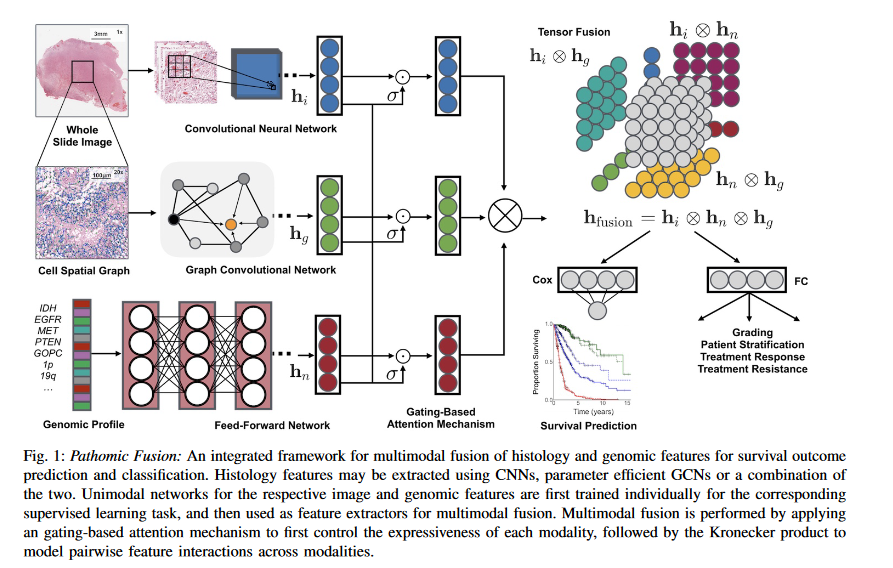
\includegraphics[width=0.8\textwidth]{images/image2.png}%
\caption{Image 3}%
\end{figure}

%


\begin{figure}[h!]%
\centering%
\includegraphics[width=0.8\textwidth]{images/image3.png}%
\caption{Image 4}%
\end{figure}

%


\begin{figure}[h!]%
\centering%
\includegraphics[width=0.8\textwidth]{images/image4.png}%
\caption{Image 5}%
\end{figure}

%


\begin{figure}[h!]%
\centering%
\includegraphics[width=0.8\textwidth]{images/image5.png}%
\caption{Image 6}%
\end{figure}

%


\begin{figure}[h!]%
\centering%
\includegraphics[width=0.8\textwidth]{images/image6.png}%
\caption{Image 7}%
\end{figure}

%


\begin{figure}[h!]%
\centering%
\includegraphics[width=0.8\textwidth]{images/image7.png}%
\caption{Image 8}%
\end{figure}

%


\begin{figure}[h!]%
\centering%
\includegraphics[width=0.8\textwidth]{images/image8.png}%
\caption{Image 9}%
\end{figure}

%


\begin{figure}[h!]%
\centering%
\includegraphics[width=0.8\textwidth]{images/image9.png}%
\caption{Image 10}%
\end{figure}

%


\begin{figure}[h!]%
\centering%
\includegraphics[width=0.8\textwidth]{images/image10.png}%
\caption{Image 11}%
\end{figure}

%


\begin{figure}[h!]%
\centering%
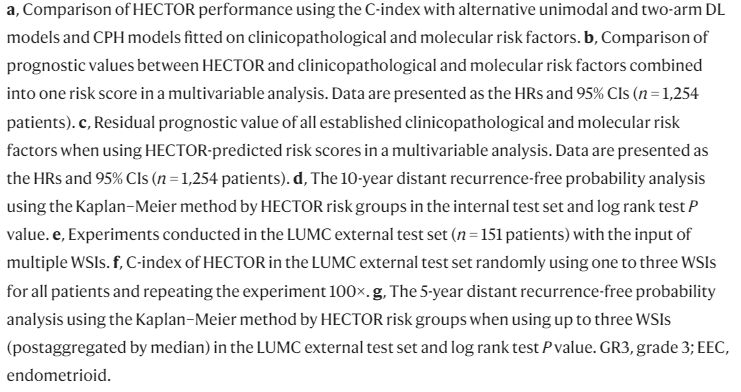
\includegraphics[width=0.8\textwidth]{images/image11.png}%
\caption{Image 12}%
\end{figure}

%


\begin{figure}[h!]%
\centering%
\includegraphics[width=0.8\textwidth]{images/image12.png}%
\caption{Image 13}%
\end{figure}

%


\begin{figure}[h!]%
\centering%
\includegraphics[width=0.8\textwidth]{images/image13.png}%
\caption{Image 14}%
\end{figure}

%


\begin{figure}[h!]%
\centering%
\includegraphics[width=0.8\textwidth]{images/image14.png}%
\caption{Image 15}%
\end{figure}

%


\begin{figure}[h!]%
\centering%
\includegraphics[width=0.8\textwidth]{images/image15.png}%
\caption{Image 16}%
\end{figure}

%


\begin{figure}[h!]%
\centering%
\includegraphics[width=0.8\textwidth]{images/image16.png}%
\caption{Image 17}%
\end{figure}

%


\begin{figure}[h!]%
\centering%
\includegraphics[width=0.8\textwidth]{images/image17.png}%
\caption{Image 18}%
\end{figure}

%


\begin{figure}[h!]%
\centering%
\includegraphics[width=0.8\textwidth]{images/image18.png}%
\caption{Image 19}%
\end{figure}

%


\begin{figure}[h!]%
\centering%
\includegraphics[width=0.8\textwidth]{images/image19.png}%
\caption{Image 20}%
\end{figure}

%


\begin{figure}[h!]%
\centering%
\includegraphics[width=0.8\textwidth]{images/image20.png}%
\caption{Image 21}%
\end{figure}

%


\begin{figure}[h!]%
\centering%
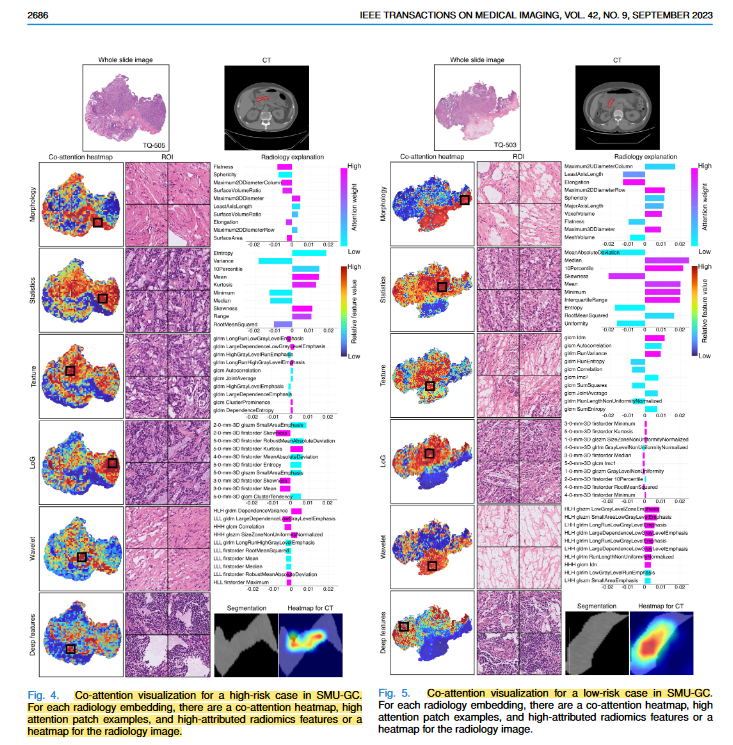
\includegraphics[width=0.8\textwidth]{images/image21.png}%
\caption{Image 22}%
\end{figure}

%


\begin{figure}[h!]%
\centering%
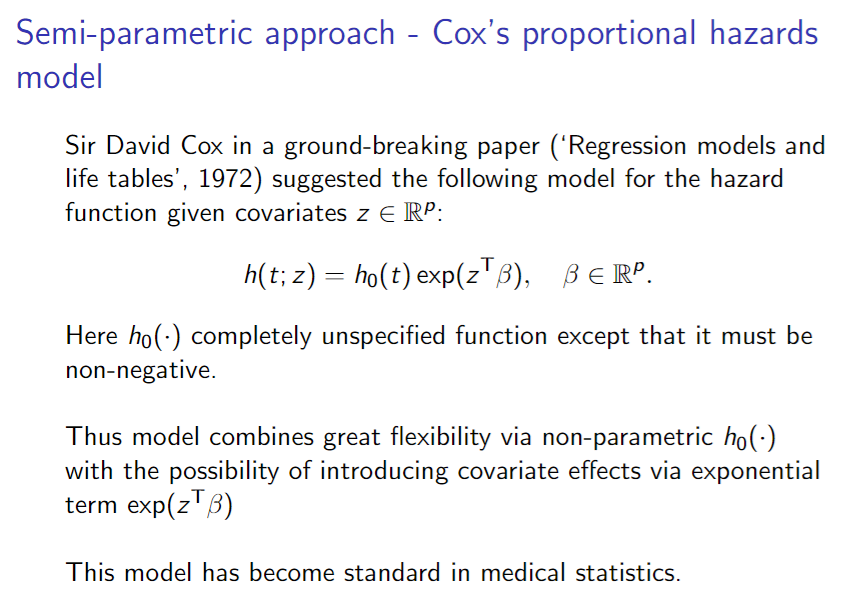
\includegraphics[width=0.8\textwidth]{images/image22.png}%
\caption{Image 23}%
\end{figure}

%


\begin{figure}[h!]%
\centering%
\includegraphics[width=0.8\textwidth]{images/image23.png}%
\caption{Image 24}%
\end{figure}

%


\begin{figure}[h!]%
\centering%
\includegraphics[width=0.8\textwidth]{images/image24.png}%
\caption{Image 25}%
\end{figure}

%


\begin{figure}[h!]%
\centering%
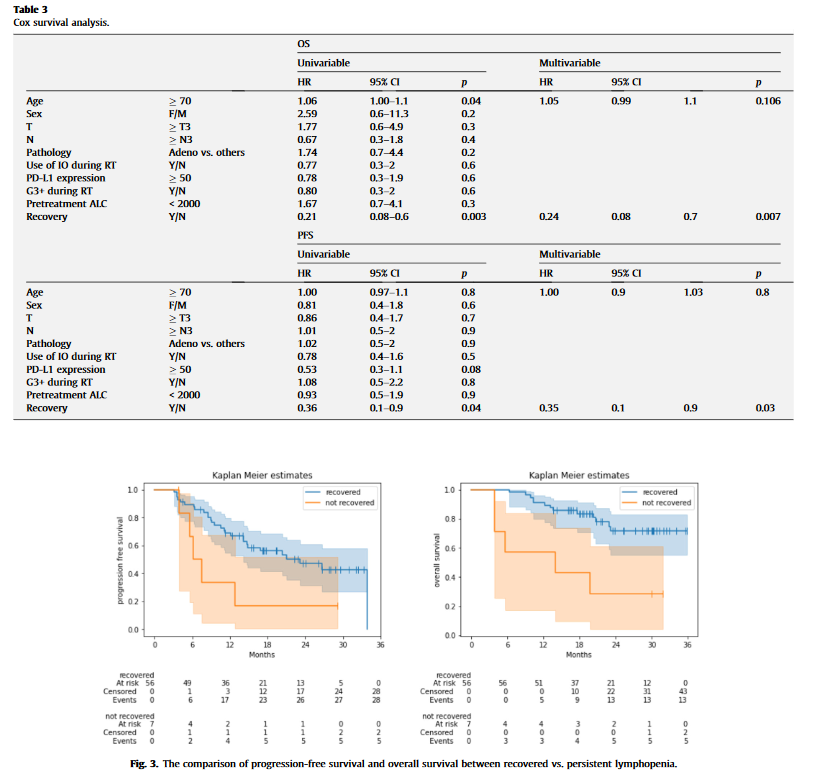
\includegraphics[width=0.8\textwidth]{images/image25.png}%
\caption{Image 26}%
\end{figure}

%


\begin{figure}[h!]%
\centering%
\includegraphics[width=0.8\textwidth]{images/image26.png}%
\caption{Image 27}%
\end{figure}

%


\begin{figure}[h!]%
\centering%
\includegraphics[width=0.8\textwidth]{images/image27.png}%
\caption{Image 28}%
\end{figure}

%


\begin{figure}[h!]%
\centering%
\includegraphics[width=0.8\textwidth]{images/image28.png}%
\caption{Image 29}%
\end{figure}

%


\begin{figure}[h!]%
\centering%
\includegraphics[width=0.8\textwidth]{images/image29.png}%
\caption{Image 30}%
\end{figure}

%


\begin{figure}[h!]%
\centering%
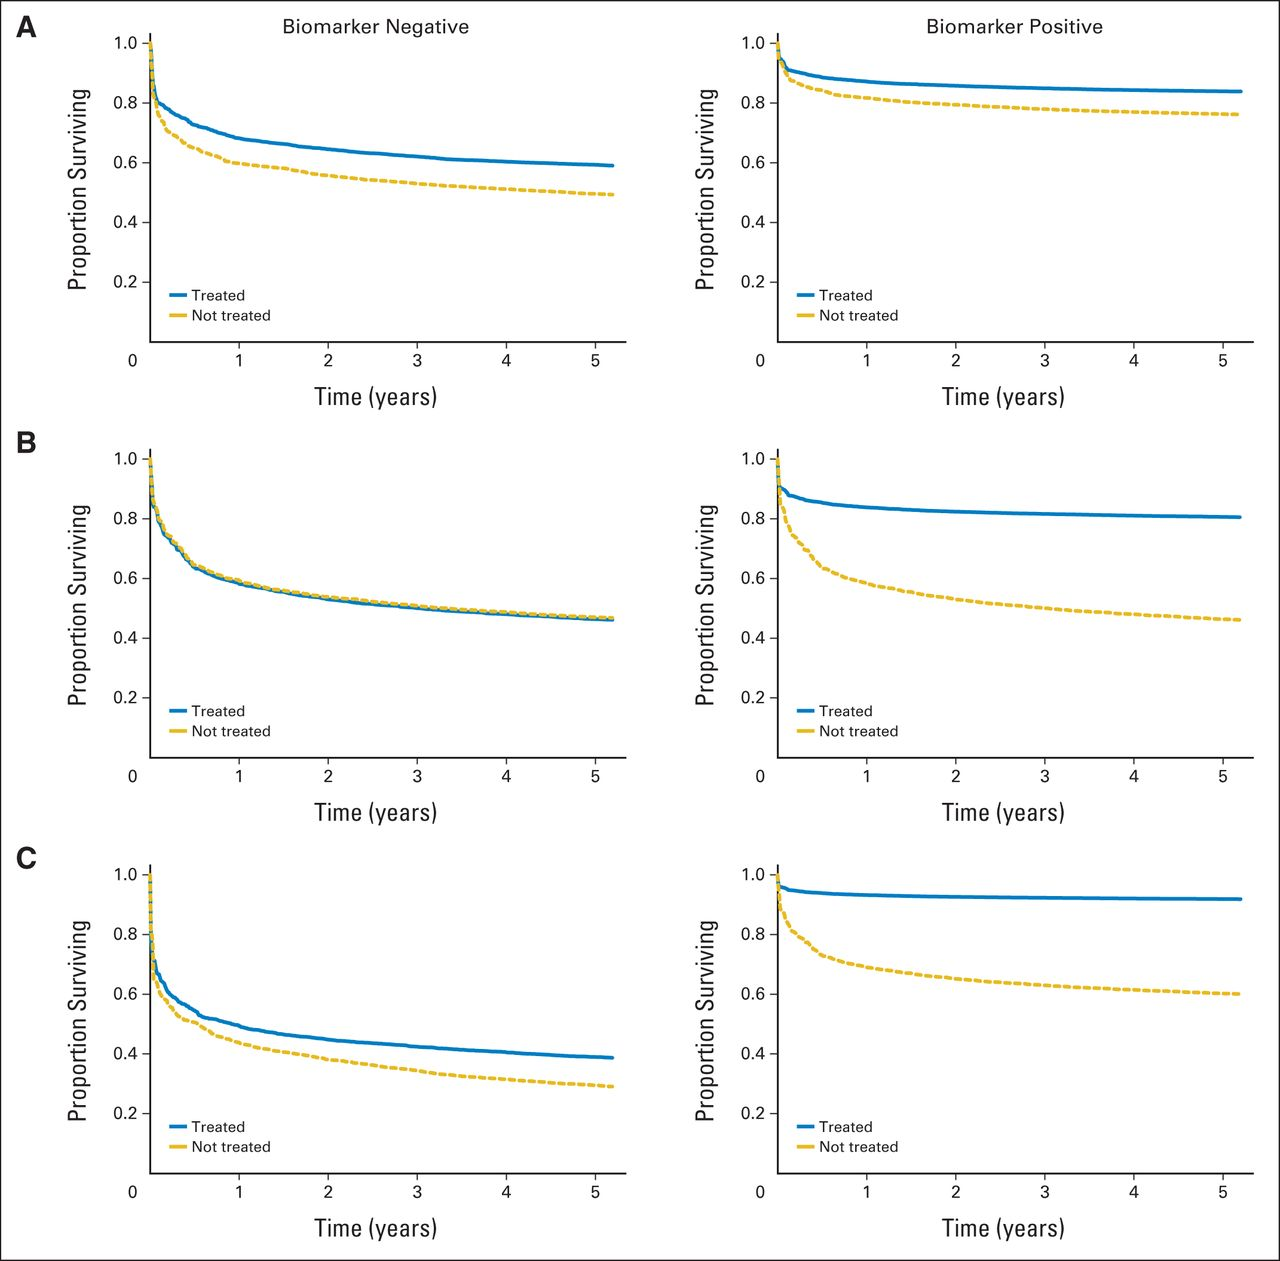
\includegraphics[width=0.8\textwidth]{images/image30.png}%
\caption{Image 31}%
\end{figure}

%


\begin{figure}[h!]%
\centering%
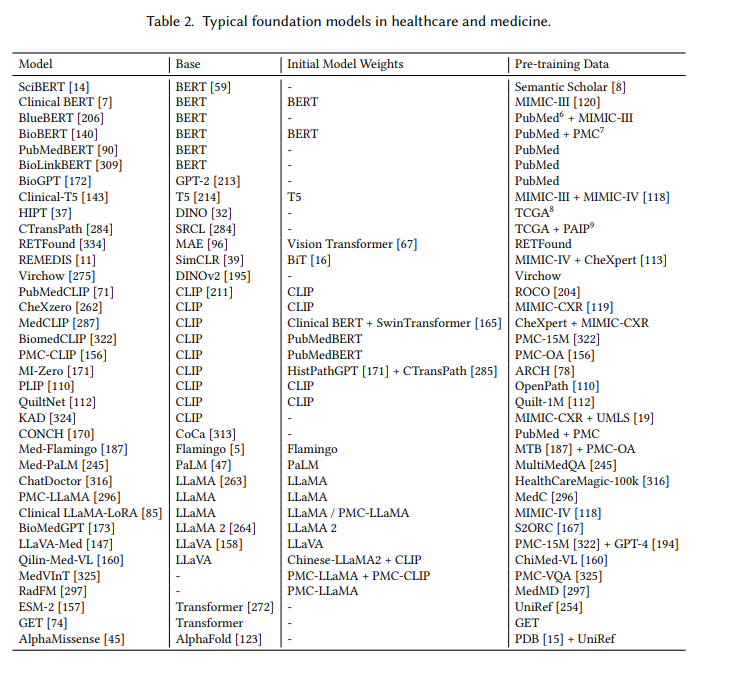
\includegraphics[width=0.8\textwidth]{images/image31.png}%
\caption{Image 32}%
\end{figure}

%


\begin{figure}[h!]%
\centering%
\includegraphics[width=0.8\textwidth]{images/image32.png}%
\caption{Image 33}%
\end{figure}

%


\begin{figure}[h!]%
\centering%
\includegraphics[width=0.8\textwidth]{images/image33.png}%
\caption{Image 34}%
\end{figure}

%


\begin{figure}[h!]%
\centering%
\includegraphics[width=0.8\textwidth]{images/image34.png}%
\caption{Image 35}%
\end{figure}

%


\begin{figure}[h!]%
\centering%
\includegraphics[width=0.8\textwidth]{images/image35.png}%
\caption{Image 36}%
\end{figure}

%


\begin{figure}[h!]%
\centering%
\includegraphics[width=0.8\textwidth]{images/image36.png}%
\caption{Image 37}%
\end{figure}

%


\begin{figure}[h!]%
\centering%
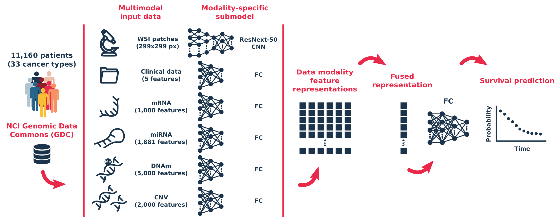
\includegraphics[width=0.8\textwidth]{images/image37.png}%
\caption{Image 38}%
\end{figure}

%


\begin{figure}[h!]%
\centering%
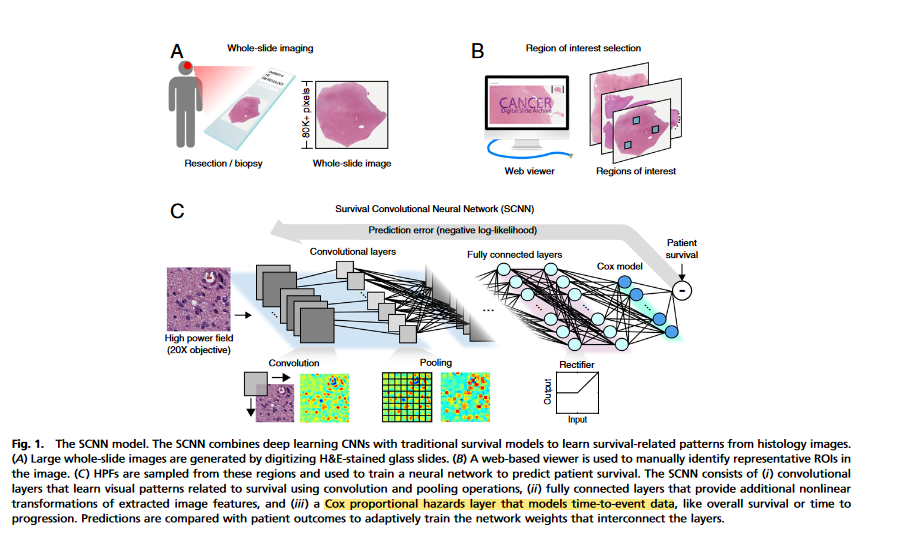
\includegraphics[width=0.8\textwidth]{images/image38.png}%
\caption{Image 39}%
\end{figure}

%


\begin{figure}[h!]%
\centering%
\includegraphics[width=0.8\textwidth]{images/image39.png}%
\caption{Image 40}%
\end{figure}

%


\begin{figure}[h!]%
\centering%
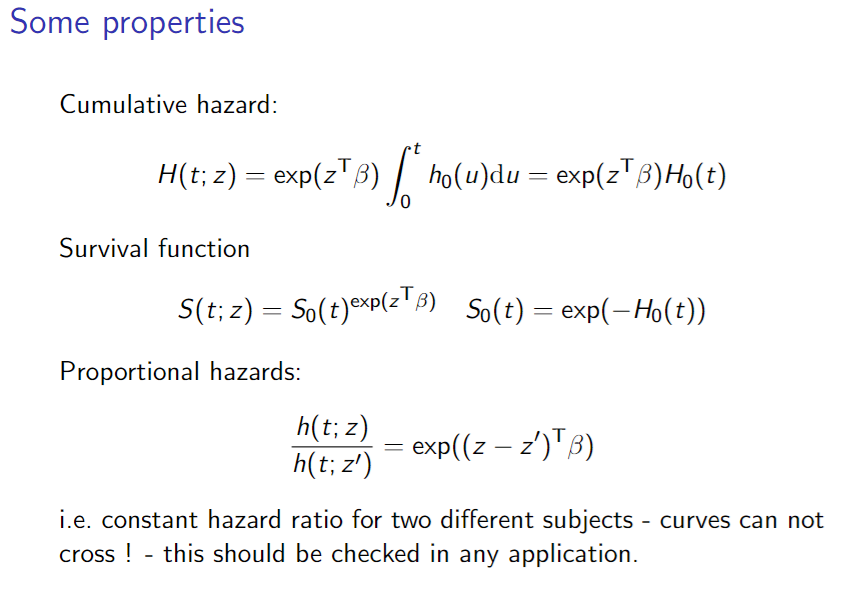
\includegraphics[width=0.8\textwidth]{images/image40.png}%
\caption{Image 41}%
\end{figure}

%


\begin{figure}[h!]%
\centering%
\includegraphics[width=0.8\textwidth]{images/image41.png}%
\caption{Image 42}%
\end{figure}

%


\begin{figure}[h!]%
\centering%
\includegraphics[width=0.8\textwidth]{images/image42.png}%
\caption{Image 43}%
\end{figure}

%


\begin{figure}[h!]%
\centering%
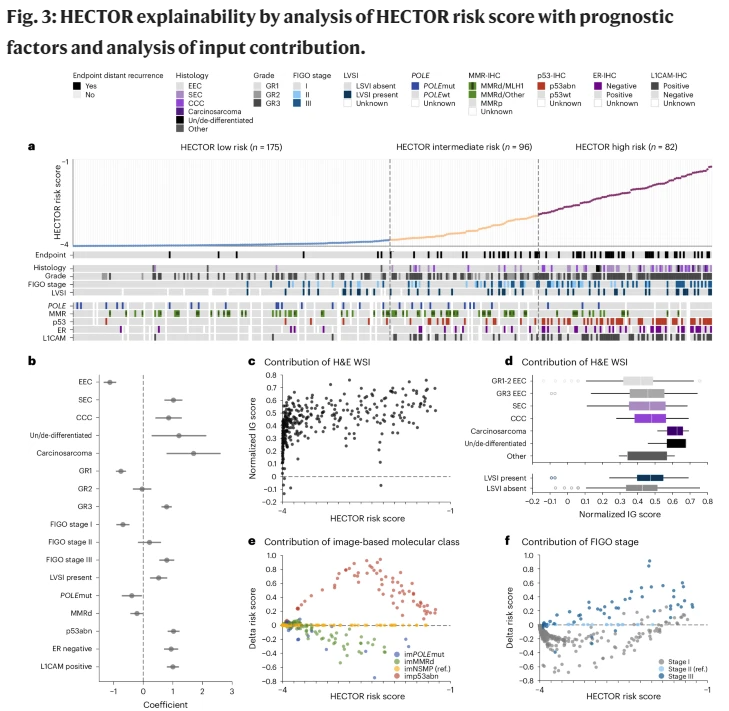
\includegraphics[width=0.8\textwidth]{images/image43.png}%
\caption{Image 44}%
\end{figure}

%


\begin{figure}[h!]%
\centering%
\includegraphics[width=0.8\textwidth]{images/image44.png}%
\caption{Image 45}%
\end{figure}

%


\begin{figure}[h!]%
\centering%
\includegraphics[width=0.8\textwidth]{images/image45.png}%
\caption{Image 46}%
\end{figure}

%


\begin{figure}[h!]%
\centering%
\includegraphics[width=0.8\textwidth]{images/image46.png}%
\caption{Image 47}%
\end{figure}

%


\begin{figure}[h!]%
\centering%
\includegraphics[width=0.8\textwidth]{images/image47.png}%
\caption{Image 48}%
\end{figure}

%


\begin{figure}[h!]%
\centering%
\includegraphics[width=0.8\textwidth]{images/image48.png}%
\caption{Image 49}%
\end{figure}

%


\begin{figure}[h!]%
\centering%
\includegraphics[width=0.8\textwidth]{images/image49.png}%
\caption{Image 50}%
\end{figure}

%


\begin{figure}[h!]%
\centering%
\includegraphics[width=0.8\textwidth]{images/image50.png}%
\caption{Image 51}%
\end{figure}

%


\begin{figure}[h!]%
\centering%
\includegraphics[width=0.8\textwidth]{images/image51.png}%
\caption{Image 52}%
\end{figure}

%


\begin{figure}[h!]%
\centering%
\includegraphics[width=0.8\textwidth]{images/image52.png}%
\caption{Image 53}%
\end{figure}

%


\begin{figure}[h!]%
\centering%
\includegraphics[width=0.8\textwidth]{images/image53.png}%
\caption{Image 54}%
\end{figure}

%


\begin{figure}[h!]%
\centering%
\includegraphics[width=0.8\textwidth]{images/image54.png}%
\caption{Image 55}%
\end{figure}

%


\begin{figure}[h!]%
\centering%
\includegraphics[width=0.8\textwidth]{images/image55.png}%
\caption{Image 56}%
\end{figure}

%


\begin{figure}[h!]%
\centering%
\includegraphics[width=0.8\textwidth]{images/image56.png}%
\caption{Image 57}%
\end{figure}

%


\begin{figure}[h!]%
\centering%
\includegraphics[width=0.8\textwidth]{images/image57.png}%
\caption{Image 58}%
\end{figure}

%


\begin{figure}[h!]%
\centering%
\includegraphics[width=0.8\textwidth]{images/image58.png}%
\caption{Image 59}%
\end{figure}

%


\begin{figure}[h!]%
\centering%
\includegraphics[width=0.8\textwidth]{images/image59.png}%
\caption{Image 60}%
\end{figure}

%


\begin{figure}[h!]%
\centering%
\includegraphics[width=0.8\textwidth]{images/image60.png}%
\caption{Image 61}%
\end{figure}

%


\begin{figure}[h!]%
\centering%
\includegraphics[width=0.8\textwidth]{images/image61.png}%
\caption{Image 62}%
\end{figure}

%


\begin{figure}[h!]%
\centering%
\includegraphics[width=0.8\textwidth]{images/image62.png}%
\caption{Image 63}%
\end{figure}

%


\begin{figure}[h!]%
\centering%
\includegraphics[width=0.8\textwidth]{images/image63.png}%
\caption{Image 64}%
\end{figure}

%


\begin{figure}[h!]%
\centering%
\includegraphics[width=0.8\textwidth]{images/image64.png}%
\caption{Image 65}%
\end{figure}

%


\begin{figure}[h!]%
\centering%
\includegraphics[width=0.8\textwidth]{images/image65.png}%
\caption{Image 66}%
\end{figure}

%


\begin{figure}[h!]%
\centering%
\includegraphics[width=0.8\textwidth]{images/image66.png}%
\caption{Image 67}%
\end{figure}

%


\begin{figure}[h!]%
\centering%
\includegraphics[width=0.8\textwidth]{images/image67.png}%
\caption{Image 68}%
\end{figure}

%


\begin{figure}[h!]%
\centering%
\includegraphics[width=0.8\textwidth]{images/image68.png}%
\caption{Image 69}%
\end{figure}

%


\begin{figure}[h!]%
\centering%
\includegraphics[width=0.8\textwidth]{images/image69.png}%
\caption{Image 70}%
\end{figure}

%


\begin{figure}[h!]%
\centering%
\includegraphics[width=0.8\textwidth]{images/image70.png}%
\caption{Image 71}%
\end{figure}

%


\begin{figure}[h!]%
\centering%
\includegraphics[width=0.8\textwidth]{images/image71.png}%
\caption{Image 72}%
\end{figure}

%


\begin{figure}[h!]%
\centering%
\includegraphics[width=0.8\textwidth]{images/image72.png}%
\caption{Image 73}%
\end{figure}

%


\begin{figure}[h!]%
\centering%
\includegraphics[width=0.8\textwidth]{images/image73.png}%
\caption{Image 74}%
\end{figure}

%


\begin{figure}[h!]%
\centering%
\includegraphics[width=0.8\textwidth]{images/image74.png}%
\caption{Image 75}%
\end{figure}

%


\begin{figure}[h!]%
\centering%
\includegraphics[width=0.8\textwidth]{images/image75.png}%
\caption{Image 76}%
\end{figure}

%


\begin{figure}[h!]%
\centering%
\includegraphics[width=0.8\textwidth]{images/image76.png}%
\caption{Image 77}%
\end{figure}

%


\begin{figure}[h!]%
\centering%
\includegraphics[width=0.8\textwidth]{images/image77.png}%
\caption{Image 78}%
\end{figure}

%


\begin{figure}[h!]%
\centering%
\includegraphics[width=0.8\textwidth]{images/image78.png}%
\caption{Image 79}%
\end{figure}

%


\begin{figure}[h!]%
\centering%
\includegraphics[width=0.8\textwidth]{images/image79.png}%
\caption{Image 80}%
\end{figure}

%


\begin{figure}[h!]%
\centering%
\includegraphics[width=0.8\textwidth]{images/image80.png}%
\caption{Image 81}%
\end{figure}

%


\begin{figure}[h!]%
\centering%
\includegraphics[width=0.8\textwidth]{images/image81.png}%
\caption{Image 82}%
\end{figure}

%


\begin{figure}[h!]%
\centering%
\includegraphics[width=0.8\textwidth]{images/image82.png}%
\caption{Image 83}%
\end{figure}

%


\begin{figure}[h!]%
\centering%
\includegraphics[width=0.8\textwidth]{images/image83.png}%
\caption{Image 84}%
\end{figure}

%


\begin{figure}[h!]%
\centering%
\includegraphics[width=0.8\textwidth]{images/image84.png}%
\caption{Image 85}%
\end{figure}

%


\begin{figure}[h!]%
\centering%
\includegraphics[width=0.8\textwidth]{images/image85.png}%
\caption{Image 86}%
\end{figure}

%


\begin{figure}[h!]%
\centering%
\includegraphics[width=0.8\textwidth]{images/image86.png}%
\caption{Image 87}%
\end{figure}

%


\begin{figure}[h!]%
\centering%
\includegraphics[width=0.8\textwidth]{images/image87.png}%
\caption{Image 88}%
\end{figure}

%


\begin{figure}[h!]%
\centering%
\includegraphics[width=0.8\textwidth]{images/image88.png}%
\caption{Image 89}%
\end{figure}

%


\begin{figure}[h!]%
\centering%
\includegraphics[width=0.8\textwidth]{images/image89.png}%
\caption{Image 90}%
\end{figure}

%


\begin{figure}[h!]%
\centering%
\includegraphics[width=0.8\textwidth]{images/image90.png}%
\caption{Image 91}%
\end{figure}

%


\begin{figure}[h!]%
\centering%
\includegraphics[width=0.8\textwidth]{images/image91.png}%
\caption{Image 92}%
\end{figure}

%


\begin{figure}[h!]%
\centering%
\includegraphics[width=0.8\textwidth]{images/image92.png}%
\caption{Image 93}%
\end{figure}

%


\begin{figure}[h!]%
\centering%
\includegraphics[width=0.8\textwidth]{images/image93.png}%
\caption{Image 94}%
\end{figure}

%


\begin{figure}[h!]%
\centering%
\includegraphics[width=0.8\textwidth]{images/image94.png}%
\caption{Image 95}%
\end{figure}

%


\begin{figure}[h!]%
\centering%
\includegraphics[width=0.8\textwidth]{images/image95.png}%
\caption{Image 96}%
\end{figure}

%


\begin{figure}[h!]%
\centering%
\includegraphics[width=0.8\textwidth]{images/image96.png}%
\caption{Image 97}%
\end{figure}

%


\begin{figure}[h!]%
\centering%
\includegraphics[width=0.8\textwidth]{images/image97.png}%
\caption{Image 98}%
\end{figure}

%


\begin{figure}[h!]%
\centering%
\includegraphics[width=0.8\textwidth]{images/image98.png}%
\caption{Image 99}%
\end{figure}

%


\begin{figure}[h!]%
\centering%
\includegraphics[width=0.8\textwidth]{images/image99.png}%
\caption{Image 100}%
\end{figure}

%


\begin{figure}[h!]%
\centering%
\includegraphics[width=0.8\textwidth]{images/image100.png}%
\caption{Image 101}%
\end{figure}

%


\begin{figure}[h!]%
\centering%
\includegraphics[width=0.8\textwidth]{images/image101.png}%
\caption{Image 102}%
\end{figure}

%


\begin{figure}[h!]%
\centering%
\includegraphics[width=0.8\textwidth]{images/image102.png}%
\caption{Image 103}%
\end{figure}

%


\begin{figure}[h!]%
\centering%
\includegraphics[width=0.8\textwidth]{images/image103.png}%
\caption{Image 104}%
\end{figure}

%


\begin{figure}[h!]%
\centering%
\includegraphics[width=0.8\textwidth]{images/image104.png}%
\caption{Image 105}%
\end{figure}

%


\begin{figure}[h!]%
\centering%
\includegraphics[width=0.8\textwidth]{images/image105.png}%
\caption{Image 106}%
\end{figure}

%


\begin{figure}[h!]%
\centering%
\includegraphics[width=0.8\textwidth]{images/image106.png}%
\caption{Image 107}%
\end{figure}

%


\begin{figure}[h!]%
\centering%
\includegraphics[width=0.8\textwidth]{images/image107.png}%
\caption{Image 108}%
\end{figure}

%


\begin{figure}[h!]%
\centering%
\includegraphics[width=0.8\textwidth]{images/image108.png}%
\caption{Image 109}%
\end{figure}

%


\begin{figure}[h!]%
\centering%
\includegraphics[width=0.8\textwidth]{images/image109.png}%
\caption{Image 110}%
\end{figure}

%


\begin{figure}[h!]%
\centering%
\includegraphics[width=0.8\textwidth]{images/image110.png}%
\caption{Image 111}%
\end{figure}

%


\begin{figure}[h!]%
\centering%
\includegraphics[width=0.8\textwidth]{images/image111.png}%
\caption{Image 112}%
\end{figure}

%


\begin{figure}[h!]%
\centering%
\includegraphics[width=0.8\textwidth]{images/image112.png}%
\caption{Image 113}%
\end{figure}

%


\begin{figure}[h!]%
\centering%
\includegraphics[width=0.8\textwidth]{images/image113.png}%
\caption{Image 114}%
\end{figure}

%


\begin{figure}[h!]%
\centering%
\includegraphics[width=0.8\textwidth]{images/image114.png}%
\caption{Image 115}%
\end{figure}

%


\begin{figure}[h!]%
\centering%
\includegraphics[width=0.8\textwidth]{images/image115.png}%
\caption{Image 116}%
\end{figure}

%


\begin{figure}[h!]%
\centering%
\includegraphics[width=0.8\textwidth]{images/image116.png}%
\caption{Image 117}%
\end{figure}

%


\begin{figure}[h!]%
\centering%
\includegraphics[width=0.8\textwidth]{images/image117.png}%
\caption{Image 118}%
\end{figure}

%


\begin{figure}[h!]%
\centering%
\includegraphics[width=0.8\textwidth]{images/image118.png}%
\caption{Image 119}%
\end{figure}

%


\begin{figure}[h!]%
\centering%
\includegraphics[width=0.8\textwidth]{images/image119.png}%
\caption{Image 120}%
\end{figure}

%


\begin{figure}[h!]%
\centering%
\includegraphics[width=0.8\textwidth]{images/image120.png}%
\caption{Image 121}%
\end{figure}

%


\begin{figure}[h!]%
\centering%
\includegraphics[width=0.8\textwidth]{images/image121.png}%
\caption{Image 122}%
\end{figure}

%


\begin{figure}[h!]%
\centering%
\includegraphics[width=0.8\textwidth]{images/image122.png}%
\caption{Image 123}%
\end{figure}

%


\begin{figure}[h!]%
\centering%
\includegraphics[width=0.8\textwidth]{images/image123.png}%
\caption{Image 124}%
\end{figure}

%


\begin{figure}[h!]%
\centering%
\includegraphics[width=0.8\textwidth]{images/image124.png}%
\caption{Image 125}%
\end{figure}

%


\begin{figure}[h!]%
\centering%
\includegraphics[width=0.8\textwidth]{images/image125.png}%
\caption{Image 126}%
\end{figure}

%


\begin{figure}[h!]%
\centering%
\includegraphics[width=0.8\textwidth]{images/image126.png}%
\caption{Image 127}%
\end{figure}

%


\begin{figure}[h!]%
\centering%
\includegraphics[width=0.8\textwidth]{images/image127.png}%
\caption{Image 128}%
\end{figure}

%


\begin{figure}[h!]%
\centering%
\includegraphics[width=0.8\textwidth]{images/image128.png}%
\caption{Image 129}%
\end{figure}

%


\begin{figure}[h!]%
\centering%
\includegraphics[width=0.8\textwidth]{images/image129.png}%
\caption{Image 130}%
\end{figure}

%


\begin{figure}[h!]%
\centering%
\includegraphics[width=0.8\textwidth]{images/image130.png}%
\caption{Image 131}%
\end{figure}

%


\begin{figure}[h!]%
\centering%
\includegraphics[width=0.8\textwidth]{images/image131.png}%
\caption{Image 132}%
\end{figure}

%


\begin{figure}[h!]%
\centering%
\includegraphics[width=0.8\textwidth]{images/image132.png}%
\caption{Image 133}%
\end{figure}

%


\begin{figure}[h!]%
\centering%
\includegraphics[width=0.8\textwidth]{images/image133.png}%
\caption{Image 134}%
\end{figure}

%


\begin{figure}[h!]%
\centering%
\includegraphics[width=0.8\textwidth]{images/image134.png}%
\caption{Image 135}%
\end{figure}

%


\begin{figure}[h!]%
\centering%
\includegraphics[width=0.8\textwidth]{images/image135.png}%
\caption{Image 136}%
\end{figure}

%


\begin{figure}[h!]%
\centering%
\includegraphics[width=0.8\textwidth]{images/image136.png}%
\caption{Image 137}%
\end{figure}

%


\begin{figure}[h!]%
\centering%
\includegraphics[width=0.8\textwidth]{images/image137.png}%
\caption{Image 138}%
\end{figure}

%


\begin{figure}[h!]%
\centering%
\includegraphics[width=0.8\textwidth]{images/image138.png}%
\caption{Image 139}%
\end{figure}

%


\begin{figure}[h!]%
\centering%
\includegraphics[width=0.8\textwidth]{images/image139.png}%
\caption{Image 140}%
\end{figure}

%


\begin{figure}[h!]%
\centering%
\includegraphics[width=0.8\textwidth]{images/image140.png}%
\caption{Image 141}%
\end{figure}

%


\begin{figure}[h!]%
\centering%
\includegraphics[width=0.8\textwidth]{images/image141.png}%
\caption{Image 142}%
\end{figure}

%


\begin{figure}[h!]%
\centering%
\includegraphics[width=0.8\textwidth]{images/image142.png}%
\caption{Image 143}%
\end{figure}

%


\begin{figure}[h!]%
\centering%
\includegraphics[width=0.8\textwidth]{images/image143.png}%
\caption{Image 144}%
\end{figure}

%


\begin{figure}[h!]%
\centering%
\includegraphics[width=0.8\textwidth]{images/image144.png}%
\caption{Image 145}%
\end{figure}

%


\begin{figure}[h!]%
\centering%
\includegraphics[width=0.8\textwidth]{images/image145.png}%
\caption{Image 146}%
\end{figure}

%


\begin{figure}[h!]%
\centering%
\includegraphics[width=0.8\textwidth]{images/image146.png}%
\caption{Image 147}%
\end{figure}

%


\begin{figure}[h!]%
\centering%
\includegraphics[width=0.8\textwidth]{images/image147.png}%
\caption{Image 148}%
\end{figure}

%


\begin{figure}[h!]%
\centering%
\includegraphics[width=0.8\textwidth]{images/image148.png}%
\caption{Image 149}%
\end{figure}

%


\begin{figure}[h!]%
\centering%
\includegraphics[width=0.8\textwidth]{images/image149.png}%
\caption{Image 150}%
\end{figure}

%


\begin{figure}[h!]%
\centering%
\includegraphics[width=0.8\textwidth]{images/image150.png}%
\caption{Image 151}%
\end{figure}

%


\begin{figure}[h!]%
\centering%
\includegraphics[width=0.8\textwidth]{images/image151.png}%
\caption{Image 152}%
\end{figure}

%


\begin{figure}[h!]%
\centering%
\includegraphics[width=0.8\textwidth]{images/image152.png}%
\caption{Image 153}%
\end{figure}

%


\begin{figure}[h!]%
\centering%
\includegraphics[width=0.8\textwidth]{images/image153.png}%
\caption{Image 154}%
\end{figure}

%


\begin{figure}[h!]%
\centering%
\includegraphics[width=0.8\textwidth]{images/image154.png}%
\caption{Image 155}%
\end{figure}

%


\begin{figure}[h!]%
\centering%
\includegraphics[width=0.8\textwidth]{images/image155.png}%
\caption{Image 156}%
\end{figure}

%


\begin{figure}[h!]%
\centering%
\includegraphics[width=0.8\textwidth]{images/image156.png}%
\caption{Image 157}%
\end{figure}

%


\begin{figure}[h!]%
\centering%
\includegraphics[width=0.8\textwidth]{images/image157.png}%
\caption{Image 158}%
\end{figure}

%


\begin{figure}[h!]%
\centering%
\includegraphics[width=0.8\textwidth]{images/image158.png}%
\caption{Image 159}%
\end{figure}

%


\begin{figure}[h!]%
\centering%
\includegraphics[width=0.8\textwidth]{images/image159.png}%
\caption{Image 160}%
\end{figure}

%


\begin{figure}[h!]%
\centering%
\includegraphics[width=0.8\textwidth]{images/image160.png}%
\caption{Image 161}%
\end{figure}

%


\begin{figure}[h!]%
\centering%
\includegraphics[width=0.8\textwidth]{images/image161.png}%
\caption{Image 162}%
\end{figure}

%


\begin{figure}[h!]%
\centering%
\includegraphics[width=0.8\textwidth]{images/image162.png}%
\caption{Image 163}%
\end{figure}

%


\begin{figure}[h!]%
\centering%
\includegraphics[width=0.8\textwidth]{images/image163.png}%
\caption{Image 164}%
\end{figure}

%


\begin{figure}[h!]%
\centering%
\includegraphics[width=0.8\textwidth]{images/image164.png}%
\caption{Image 165}%
\end{figure}

%


\begin{figure}[h!]%
\centering%
\includegraphics[width=0.8\textwidth]{images/image165.png}%
\caption{Image 166}%
\end{figure}

%


\begin{figure}[h!]%
\centering%
\includegraphics[width=0.8\textwidth]{images/image166.png}%
\caption{Image 167}%
\end{figure}

%


\begin{figure}[h!]%
\centering%
\includegraphics[width=0.8\textwidth]{images/image167.png}%
\caption{Image 168}%
\end{figure}

%


\begin{figure}[h!]%
\centering%
\includegraphics[width=0.8\textwidth]{images/image168.png}%
\caption{Image 169}%
\end{figure}

%


\begin{figure}[h!]%
\centering%
\includegraphics[width=0.8\textwidth]{images/image169.png}%
\caption{Image 170}%
\end{figure}

%


\begin{figure}[h!]%
\centering%
\includegraphics[width=0.8\textwidth]{images/image170.png}%
\caption{Image 171}%
\end{figure}

%


\begin{figure}[h!]%
\centering%
\includegraphics[width=0.8\textwidth]{images/image171.png}%
\caption{Image 172}%
\end{figure}

%


\begin{figure}[h!]%
\centering%
\includegraphics[width=0.8\textwidth]{images/image172.png}%
\caption{Image 173}%
\end{figure}

%


\begin{figure}[h!]%
\centering%
\includegraphics[width=0.8\textwidth]{images/image173.png}%
\caption{Image 174}%
\end{figure}

%


\begin{figure}[h!]%
\centering%
\includegraphics[width=0.8\textwidth]{images/image174.png}%
\caption{Image 175}%
\end{figure}

%


\begin{figure}[h!]%
\centering%
\includegraphics[width=0.8\textwidth]{images/image175.png}%
\caption{Image 176}%
\end{figure}

%


\begin{figure}[h!]%
\centering%
\includegraphics[width=0.8\textwidth]{images/image176.png}%
\caption{Image 177}%
\end{figure}

%


\begin{figure}[h!]%
\centering%
\includegraphics[width=0.8\textwidth]{images/image177.png}%
\caption{Image 178}%
\end{figure}

%


\begin{figure}[h!]%
\centering%
\includegraphics[width=0.8\textwidth]{images/image178.png}%
\caption{Image 179}%
\end{figure}

%


\begin{figure}[h!]%
\centering%
\includegraphics[width=0.8\textwidth]{images/image179.png}%
\caption{Image 180}%
\end{figure}

%


\begin{figure}[h!]%
\centering%
\includegraphics[width=0.8\textwidth]{images/image180.png}%
\caption{Image 181}%
\end{figure}

%


\begin{figure}[h!]%
\centering%
\includegraphics[width=0.8\textwidth]{images/image181.png}%
\caption{Image 182}%
\end{figure}

%


\begin{figure}[h!]%
\centering%
\includegraphics[width=0.8\textwidth]{images/image182.png}%
\caption{Image 183}%
\end{figure}

%


\begin{figure}[h!]%
\centering%
\includegraphics[width=0.8\textwidth]{images/image183.png}%
\caption{Image 184}%
\end{figure}

%


\begin{figure}[h!]%
\centering%
\includegraphics[width=0.8\textwidth]{images/image184.png}%
\caption{Image 185}%
\end{figure}

%


\begin{figure}[h!]%
\centering%
\includegraphics[width=0.8\textwidth]{images/image185.png}%
\caption{Image 186}%
\end{figure}

%


\begin{figure}[h!]%
\centering%
\includegraphics[width=0.8\textwidth]{images/image186.png}%
\caption{Image 187}%
\end{figure}

%


\begin{figure}[h!]%
\centering%
\includegraphics[width=0.8\textwidth]{images/image187.png}%
\caption{Image 188}%
\end{figure}

%


\begin{figure}[h!]%
\centering%
\includegraphics[width=0.8\textwidth]{images/image188.png}%
\caption{Image 189}%
\end{figure}

%


\begin{figure}[h!]%
\centering%
\includegraphics[width=0.8\textwidth]{images/image189.png}%
\caption{Image 190}%
\end{figure}

%


\begin{figure}[h!]%
\centering%
\includegraphics[width=0.8\textwidth]{images/image190.png}%
\caption{Image 191}%
\end{figure}

%


\begin{figure}[h!]%
\centering%
\includegraphics[width=0.8\textwidth]{images/image191.png}%
\caption{Image 192}%
\end{figure}

%


\begin{figure}[h!]%
\centering%
\includegraphics[width=0.8\textwidth]{images/image192.png}%
\caption{Image 193}%
\end{figure}

%


\begin{figure}[h!]%
\centering%
\includegraphics[width=0.8\textwidth]{images/image193.png}%
\caption{Image 194}%
\end{figure}

%


\begin{figure}[h!]%
\centering%
\includegraphics[width=0.8\textwidth]{images/image194.png}%
\caption{Image 195}%
\end{figure}

%


\begin{figure}[h!]%
\centering%
\includegraphics[width=0.8\textwidth]{images/image195.png}%
\caption{Image 196}%
\end{figure}

%


\begin{figure}[h!]%
\centering%
\includegraphics[width=0.8\textwidth]{images/image196.png}%
\caption{Image 197}%
\end{figure}

%


\begin{figure}[h!]%
\centering%
\includegraphics[width=0.8\textwidth]{images/image197.png}%
\caption{Image 198}%
\end{figure}

%


\begin{figure}[h!]%
\centering%
\includegraphics[width=0.8\textwidth]{images/image198.png}%
\caption{Image 199}%
\end{figure}

%


\begin{figure}[h!]%
\centering%
\includegraphics[width=0.8\textwidth]{images/image199.png}%
\caption{Image 200}%
\end{figure}

%


\begin{figure}[h!]%
\centering%
\includegraphics[width=0.8\textwidth]{images/image200.png}%
\caption{Image 201}%
\end{figure}

%


\begin{figure}[h!]%
\centering%
\includegraphics[width=0.8\textwidth]{images/image201.png}%
\caption{Image 202}%
\end{figure}

%


\begin{figure}[h!]%
\centering%
\includegraphics[width=0.8\textwidth]{images/image202.png}%
\caption{Image 203}%
\end{figure}

%


\begin{figure}[h!]%
\centering%
\includegraphics[width=0.8\textwidth]{images/image203.png}%
\caption{Image 204}%
\end{figure}

%


\begin{figure}[h!]%
\centering%
\includegraphics[width=0.8\textwidth]{images/image204.png}%
\caption{Image 205}%
\end{figure}

%


\begin{figure}[h!]%
\centering%
\includegraphics[width=0.8\textwidth]{images/image205.png}%
\caption{Image 206}%
\end{figure}

%


\begin{figure}[h!]%
\centering%
\includegraphics[width=0.8\textwidth]{images/image206.png}%
\caption{Image 207}%
\end{figure}

%


\begin{figure}[h!]%
\centering%
\includegraphics[width=0.8\textwidth]{images/image207.png}%
\caption{Image 208}%
\end{figure}

%


\begin{figure}[h!]%
\centering%
\includegraphics[width=0.8\textwidth]{images/image208.png}%
\caption{Image 209}%
\end{figure}

%


\begin{figure}[h!]%
\centering%
\includegraphics[width=0.8\textwidth]{images/image209.png}%
\caption{Image 210}%
\end{figure}

%


\begin{figure}[h!]%
\centering%
\includegraphics[width=0.8\textwidth]{images/image210.png}%
\caption{Image 211}%
\end{figure}

%


\begin{figure}[h!]%
\centering%
\includegraphics[width=0.8\textwidth]{images/image211.png}%
\caption{Image 212}%
\end{figure}

%


\begin{figure}[h!]%
\centering%
\includegraphics[width=0.8\textwidth]{images/image212.png}%
\caption{Image 213}%
\end{figure}

%


\begin{figure}[h!]%
\centering%
\includegraphics[width=0.8\textwidth]{images/image213.png}%
\caption{Image 214}%
\end{figure}

%


\begin{figure}[h!]%
\centering%
\includegraphics[width=0.8\textwidth]{images/image214.png}%
\caption{Image 215}%
\end{figure}

%


\begin{figure}[h!]%
\centering%
\includegraphics[width=0.8\textwidth]{images/image215.png}%
\caption{Image 216}%
\end{figure}

%


\begin{figure}[h!]%
\centering%
\includegraphics[width=0.8\textwidth]{images/image216.png}%
\caption{Image 217}%
\end{figure}

%


\begin{figure}[h!]%
\centering%
\includegraphics[width=0.8\textwidth]{images/image217.png}%
\caption{Image 218}%
\end{figure}

%


\begin{figure}[h!]%
\centering%
\includegraphics[width=0.8\textwidth]{images/image218.png}%
\caption{Image 219}%
\end{figure}

%


\begin{figure}[h!]%
\centering%
\includegraphics[width=0.8\textwidth]{images/image219.png}%
\caption{Image 220}%
\end{figure}

%


\begin{figure}[h!]%
\centering%
\includegraphics[width=0.8\textwidth]{images/image220.png}%
\caption{Image 221}%
\end{figure}

%


\begin{figure}[h!]%
\centering%
\includegraphics[width=0.8\textwidth]{images/image221.png}%
\caption{Image 222}%
\end{figure}

%


\begin{figure}[h!]%
\centering%
\includegraphics[width=0.8\textwidth]{images/image222.png}%
\caption{Image 223}%
\end{figure}

%


\begin{figure}[h!]%
\centering%
\includegraphics[width=0.8\textwidth]{images/image223.png}%
\caption{Image 224}%
\end{figure}

%


\begin{figure}[h!]%
\centering%
\includegraphics[width=0.8\textwidth]{images/image224.png}%
\caption{Image 225}%
\end{figure}

%


\begin{figure}[h!]%
\centering%
\includegraphics[width=0.8\textwidth]{images/image225.png}%
\caption{Image 226}%
\end{figure}

%


\begin{figure}[h!]%
\centering%
\includegraphics[width=0.8\textwidth]{images/image226.png}%
\caption{Image 227}%
\end{figure}

%


\begin{figure}[h!]%
\centering%
\includegraphics[width=0.8\textwidth]{images/image227.png}%
\caption{Image 228}%
\end{figure}

%


\begin{figure}[h!]%
\centering%
\includegraphics[width=0.8\textwidth]{images/image228.png}%
\caption{Image 229}%
\end{figure}

%


\begin{figure}[h!]%
\centering%
\includegraphics[width=0.8\textwidth]{images/image229.png}%
\caption{Image 230}%
\end{figure}

%


\begin{figure}[h!]%
\centering%
\includegraphics[width=0.8\textwidth]{images/image230.png}%
\caption{Image 231}%
\end{figure}

%


\begin{figure}[h!]%
\centering%
\includegraphics[width=0.8\textwidth]{images/image231.png}%
\caption{Image 232}%
\end{figure}

%


\begin{figure}[h!]%
\centering%
\includegraphics[width=0.8\textwidth]{images/image232.png}%
\caption{Image 233}%
\end{figure}

%


\begin{figure}[h!]%
\centering%
\includegraphics[width=0.8\textwidth]{images/image233.png}%
\caption{Image 234}%
\end{figure}

%


\begin{figure}[h!]%
\centering%
\includegraphics[width=0.8\textwidth]{images/image234.png}%
\caption{Image 235}%
\end{figure}

%


\begin{figure}[h!]%
\centering%
\includegraphics[width=0.8\textwidth]{images/image235.png}%
\caption{Image 236}%
\end{figure}

%


\begin{figure}[h!]%
\centering%
\includegraphics[width=0.8\textwidth]{images/image236.png}%
\caption{Image 237}%
\end{figure}

%


\begin{figure}[h!]%
\centering%
\includegraphics[width=0.8\textwidth]{images/image237.png}%
\caption{Image 238}%
\end{figure}

%


\begin{figure}[h!]%
\centering%
\includegraphics[width=0.8\textwidth]{images/image238.png}%
\caption{Image 239}%
\end{figure}

%


\begin{figure}[h!]%
\centering%
\includegraphics[width=0.8\textwidth]{images/image239.png}%
\caption{Image 240}%
\end{figure}

%


\begin{figure}[h!]%
\centering%
\includegraphics[width=0.8\textwidth]{images/image240.png}%
\caption{Image 241}%
\end{figure}

%


\begin{figure}[h!]%
\centering%
\includegraphics[width=0.8\textwidth]{images/image241.png}%
\caption{Image 242}%
\end{figure}

%


\begin{figure}[h!]%
\centering%
\includegraphics[width=0.8\textwidth]{images/image242.png}%
\caption{Image 243}%
\end{figure}

%


\begin{figure}[h!]%
\centering%
\includegraphics[width=0.8\textwidth]{images/image243.png}%
\caption{Image 244}%
\end{figure}

%


\begin{figure}[h!]%
\centering%
\includegraphics[width=0.8\textwidth]{images/image244.png}%
\caption{Image 245}%
\end{figure}

%


\begin{figure}[h!]%
\centering%
\includegraphics[width=0.8\textwidth]{images/image245.png}%
\caption{Image 246}%
\end{figure}

%


\begin{figure}[h!]%
\centering%
\includegraphics[width=0.8\textwidth]{images/image246.png}%
\caption{Image 247}%
\end{figure}

%


\begin{figure}[h!]%
\centering%
\includegraphics[width=0.8\textwidth]{images/image247.png}%
\caption{Image 248}%
\end{figure}

%


\begin{figure}[h!]%
\centering%
\includegraphics[width=0.8\textwidth]{images/image248.png}%
\caption{Image 249}%
\end{figure}

%


\begin{figure}[h!]%
\centering%
\includegraphics[width=0.8\textwidth]{images/image249.png}%
\caption{Image 250}%
\end{figure}

%


\begin{figure}[h!]%
\centering%
\includegraphics[width=0.8\textwidth]{images/image250.png}%
\caption{Image 251}%
\end{figure}

%


\begin{figure}[h!]%
\centering%
\includegraphics[width=0.8\textwidth]{images/image251.png}%
\caption{Image 252}%
\end{figure}

%


\begin{figure}[h!]%
\centering%
\includegraphics[width=0.8\textwidth]{images/image252.png}%
\caption{Image 253}%
\end{figure}

%


\begin{figure}[h!]%
\centering%
\includegraphics[width=0.8\textwidth]{images/image253.png}%
\caption{Image 254}%
\end{figure}

%


\begin{figure}[h!]%
\centering%
\includegraphics[width=0.8\textwidth]{images/image254.png}%
\caption{Image 255}%
\end{figure}

%


\begin{figure}[h!]%
\centering%
\includegraphics[width=0.8\textwidth]{images/image255.png}%
\caption{Image 256}%
\end{figure}

%


\begin{figure}[h!]%
\centering%
\includegraphics[width=0.8\textwidth]{images/image256.png}%
\caption{Image 257}%
\end{figure}

%


\begin{figure}[h!]%
\centering%
\includegraphics[width=0.8\textwidth]{images/image257.png}%
\caption{Image 258}%
\end{figure}

%


\begin{figure}[h!]%
\centering%
\includegraphics[width=0.8\textwidth]{images/image258.png}%
\caption{Image 259}%
\end{figure}

%


\begin{figure}[h!]%
\centering%
\includegraphics[width=0.8\textwidth]{images/image259.png}%
\caption{Image 260}%
\end{figure}

%


\begin{figure}[h!]%
\centering%
\includegraphics[width=0.8\textwidth]{images/image260.png}%
\caption{Image 261}%
\end{figure}

%


\begin{figure}[h!]%
\centering%
\includegraphics[width=0.8\textwidth]{images/image261.png}%
\caption{Image 262}%
\end{figure}

%


\begin{figure}[h!]%
\centering%
\includegraphics[width=0.8\textwidth]{images/image262.png}%
\caption{Image 263}%
\end{figure}

%


\begin{figure}[h!]%
\centering%
\includegraphics[width=0.8\textwidth]{images/image263.png}%
\caption{Image 264}%
\end{figure}

%


\begin{figure}[h!]%
\centering%
\includegraphics[width=0.8\textwidth]{images/image264.png}%
\caption{Image 265}%
\end{figure}

%


\begin{figure}[h!]%
\centering%
\includegraphics[width=0.8\textwidth]{images/image265.png}%
\caption{Image 266}%
\end{figure}

%


\begin{figure}[h!]%
\centering%
\includegraphics[width=0.8\textwidth]{images/image266.png}%
\caption{Image 267}%
\end{figure}

%


\begin{figure}[h!]%
\centering%
\includegraphics[width=0.8\textwidth]{images/image267.png}%
\caption{Image 268}%
\end{figure}

%


\begin{figure}[h!]%
\centering%
\includegraphics[width=0.8\textwidth]{images/image268.png}%
\caption{Image 269}%
\end{figure}

%


\begin{figure}[h!]%
\centering%
\includegraphics[width=0.8\textwidth]{images/image269.png}%
\caption{Image 270}%
\end{figure}

%


\begin{figure}[h!]%
\centering%
\includegraphics[width=0.8\textwidth]{images/image270.png}%
\caption{Image 271}%
\end{figure}

%


\begin{figure}[h!]%
\centering%
\includegraphics[width=0.8\textwidth]{images/image271.png}%
\caption{Image 272}%
\end{figure}

%


\begin{figure}[h!]%
\centering%
\includegraphics[width=0.8\textwidth]{images/image272.png}%
\caption{Image 273}%
\end{figure}

%


\begin{figure}[h!]%
\centering%
\includegraphics[width=0.8\textwidth]{images/image273.png}%
\caption{Image 274}%
\end{figure}

%


\begin{figure}[h!]%
\centering%
\includegraphics[width=0.8\textwidth]{images/image274.png}%
\caption{Image 275}%
\end{figure}

%


\begin{figure}[h!]%
\centering%
\includegraphics[width=0.8\textwidth]{images/image275.png}%
\caption{Image 276}%
\end{figure}

%


\begin{figure}[h!]%
\centering%
\includegraphics[width=0.8\textwidth]{images/image276.png}%
\caption{Image 277}%
\end{figure}

%


\begin{figure}[h!]%
\centering%
\includegraphics[width=0.8\textwidth]{images/image277.png}%
\caption{Image 278}%
\end{figure}

%


\begin{figure}[h!]%
\centering%
\includegraphics[width=0.8\textwidth]{images/image278.png}%
\caption{Image 279}%
\end{figure}

%


\begin{figure}[h!]%
\centering%
\includegraphics[width=0.8\textwidth]{images/image279.png}%
\caption{Image 280}%
\end{figure}

%


\begin{figure}[h!]%
\centering%
\includegraphics[width=0.8\textwidth]{images/image280.png}%
\caption{Image 281}%
\end{figure}

%


\begin{figure}[h!]%
\centering%
\includegraphics[width=0.8\textwidth]{images/image281.png}%
\caption{Image 282}%
\end{figure}

%


\begin{figure}[h!]%
\centering%
\includegraphics[width=0.8\textwidth]{images/image282.png}%
\caption{Image 283}%
\end{figure}

%


\begin{figure}[h!]%
\centering%
\includegraphics[width=0.8\textwidth]{images/image283.png}%
\caption{Image 284}%
\end{figure}

%


\begin{figure}[h!]%
\centering%
\includegraphics[width=0.8\textwidth]{images/image284.png}%
\caption{Image 285}%
\end{figure}

%


\begin{figure}[h!]%
\centering%
\includegraphics[width=0.8\textwidth]{images/image285.png}%
\caption{Image 286}%
\end{figure}

%


\begin{figure}[h!]%
\centering%
\includegraphics[width=0.8\textwidth]{images/image286.png}%
\caption{Image 287}%
\end{figure}

%


\begin{figure}[h!]%
\centering%
\includegraphics[width=0.8\textwidth]{images/image287.png}%
\caption{Image 288}%
\end{figure}

%


\begin{figure}[h!]%
\centering%
\includegraphics[width=0.8\textwidth]{images/image288.png}%
\caption{Image 289}%
\end{figure}

%


\begin{figure}[h!]%
\centering%
\includegraphics[width=0.8\textwidth]{images/image289.png}%
\caption{Image 290}%
\end{figure}

%


\begin{figure}[h!]%
\centering%
\includegraphics[width=0.8\textwidth]{images/image290.png}%
\caption{Image 291}%
\end{figure}

%


\begin{figure}[h!]%
\centering%
\includegraphics[width=0.8\textwidth]{images/image291.png}%
\caption{Image 292}%
\end{figure}

%


\begin{figure}[h!]%
\centering%
\includegraphics[width=0.8\textwidth]{images/image292.png}%
\caption{Image 293}%
\end{figure}

%


\begin{figure}[h!]%
\centering%
\includegraphics[width=0.8\textwidth]{images/image293.png}%
\caption{Image 294}%
\end{figure}

%


\begin{figure}[h!]%
\centering%
\includegraphics[width=0.8\textwidth]{images/image294.png}%
\caption{Image 295}%
\end{figure}

%


\begin{figure}[h!]%
\centering%
\includegraphics[width=0.8\textwidth]{images/image295.png}%
\caption{Image 296}%
\end{figure}

%


\begin{figure}[h!]%
\centering%
\includegraphics[width=0.8\textwidth]{images/image296.png}%
\caption{Image 297}%
\end{figure}

%


\begin{figure}[h!]%
\centering%
\includegraphics[width=0.8\textwidth]{images/image297.png}%
\caption{Image 298}%
\end{figure}

%


\begin{figure}[h!]%
\centering%
\includegraphics[width=0.8\textwidth]{images/image298.png}%
\caption{Image 299}%
\end{figure}

%


\begin{figure}[h!]%
\centering%
\includegraphics[width=0.8\textwidth]{images/image299.png}%
\caption{Image 300}%
\end{figure}

%


\begin{figure}[h!]%
\centering%
\includegraphics[width=0.8\textwidth]{images/image300.png}%
\caption{Image 301}%
\end{figure}

%


\begin{figure}[h!]%
\centering%
\includegraphics[width=0.8\textwidth]{images/image301.png}%
\caption{Image 302}%
\end{figure}

%


\begin{figure}[h!]%
\centering%
\includegraphics[width=0.8\textwidth]{images/image302.png}%
\caption{Image 303}%
\end{figure}

%


\begin{figure}[h!]%
\centering%
\includegraphics[width=0.8\textwidth]{images/image303.png}%
\caption{Image 304}%
\end{figure}

%


\begin{figure}[h!]%
\centering%
\includegraphics[width=0.8\textwidth]{images/image304.png}%
\caption{Image 305}%
\end{figure}

%


\begin{figure}[h!]%
\centering%
\includegraphics[width=0.8\textwidth]{images/image305.png}%
\caption{Image 306}%
\end{figure}

%


\begin{figure}[h!]%
\centering%
\includegraphics[width=0.8\textwidth]{images/image306.png}%
\caption{Image 307}%
\end{figure}

%


\begin{figure}[h!]%
\centering%
\includegraphics[width=0.8\textwidth]{images/image307.png}%
\caption{Image 308}%
\end{figure}

%


\begin{figure}[h!]%
\centering%
\includegraphics[width=0.8\textwidth]{images/image308.png}%
\caption{Image 309}%
\end{figure}

%


\begin{figure}[h!]%
\centering%
\includegraphics[width=0.8\textwidth]{images/image309.png}%
\caption{Image 310}%
\end{figure}

%


\begin{figure}[h!]%
\centering%
\includegraphics[width=0.8\textwidth]{images/image310.png}%
\caption{Image 311}%
\end{figure}

%


\begin{figure}[h!]%
\centering%
\includegraphics[width=0.8\textwidth]{images/image311.png}%
\caption{Image 312}%
\end{figure}

%


\begin{figure}[h!]%
\centering%
\includegraphics[width=0.8\textwidth]{images/image312.png}%
\caption{Image 313}%
\end{figure}

%


\begin{figure}[h!]%
\centering%
\includegraphics[width=0.8\textwidth]{images/image313.png}%
\caption{Image 314}%
\end{figure}

%


\begin{figure}[h!]%
\centering%
\includegraphics[width=0.8\textwidth]{images/image314.png}%
\caption{Image 315}%
\end{figure}

%
\end{document}